\chapter{Theory}
\label{Chap:Theory}

\section{How \ac{NMR} Works}
\subsection{Quantum Behaviour}

Many subatomic particles have a quantum `spin' and it is important to note that whilst this `rotation' does not scale to the macroscopic world, a strong analogy can be made to macroscopic spin to explain the behaviour in the quantum world. This spin is linked to an angular momentum defined by the operator J, which is made up of orbital angular momentum ($\mathbf{L} = \mathbf{r}\, \textrm{x} \, \mathbf{p}$, $\mathbf{r}$ is position $\mathbf{p}$ is momentum) as well as spin angular momentum ($\mathbf{S}$ for total spin and $m_s$ for z-component). The spin of sub-atomic particles is associated with a magnetic moment. The atomic nucleus can therefore be represented as a magnetic dipole (which is analogous to an electric dipole) which tend to align with external magnetic fields. The magnetic moment ($\mathbf{\mu}$) of a nucleus is dependent on its spin as shown in Eq. \ref{eqn:theory:moment}.

\begin{equation}
    \mathbf{\mu} = \frac{g_sq}{2m} \mathbf{S}
    \label{eqn:theory:moment}
\end{equation}

Here, $\mathbf{S}$ is the spin angular momentum, $q$ is the charge, $g_s$ is dimensionless and is known as the spin g-factor and $m$ is the mass. The constant of proportionality linking the magnetic moment to the spin is known as the gyromagnetic ratio ($\gamma$) and is a constant for each type of nucleus. 

\begin{equation}
    \gamma = \frac{g_sq}{2m}
    \label{eqn:theory:gyro}
\end{equation}

When a nucleus is exposed to an external static magnetic field ($\mathbf{B}$) it will possess an energy according to Eq. \ref{eqn:theory:ESpin} which is also dependent on $\mu$.

\begin{equation}
    E = \mathbf{\mu} \cdot \mathbf{B}
\end{equation}

In 1922 an experiment was undertaken \cite{Gerlach1922DerMagnetfeld} which showed that spin only takes specific discrete values ($s =$ 0, 1/2, 1, 3/2 ...), which gives eigenvalues for the angular momentum operator along a specific direction, (e.g. $S_z$) as $\hbar m_s$. Where $m_s$ can take values of $-s$ to $+s$ in integer steps. Therefore, the magnetic moment along a particular direction and the energy will also take specific discrete energy levels.

\begin{equation}
    E = -m_s\hbar \gamma B_0
    \label{eqn:theory:ESpin}
\end{equation}

This is evident in Fig. \ref{fig:theory:zeeman}. The energy of an electromagnetic photon is directly proportional to its frequency ($f$), with a constant of proportionality equal to Planck's constant $h$, this is known as the Planck relation. Therefore, for a photon to be absorbed, it will need an energy equal to the separation between quantified energy states. This relationship is shown in Eq. \ref{eqn:theory:ELamor}.

\begin{equation}
    \Delta E = hf = \frac{h}{2\pi}\gamma B_0
    \label{eqn:theory:ELamor}
\end{equation}  

The nucleus' frequency of precession here is therefore directly proportional to the magnitude of the applied external magnetic field ($B_0$), with $\gamma$ being the constant of proportionality (meaning this frequency is also specific to each nucleus). This frequency is called the Larmor frequency \cite{Larmor1897LXIII.Ions} and is often represented as an angular frequency ($\omega$). This therefore shows that for a nucleus with spin, the energy, frequency and applied magnetic field share a quantum relationship. 

\begin{equation}
    \omega = \gamma B_0
    \label{eqn:theory:Lamor}
\end{equation}

\begin{figure}[h]
    \centering
    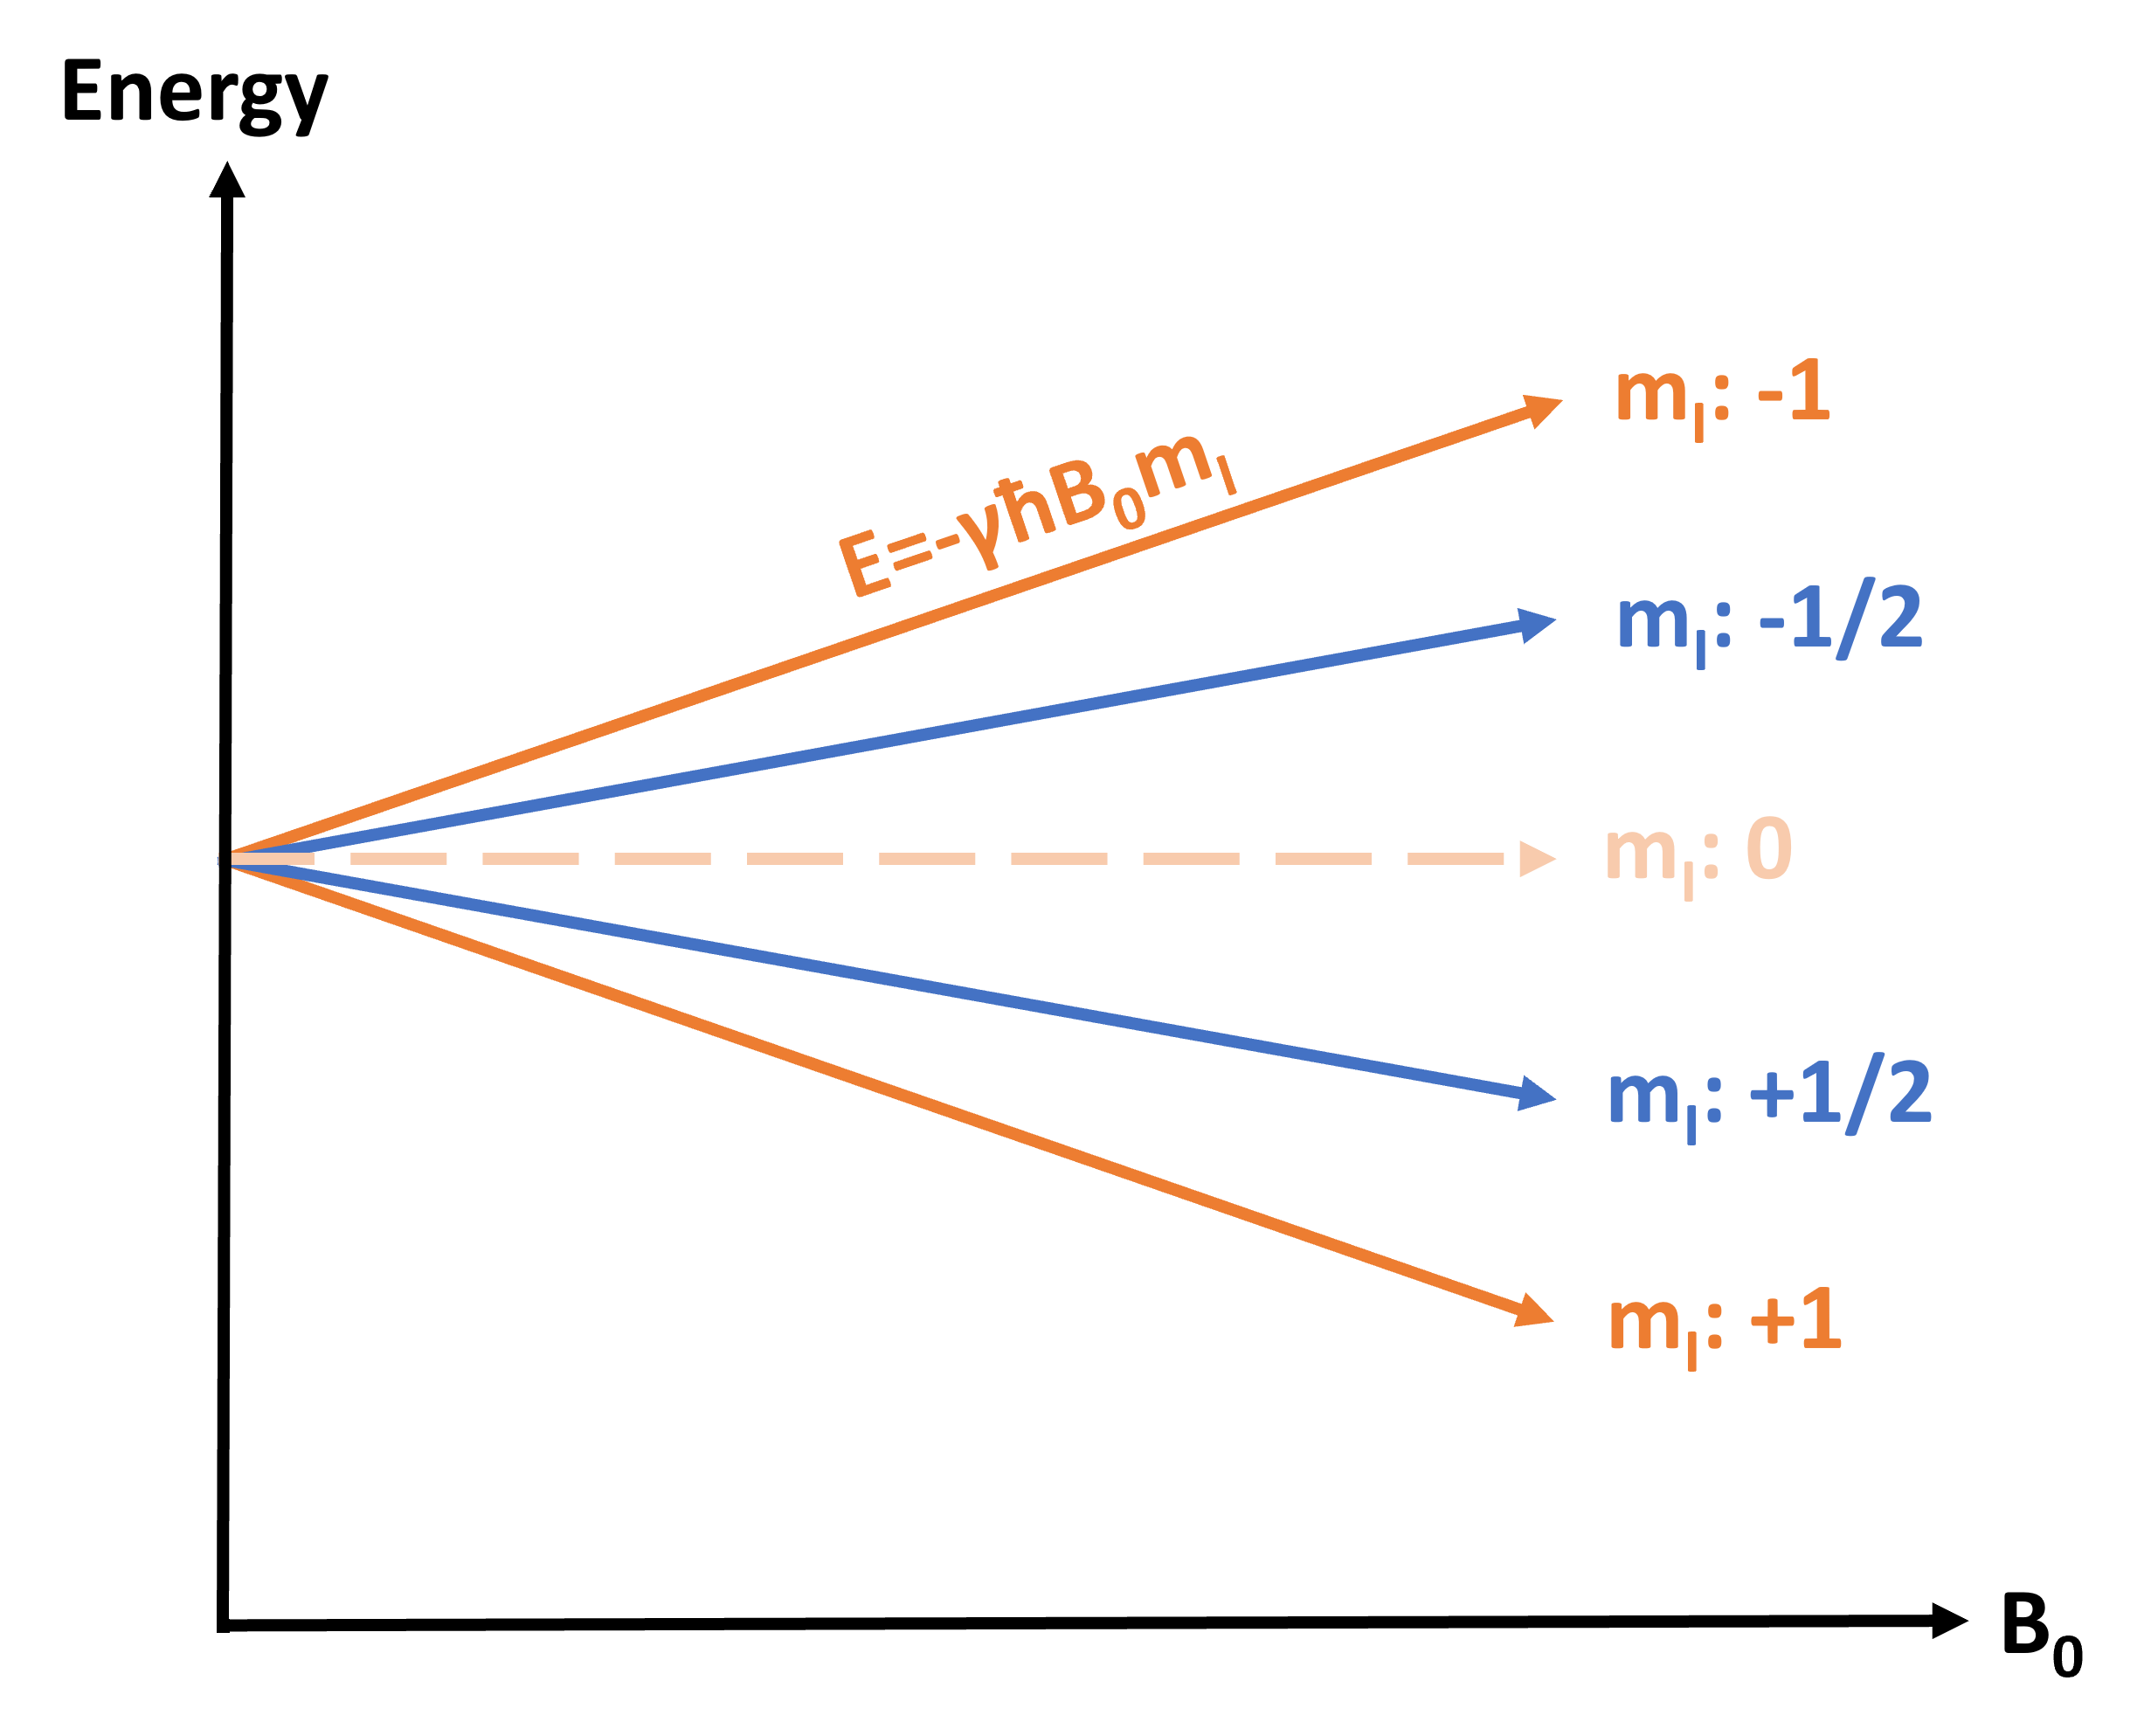
\includegraphics[width=0.8\textwidth]{Figures/Theory/Zeeman.png}
    \caption{\textit{Figure demonstrating the change in spin energy levels due to increasing magnetic field B$_0$, for spin-1/2 and spin-1 nuclei. Demonstrating the Zeeman Effect \cite{Zeeman1896VerslagenAfdeeling}.}}
    \label{fig:theory:zeeman}
\end{figure}

This gives a good overview of how individual spins act and behave in magnetic fields, however our bodies contain a collection of spins of different nuclei. Therefore, it is important to apply these relationships to a collection of spins which will give an overview of macroscopic behaviours that make up the theory of \ac{NMR}.

\subsection{Macroscopic Behaviour}

The molecules of interest for \ac{MRI} are in the liquid state which means the motion of the spin is largely random and due to Brownian motion, thermal energy then becomes the dominant driving force and therefore quantum effects become negligible. When particles have a large enough temperature ($T$) and there are enough particles, the distribution over multiple energy levels can be described according to the Boltzmann distribution \cite{Boltzmann1872WeitereGasmolekulen}. Equation \ref{eqn:theory:boltz} states the probability $p_i$ of a single particle being in a specific state.

\begin{equation}
    p_i = \frac{\exp\left(\frac{-E_i}{k_BT}\right)}{\displaystyle \sum_{j = 1}^{M}\exp\left(\frac{-E_j}{k_BT}\right)}
    \label{eqn:theory:boltz}
\end{equation}

\noindent where $i$ indicates the specific energy level and $M$ is the total number of available states for a specific nucleus. The overall magnetic field that results from a large group of spins can be described by a vector called the magnetisation ($M$). Most of the spins' contributions will cancel so the contribution to the magnetisation vector arises from the difference in the populations of the different energy levels. A generalised summation that yields the equilibrium magnetisation is shown in Eq. \ref{eqn:theory:mag}.

\begin{equation}
    M = N\sum_{j = 1}^{M}p_j\mu_j
    \label{eqn:theory:mag}
\end{equation}

\noindent where $N$ is the number of spins of interest. 

A major assumption that can be made, is that the thermal energy at room temperature is much larger than the nuclear magnetic energies ($\gamma \hbar B_0\ll k_BT$). This gives the simplified version of Eq. \ref{eqn:theory:mag} that is still general to all spins shown in Eq. \ref{eqn:theory:mag_s},

\begin{equation}
    M = \frac{s(s+1)\gamma^2 \hbar^2 N B_0}{3k_BT}
    \label{eqn:theory:mag_s}
\end{equation}

\noindent most nuclei that are of interest for \ac{NMR} have a spin-1/2, which give two distinct energy levels. Equation \ref{eqn:theory:mag_1H} calculates the equilibrium magnetisation for spin-1/2 nuclei, Eq. \ref{eqn:theory:mag_2H} calculates the equilibrium magnetisation for spin-1 nuclei such as $^2$H.

\begin{equation}
    M_0 = \frac{\gamma^2 \hbar^2 N B_0}{4k_BT}
    \label{eqn:theory:mag_1H}
\end{equation}

The equilibrium magnetisation is responsible for the signal produced in \ac{NMR} experiments. It is proportional to the total number of spins and inversely proportional to temperature (measured in kelvin). The temperature will mostly remain constant for experiments performed in humans \textit{in vivo}. Also, $M$ is proportional to the magnitude of any applied external magnetic field applied ($B_0$). The presence of equilibrium magnetisation alone is not enough for \ac{NMR}/\ac{MRI} to produce vital \textit{in vivo} information about the human body. It is also important to be able to manipulate the magnetisation \cite{Haacke2014MagneticDesign}. 

\subsection{Manipulating Magnetisation}

\begin{figure}
    \centering
    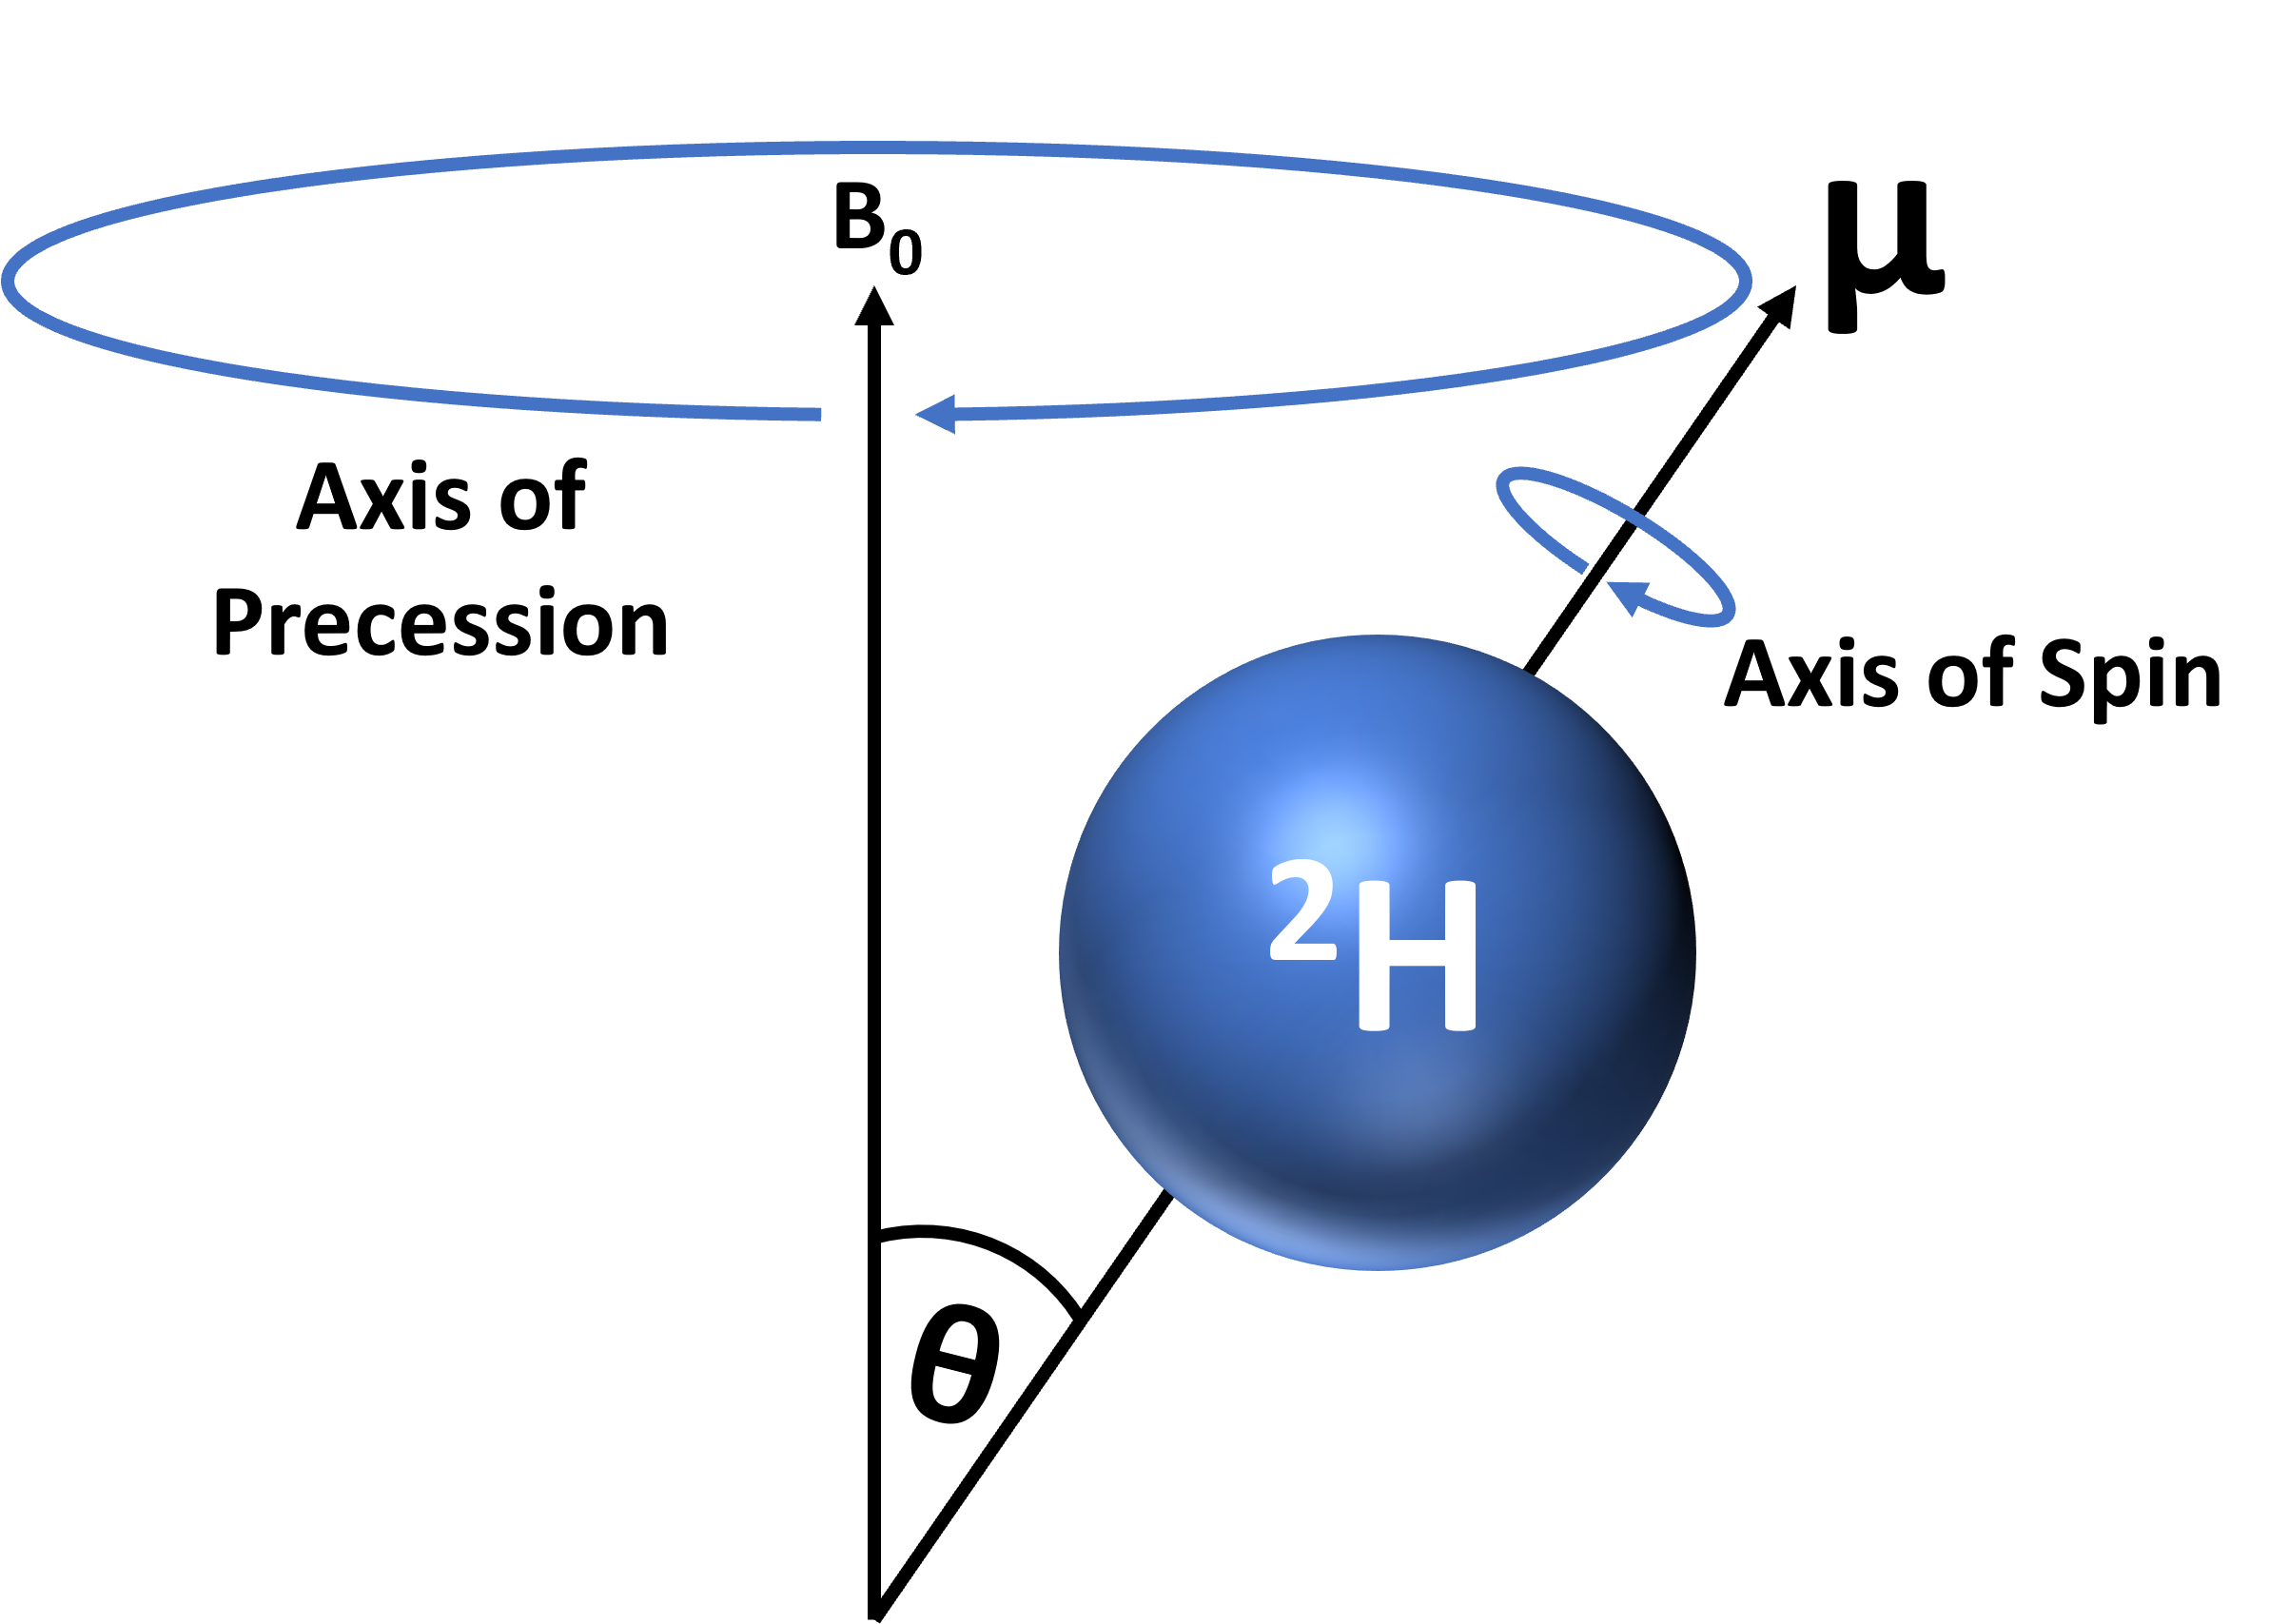
\includegraphics[width=0.9\textwidth]{Figures/Theory/Moment.png}
    \caption{\textit{A diagram of a $^2$H nucleus spinning and precessing around an applied external magnetic field B$_0$. Its magnetic moment $\mu$ and both axes are labelled, along with the angle the magnetic moment vector makes to B$_0$.}}
    \label{fig:theory:moment}
\end{figure}

The direction of the equilibrium magnetisation vector is the same as the applied field. In general magnetisation is made up of two main components, the longitudinal and the transverse. The longitudinal component is parallel to the applied field, with the transverse component being a combination of the two other orthogonal directions. Often the applied magnetic field, and analogously the magnetisation, is defined as $\mathbf{B}=B_0\mathbf{z}$ and therefore the longitudinal component is in the z-direction, which makes the transverse component a combination of the x and y components. The transverse magnetisation (M$_{xy}$) is zero at equilibrium. After a large enough period of time in an applied field the longitudinal magnetisation will reach the value outlined in Eq. \ref{eqn:theory:mag_1H} (M$_0$), whilst the transverse component will remain at zero. The evolution of the longitudinal and transverse components of the magnetisation is described by the Bloch Eq. \cite{Bloch1946NuclearInduction}.

\begin{equation}
    \frac{d\mathbf{M}}{dt} = \, \gamma\mathbf{M}\textrm{x}\mathbf{B} \, + \, \frac{M_0-M_z}{T_1}\mathbf{z} \, - \, \frac{\mathbf{M_{xy}}}{T_2}
    \label{eqn:theory:Bloch}
\end{equation}

The first term in Eq. \ref{eqn:theory:Bloch} describes the evolution of the magnetisation in the presence of a magnetic field $\mathbf{B}$. The second term describes the evolution of the longitudinal magnetisation due to longitudinal relaxation, where T$_1$ is the longitudinal or spin-lattice relaxation time constant. This relaxation, results from spins interactions with the surrounding `lattice'. The final term describes how the transverse magnetisation evolves over time, where T$_2$ is the transverse or spin-spin relaxation time constant. It arises from dephasing due to each spin's interaction with neighbouring spins. 

The transverse relaxation time described here relates to the case where the applied field is perfectly homogenous. However in reality this is rarely the case. In the presence of field inhomogeneity spins dephase more rapidly and the relevant relaxation is T$_2^*$.

\begin{equation}
    \frac{1}{T_2^*} = \frac{1}{T_2} + \frac{1}{T_2^{'}}
    \label{eqn:theory:trans}
\end{equation}

Here T$_2^{'}$ is dependent only on the homogeneity of the field. This means that T$_2^*$ can change between scans and scanners. The relaxation times T$_1$ and T$_2^*$ are specific for each nuclei, tissue type and field strength. In spectroscopy the \ac{FWHM} of each peak, which is a measure of the broadness of peak, is related to the total transverse relaxation (\ac{FWHM}$ = 1 / \pi T_2^*$). 

%The Bloch equation can then be separated for each component ($x,y,z$) and made specific for each experiment, for example there is the static field case substituting $\mathbf{B}=B_0\mathbf{z}$, or it is possible to flip the magnetisation into the transverse plane using $\mathbf{B}=B_0\mathbf{z}+B_1\mathbf{x}$. 

\begin{figure}
    \centering
    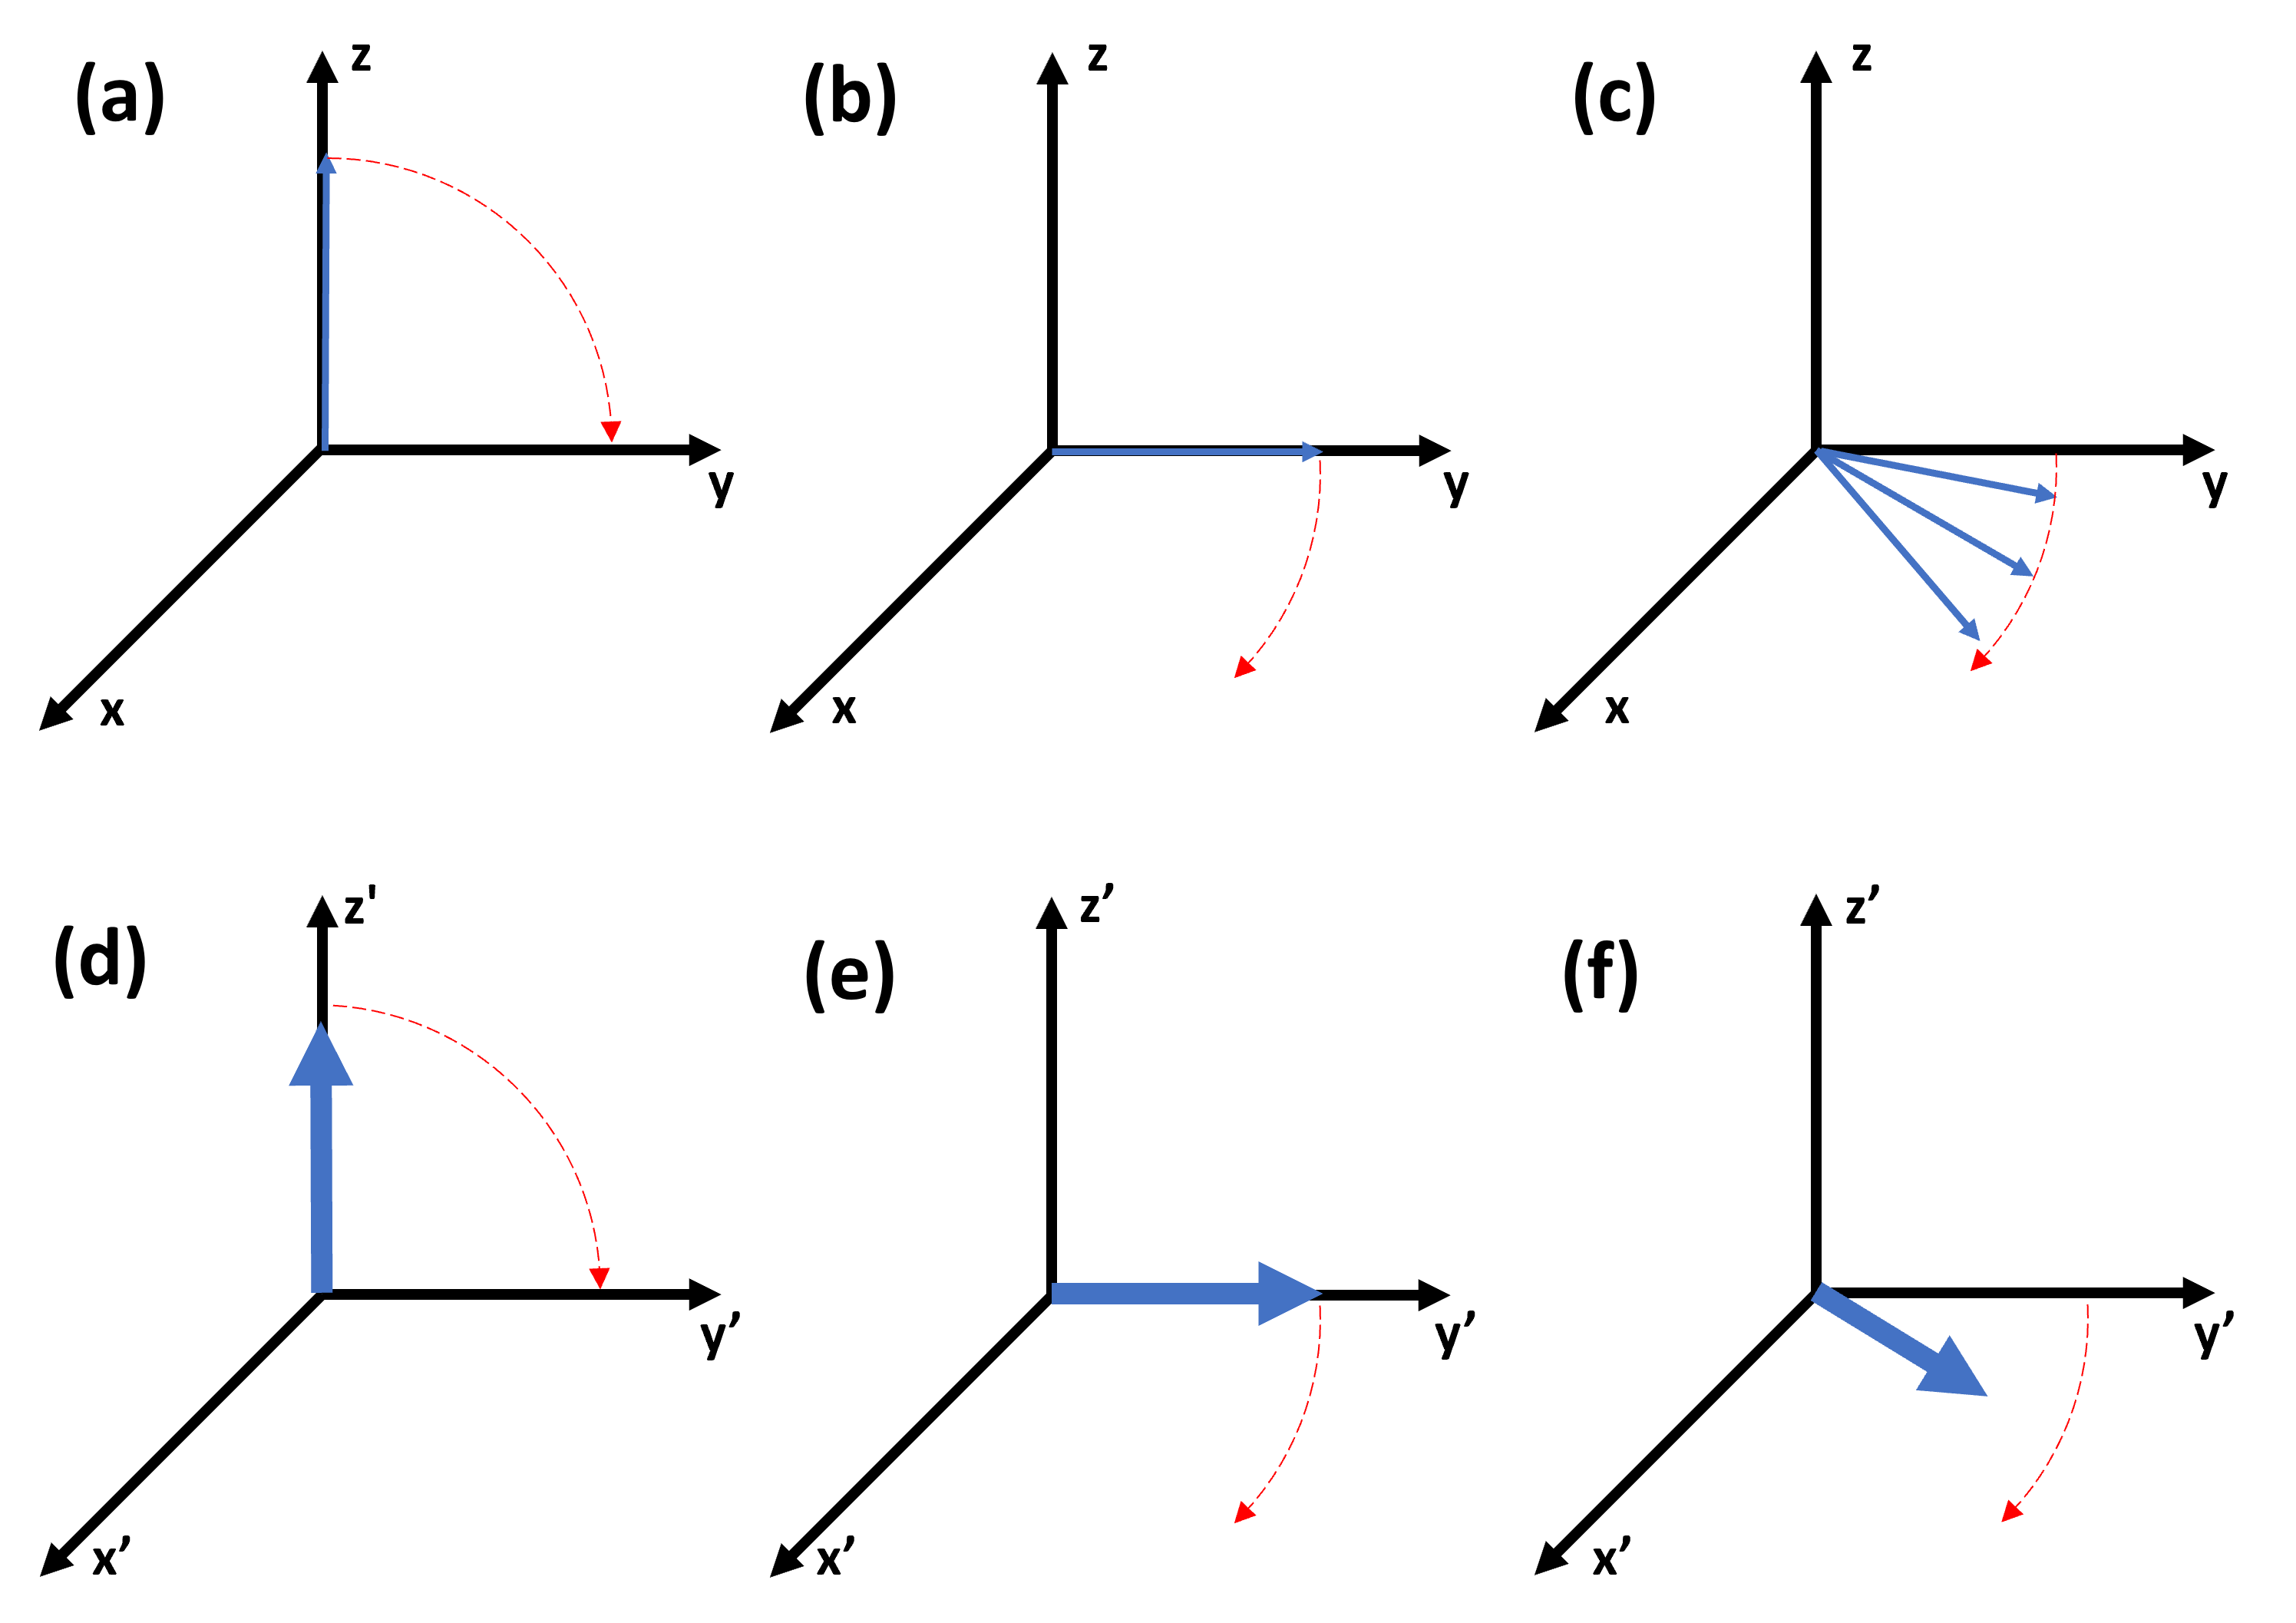
\includegraphics[width=0.9\textwidth]{Figures/Theory/Magnetisation.png}
    \caption{\textit{Diagram showing the effect of applied external magnetic fields on magnetic moment vectors and magnetisation.(a) Shows the precession of a collection of magnetic moment vectors after a static magnetic field (B$_0$) is applied in the z-direction, and just before a 90$^\circ$ degree pulse (B$_1$) is applied. (b) Here the magnetic moments have been tipped to all align in the positive y-direction by an applied 90$^\circ$ \ac{RF} with $B_1$ along $x$ in the rotating frame. (c) After the \ac{RF} pulse the spins begin to dephase due to field inhomogeneity, with the spins `fanning' out in the x-y plane until no overall transverse magnetisation is left. (d-f) Show the spins experiencing the same B$_0$ and B$_1$ as in (a-c) except now only the overall magnetisation vector is shown in the rotating reference frame.}}
    \label{fig:theory:Mag}
\end{figure}


The \ac{NMR} signal arises from the longitudinal magnetisation, however this is very small and can be dominated by magnetisation from electron currents within atoms and molecules. Therefore the magnetisation is usually measured by tipping it into the transverse plane where it undergoes precession and will therefore induce a voltage, at the Larmor frequency in a receiver coil. This tipping is achieved by applying a short alternating magnetic field $\mathbf{B} = B_1\hat{x}\cos (\omega t)$, this is often referred to as an \ac{RF} pulse since the frequency is in the \ac{RF} range.

The precession of magnetisation can be difficult to conceptualise/visualise in a stationary reference frame due to the complex 3D motion. Therefore it is beneficial to consider the system in a rotating frame of reference (ie. as if the observer rotates around the z-axis). The common reference frame used is one that rotates at the frequency of the applied \ac{RF} around the z-axis, this is because the magnetic field of the \ac{RF} pulse is made up of 2 counter-rotating components, one of which will appear as stationary in the rotating reference frame. This gives the following separated Bloch equations for the evolution of magnetization ($x',y',z$) in the rotating reference frame, for a left-circularly polarised \ac{RF} field B$_1$ which is assumed to be parallel to $x'$ in the rotating frame.

\begin{equation}
    \frac{dM_{x'}}{dt} = \Delta\omega M_y^{'} - \frac{M_x^{'}}{T_2}
    \label{eqn:theory:Blochx}
\end{equation}
\begin{equation}
    \frac{dM_{y'}}{dt} = \Delta\omega M_x^{'} + \omega_1M_z^{'} - \frac{M_y^{'}}{T_2}
    \label{eqn:theory:Blochy}
\end{equation}
\begin{equation}
    \frac{dM_z}{dt} = -\omega_1M_y^{'} + \frac{M_0-M_z^{'}}{T_1}
    \label{eqn:theory:Blochz}
\end{equation}

Here, $\omega_1=\gamma B_1$ and $\Delta\omega$ is the difference between the Larmor frequency ($\omega_0$) and the frequency of the rotating reference frame ($\omega$), and represents any off resonance effects. Therefore, if the \ac{RF} is applied at the Larmor frequency, $\Delta\omega=0$ and these terms disappear. If only the static field case is being considered, the $\omega_1$ terms disappear as well, which leaves only the relaxation dominant terms. If short \ac{RF} pulses are considered the solutions to Eqs. \ref{eqn:theory:Blochx} - \ref{eqn:theory:Blochz} describing the evolution of magnetisation after the pulse are shown in Eqs. \ref{eqn:theory:xprime} - \ref{eqn:theory:zprime}.

\begin{equation}
    M_{x'}(t) = \exp(-t/T_2) \left( M_{x'}(0)\cos\Delta\omega t \, + \, M_{y'}(0)\sin\Delta\omega t \right)
    \label{eqn:theory:xprime}
\end{equation}
\begin{equation}
    M_{y'}(t) = \exp(-t/T_2) \left( M_{y'}(0)\cos\Delta\omega t \, - \, M_{x'}(0)\sin\Delta\omega t \right)
\end{equation}
\begin{equation}
    M_z(t) = M_z(0)\exp(-t/T_1) \, + \, M_0 \left( 1-\exp(-t/T_1) \right)
    \label{eqn:theory:zprime}
\end{equation}

RF pulses are used to rotate the longitudinal magnetisation into the transverse plane. In between short applied fields (\ac{RF} pulses) it is often necessary to wait a large enough period of time for the magnetisation to relax back into its longitudinal state before repeating the process to acquire more data. 

% Therefore, whilst the longitudinal magnetisation is important for overall signal it is important to accurately and reliably tip the magnetisation exactly at 90$^\circ$, as deviations in this `flip-angle' ($\theta$) could reduce the available signal \cite{deGraaf2019InSpectroscopy}.

\subsection{Flip Angles, Phase and Signal}

The flip angle ($\theta$) generated from a short \ac{RF} pulse (excitation) is dependent on the B$_1$ magnetic field strength and the pulse duration ($\tau$) according \ref{eqn:theory:FA}.

\begin{equation}
    \Delta\theta = \gamma B_1 \tau
    \label{eqn:theory:FA}
\end{equation}

Where $\theta$ is the angle the magnetisation is rotated through after excitation, also known as the flip-angle. If starting from the equilibrium situation, the closer this flip-angle is to 90$^\circ$ the larger the amount of longitudinal magnetisation that is rotated into the transverse plane. The signal produced by precessing transverse magnetisation can be described as a complex signal such that $f(t) = R(t) + I(t)$. This is known as a \ac{FID}. The signal induced in the receiver coil after a 90$^\circ$ pulse is applied to equilibrium magnetisation can be written as.

\begin{equation}
    R(t) \propto M_0\cos(\omega_0 t+ \phi)\exp(-t/T_2^*)
    \label{eqn:theory:real}
\end{equation}
\begin{equation}
    I(t) \propto -M_0\sin(\omega_0 t+ \phi)\exp(-t/T_2^*)
    \label{eqn:theory:imag}
\end{equation}

\noindent where $\phi$ is the phase of the signal and represents the angle the transverse magnetisation makes to the $x'$ axis after excitation, i.e a phase of -90$^\circ$ would be aligned parallel to the y-axis. $M_0, \, \omega, \, \phi \, \textrm{and} \, 1/T_2^*$ are parameters that were mentioned in the previous section (amplitude, frequency, phase and relaxation rate) respectively. The real and imaginary components can be combined using Euler's formula to give Eq. \ref{eqn:theory:euler}. 

\begin{equation}
    f(t) \propto M_0\exp(-\omega_0 t)\exp(-t/T_2^*)\exp(i\phi)
    \label{eqn:theory:euler}
\end{equation}

This signal is described in the time-domain. To separate different frequency contributions to the signal, it is useful to transform this signal into the frequency domain, which can be performed using a \ac{FT} \cite{Fourier1822TheorieChaleur}. The equation used for doing this is

\begin{figure}
    \centering
    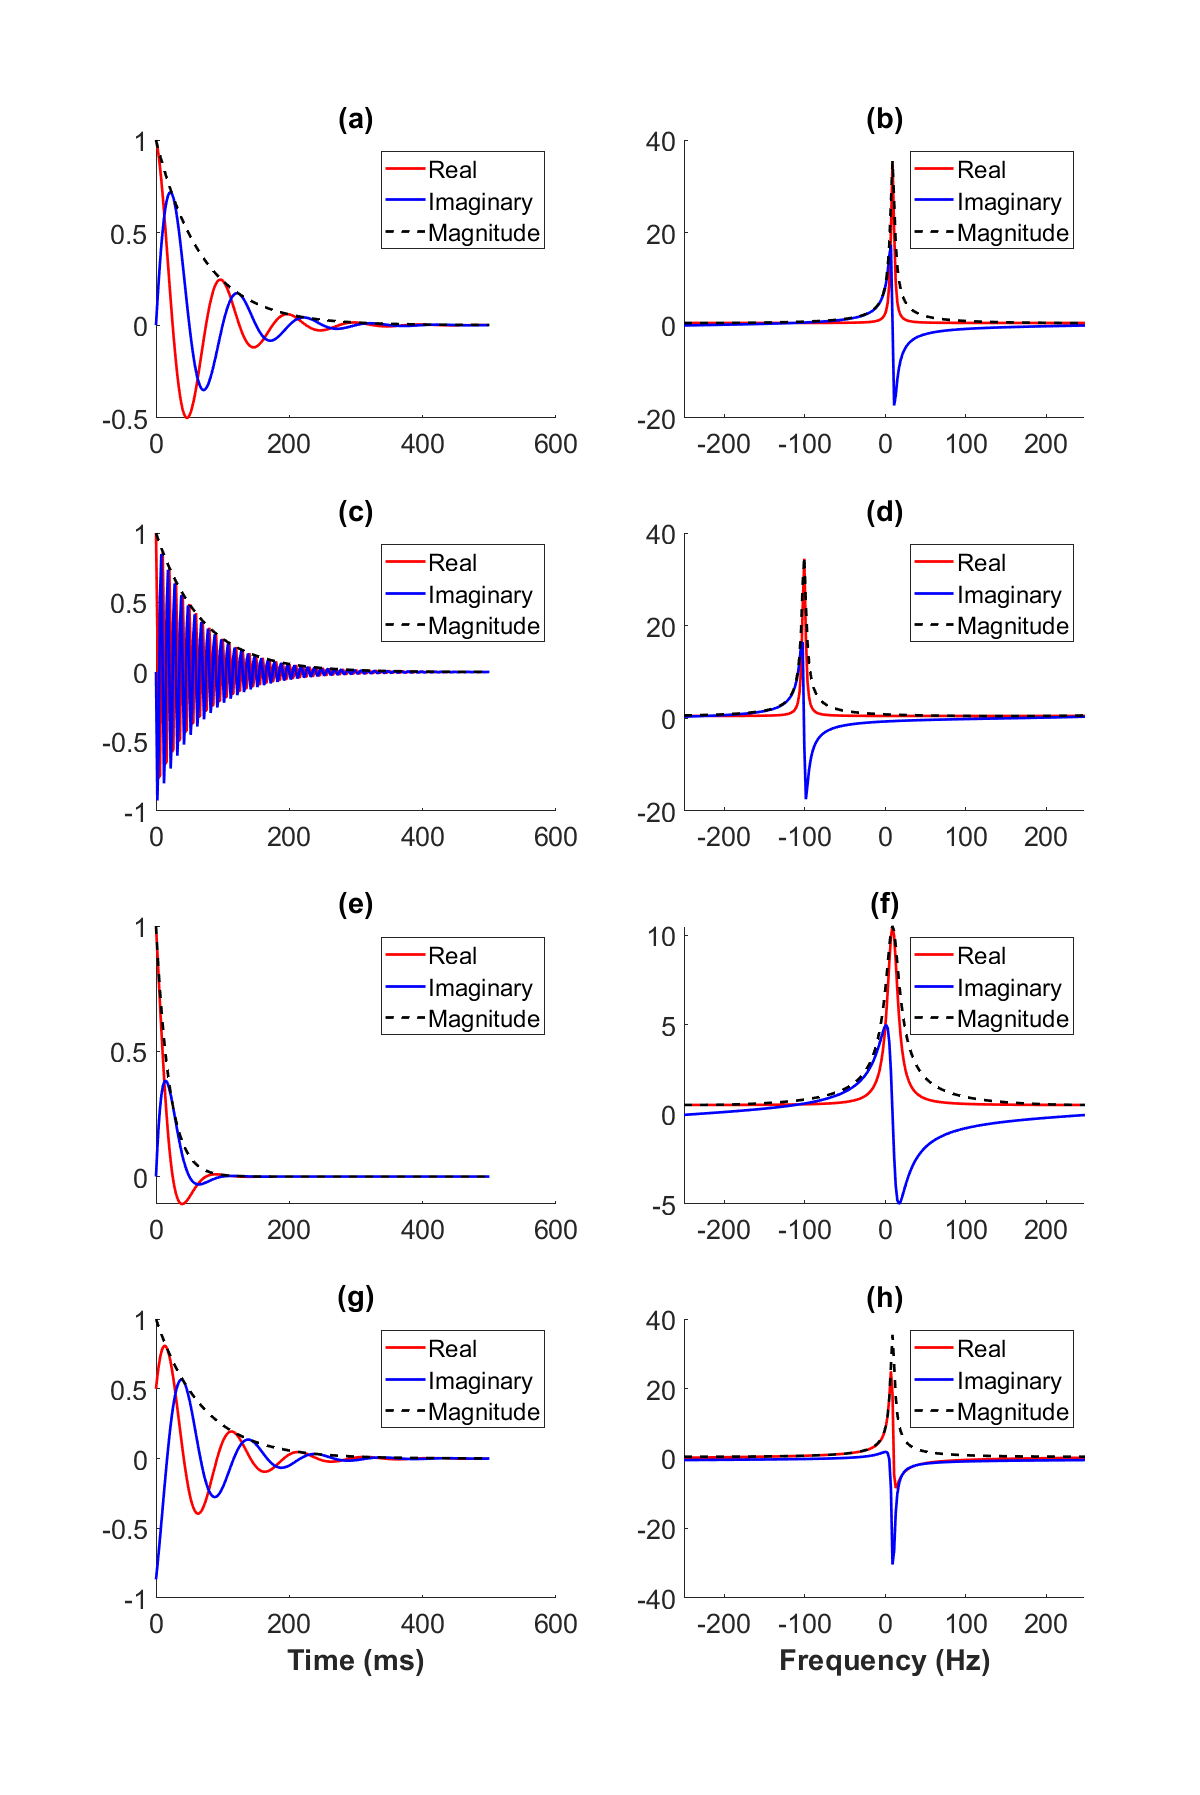
\includegraphics[width=0.9\textwidth]{Figures/Theory/FID_Lorentz.png}
    \caption{\textit{Plots of \ac{FID}s (left) and corresponding lineshapes (right) for different frequency offsets ($\nu_0$), transverse relaxation times (T$_2^*$) and phases ($\phi$), all FIDs have an amplitude ($A$) of 1. The parameters for (a) and (b) are $\nu_0$=-10 Hz, T$_2^*$= 70 ms and $\phi$=0, one parameter is changed in each row. (c) and (d) have a different $\nu_0$ of +100 Hz. (e) and (f) have a shorter T$_2^*$ of 20 ms. (g) and (h) have a phase of $\phi$=-$\pi$/3.}}
    \label{fig:theory:FID_Lorentz}
\end{figure}

\begin{equation}
    F(\omega) = \int_{-\infty}^{+\infty} f(t)\exp(-\omega t) \, dt
    \label{eqn:theory:fourier}
\end{equation}

\noindent where $F(\omega)$ is the frequency domain spectrum, $\omega$ is the angular frequency. By applying a \ac{FT} to the \ac{FID} where signal is only present  for $t > 0$ Eq. \ref{eqn:theory:lorentz} is obtained (with $\nu = \omega/2\pi$), which depends on the same four parameters as the \ac{FID}. The relationship between the T$_2^*$ and the FWHM has already been described: as the T$_2^*$ gets longer, the peak becomes narrower. It is important to note however that the integral/area under the peak is independent of T$_2^*$. The integral only depends on the amplitude (A) of the signal. Therefore, the shorter the T$_2^*$ the smaller the peak height and \textit{vice versa}, and therefore maximising A and T$_2^*$ maximises the available \ac{SNR} in the spectrum. With $R_2^* = 1/T_2^*$

\begin{equation}
    F(\nu) = A\exp(i\phi)\frac{R_2^*-i2\pi(\nu-\nu_0)}{R_2^{*2}+4\pi^2(\nu-\nu_0)^2}
    \label{eqn:theory:lorentz}
\end{equation}

Using \ac{NMR} to measure signals from pure samples with only one nuclear magnetic resonance will produce spectra with single peaks. However in general samples contain a range of different molecules, in which the atoms of each atomic species can be in different chemical environments. This is certainly the goal for \ac{MRS} measurements on living systems. The shielding of the magnetic field at the nucleus by the surrounding electron cloud changes the magnetic field at the nucleus, which in turn changes the resonant frequency of precession for nuclei. Therefore, nuclei that have different chemical environments will precess at different frequencies which means that the \ac{NMR} signal will be found at different frequency positions in an \ac{NMR} spectrum. Therefore by identifying the positions of peaks in an \ac{NMR} spectra and finding the amplitudes of the peaks, it is possible to probe the chemical structure of the compounds found in the sample. This is useful in studies of medical conditions and diseases. The main unit of measure for frequency is hertz (Hz), however the values here will change greatly depending on the nuclei of interest and the field strength being used. Therefore a different unit of measurement is often used to characterise the frequency in \ac{NMR} spectra to make it more general and therefore applicable to all nuclei and field strengths. The chemical shift ($\delta$) of each signal is measured in parts-per-million (ppm). The equation to calculate chemical shift from frequency is shown in Eq. \ref{eqn:theory:chemshift}.

\begin{equation}
    \delta = \frac{\nu - \nu_{\textrm{ref}}}{\nu_\textrm{ref}} \, \textrm{x} \, 10^6
    \label{eqn:theory:chemshift}
\end{equation}

Where $\nu_{\textrm{ref}}$ is a reference frequency. So far it has been outlined how to obtain an \ac{NMR} signal in samples and in the body using MRS. However, sometimes it is not enough to just obtain information on the chemical structures/composition of the body and spatial information is also needed to interrogate chemical compositions of specific areas in the body. The most common way to do the required spatial encoding is to use magnetic fields that vary spatially \cite{Haacke2014MagneticDesign}. 

\subsection{Introduction of Gradients}

According to Eq. \ref{eqn:theory:Lamor} the frequency of precession is dependent on the applied magnetic field. Therefore if the magnetic field varies with spatial position the frequency of precession will also vary with spatial position. In particular a magnetic field gradient corresponding to the linear variation of field with position, produces a linear variation of frequency with position. For example when a gradient is applied in the $z$-direction.

\begin{equation}
    B_z = Gz,\; \omega = \gamma Gz 
\end{equation}

Previously, we considered the situation where a static spatially-homogeneous $B_0$ was applied to a sample and an \ac{RF} pulse was used to tip the magnetisation of all the spins into the transverse plane. However if a gradient is applied along with B$_0$, only the spins with the same frequency as the \ac{RF} pulse will be tipped. The magnetic field in the presence of a gradient is described by Eq. \ref{eqn:theory:B_Grad}, with the frequency that is spatially dependent is shown in Eq. \ref{eqn:theory:f_Grad}.

\begin{equation}
    B(r) = B_0 \, + \, Gr
    \label{eqn:theory:B_Grad}
\end{equation}

\begin{equation}
    \nu(r) = \frac{\gamma}{2\pi}(B_0 \, + \, Gr)
    \label{eqn:theory:f_Grad}
\end{equation}

\noindent Here $r$ is used to represent any cartesian spatial co-ordinate. Therefore only a spatially localised `slice' will be excited and any signal received will be specifically from that slice. By changing the frequency of the applied \ac{RF} pulse different slices can be excited. If the pulse contains a range of frequencies (bandwidth) all the frequencies in the bandwidth will be excited, this results in a slice being excited that has a finite thickness. If this process is repeated, signals can be acquired from multiple slices and therefore the changes in signals can be compared to position in the body of which the slice was acquired. The link between magnetic field/frequency and position using gradients is demonstrated visually in Fig. \ref{fig:theory:Grad}.

\begin{figure}
    \centering
    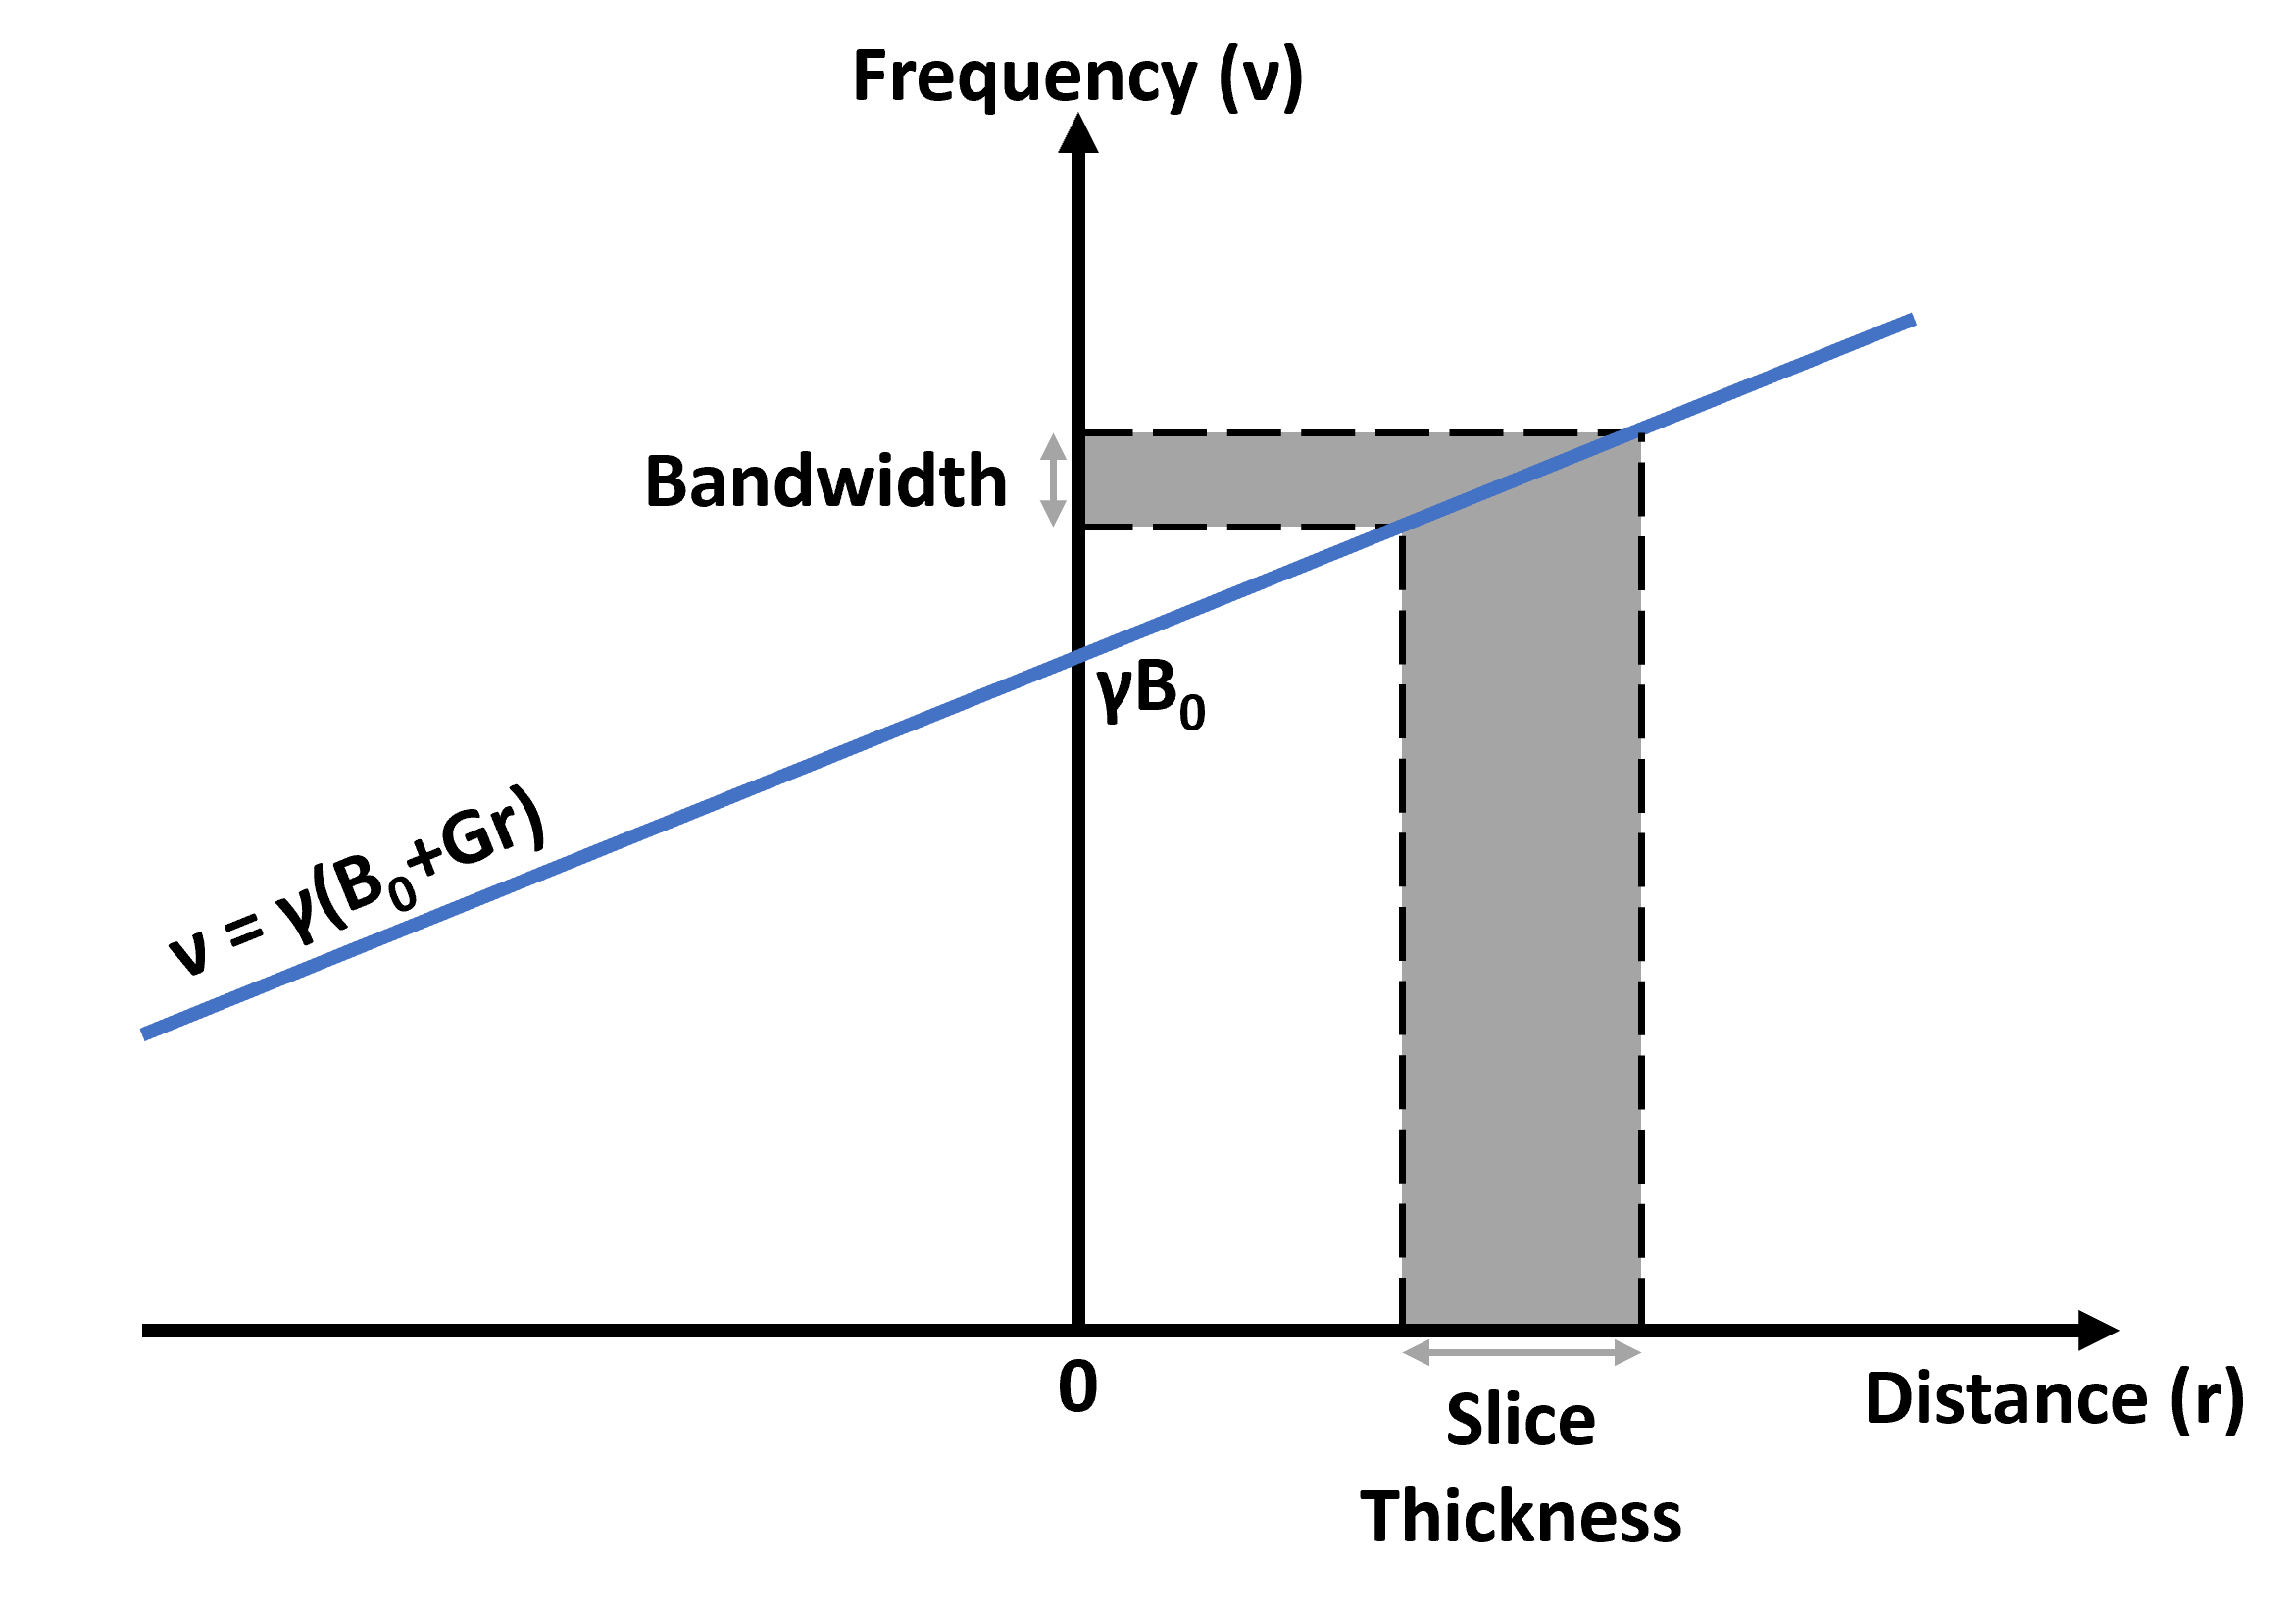
\includegraphics[width=0.9\textwidth]{Figures/Theory/Gradient.png}
    \caption{\textit{The relationship between frequency of precession ($\nu$) and thickness of an acquired slice when a gradient ($G_{slice}$) is applied.}}
    \label{fig:theory:Grad}
\end{figure}

If the chemical composition of what is being investigated is not important it is possible to acquire entirely spatial information and create a volumetric image based on multiple slices. To perform this process gradients are applied in more dimensions than just the slice-selective gradient \cite{deGraaf2019InSpectroscopy}.

\section{Differences for $^2$H}

Deuterium ($^2$H) is a stable isotope of hydrogen. The nucleus of a $^2$H atom is called a deuteron. Large elements are formed in supernovas \cite{Watson2019IdentificationStars}, whilst lighter elements up to iron are made in the cores of stars during fusion. However, $^2$H is destroyed very quickly in fusion within stars \cite{Patrignani2016ReviewPhysics} therefore almost all the $^2$H that exists naturally is formed from Big Bang Nucleosynthesis \cite{Joseph2023GeologicalEarth}. The 0.015\% $^2$H abundance found in the Earth's oceans is similar to what has been found in comets, which adds evidence that ocean water originates from comets \cite{Hersant2001APlanets}. Most of the natural $^2$H content occurs as \ac{HDO}, and the $^2$H content of different water sources (oceans, rainwater etc) can be used to track the water cycle \cite{Bowen2019IsotopesApplications}. Our bodies consequently have a very low natural abundance (NA) $\approx$0.015\% of $^2$H, which makes $^2$H appealing for tracer studies, as small concentration increases are easy to detect above baseline. The addition of a neutron to the nucleus of $^2$H means the gyromagnetic ratio ($\gamma$) is smaller than that of $^1$H (6.54 vs 42.6 MHzT$^{-1}$) which reduces the Larmor frequency of $^2$H according to Eq. \ref{eqn:theory:Lamor}. A magnetic moment is a vector quantity that is used to describe magnetic fields and interactions that arise from charges. Dipolar moments arise from charge distributions and point dipoles, a quadrupolar moment is a second rank expansion of the dipolar moment and is used to describe non-spherical charge distributions. $^2$H has an integer spin of 1 and due to the non-symmetric distribution of charge within the nucleus also has a quadrupolar magnetic moment of 0.286 fm$^2$. The nuclear quadrupolar moment interacts with local electric field gradients, and fluctuations in this interaction cause relaxation, thus reducing both the longitudinal and transverse relaxation times of quadrupolar nuclei. Deuterium's spin of 1 also introduces an extra Zeeman energy level more than for $^1$H, with allowed values of $m_s$ = -1, 0 and 1. Considering that the magnetisation is the net vector sum of $\mathbf{\mu}$ the net magnetisation is due to the population differences 
across energy levels. Using Eq. \ref{eqn:theory:mag} and/or \ref{eqn:theory:mag_s} a simplified equilibrium magnetisation can be found, which is shown in Eq. \ref{eqn:theory:mag_2H}.

\begin{equation}
    M_0 = \frac{2\gamma^2 \hbar^2 N B_0}{3k_BT}
    \label{eqn:theory:mag_2H}
\end{equation}

Whilst the magnetisation appears to be 8/3 larger for $^2$H compared to $^1$H in Eq. \ref{eqn:theory:mag_2H}, it is important to note $M_0$ is also dependent on the gyromagnetic ratio squared along with the number of spins. The gyromagnetic ratio squared is $\approx$42 times smaller for $^2$H. Also assuming the mass and volume of the sample/tissue being scanned/investigated is at \ac{NA} the number of spins will be $\approx$6.7x10$^{-3}$ smaller for $^2$H. The lower value of $\gamma$ also reduces the Larmor frequency, leading to a further reduction in the NMR signal. This reduction in $\gamma$ means stronger gradients are needed to produce the same amount of spatial encoding. Some of the loss in signal of $^2$H can thankfully be recovered due to the reduction in relaxation times. This is because the signal will return to equilibrium more rapidly and therefore the scans can be more rapidly repeated and averaged, increasing the number of averages that can be acquired per unit time. The decrease in \ac{SNR} for $^2$H compared to $^1$H makes \ac{MRI} difficult at \ac{NA}, which is why spectroscopic techniques are much more common for $^2$H. 

% \subsection{Other Nuclei} Potential subsection
% Carbon-13, Phosphorous-31

\section{Scanning}   

\subsection{Imaging}

\begin{figure}[h]
    \centering
    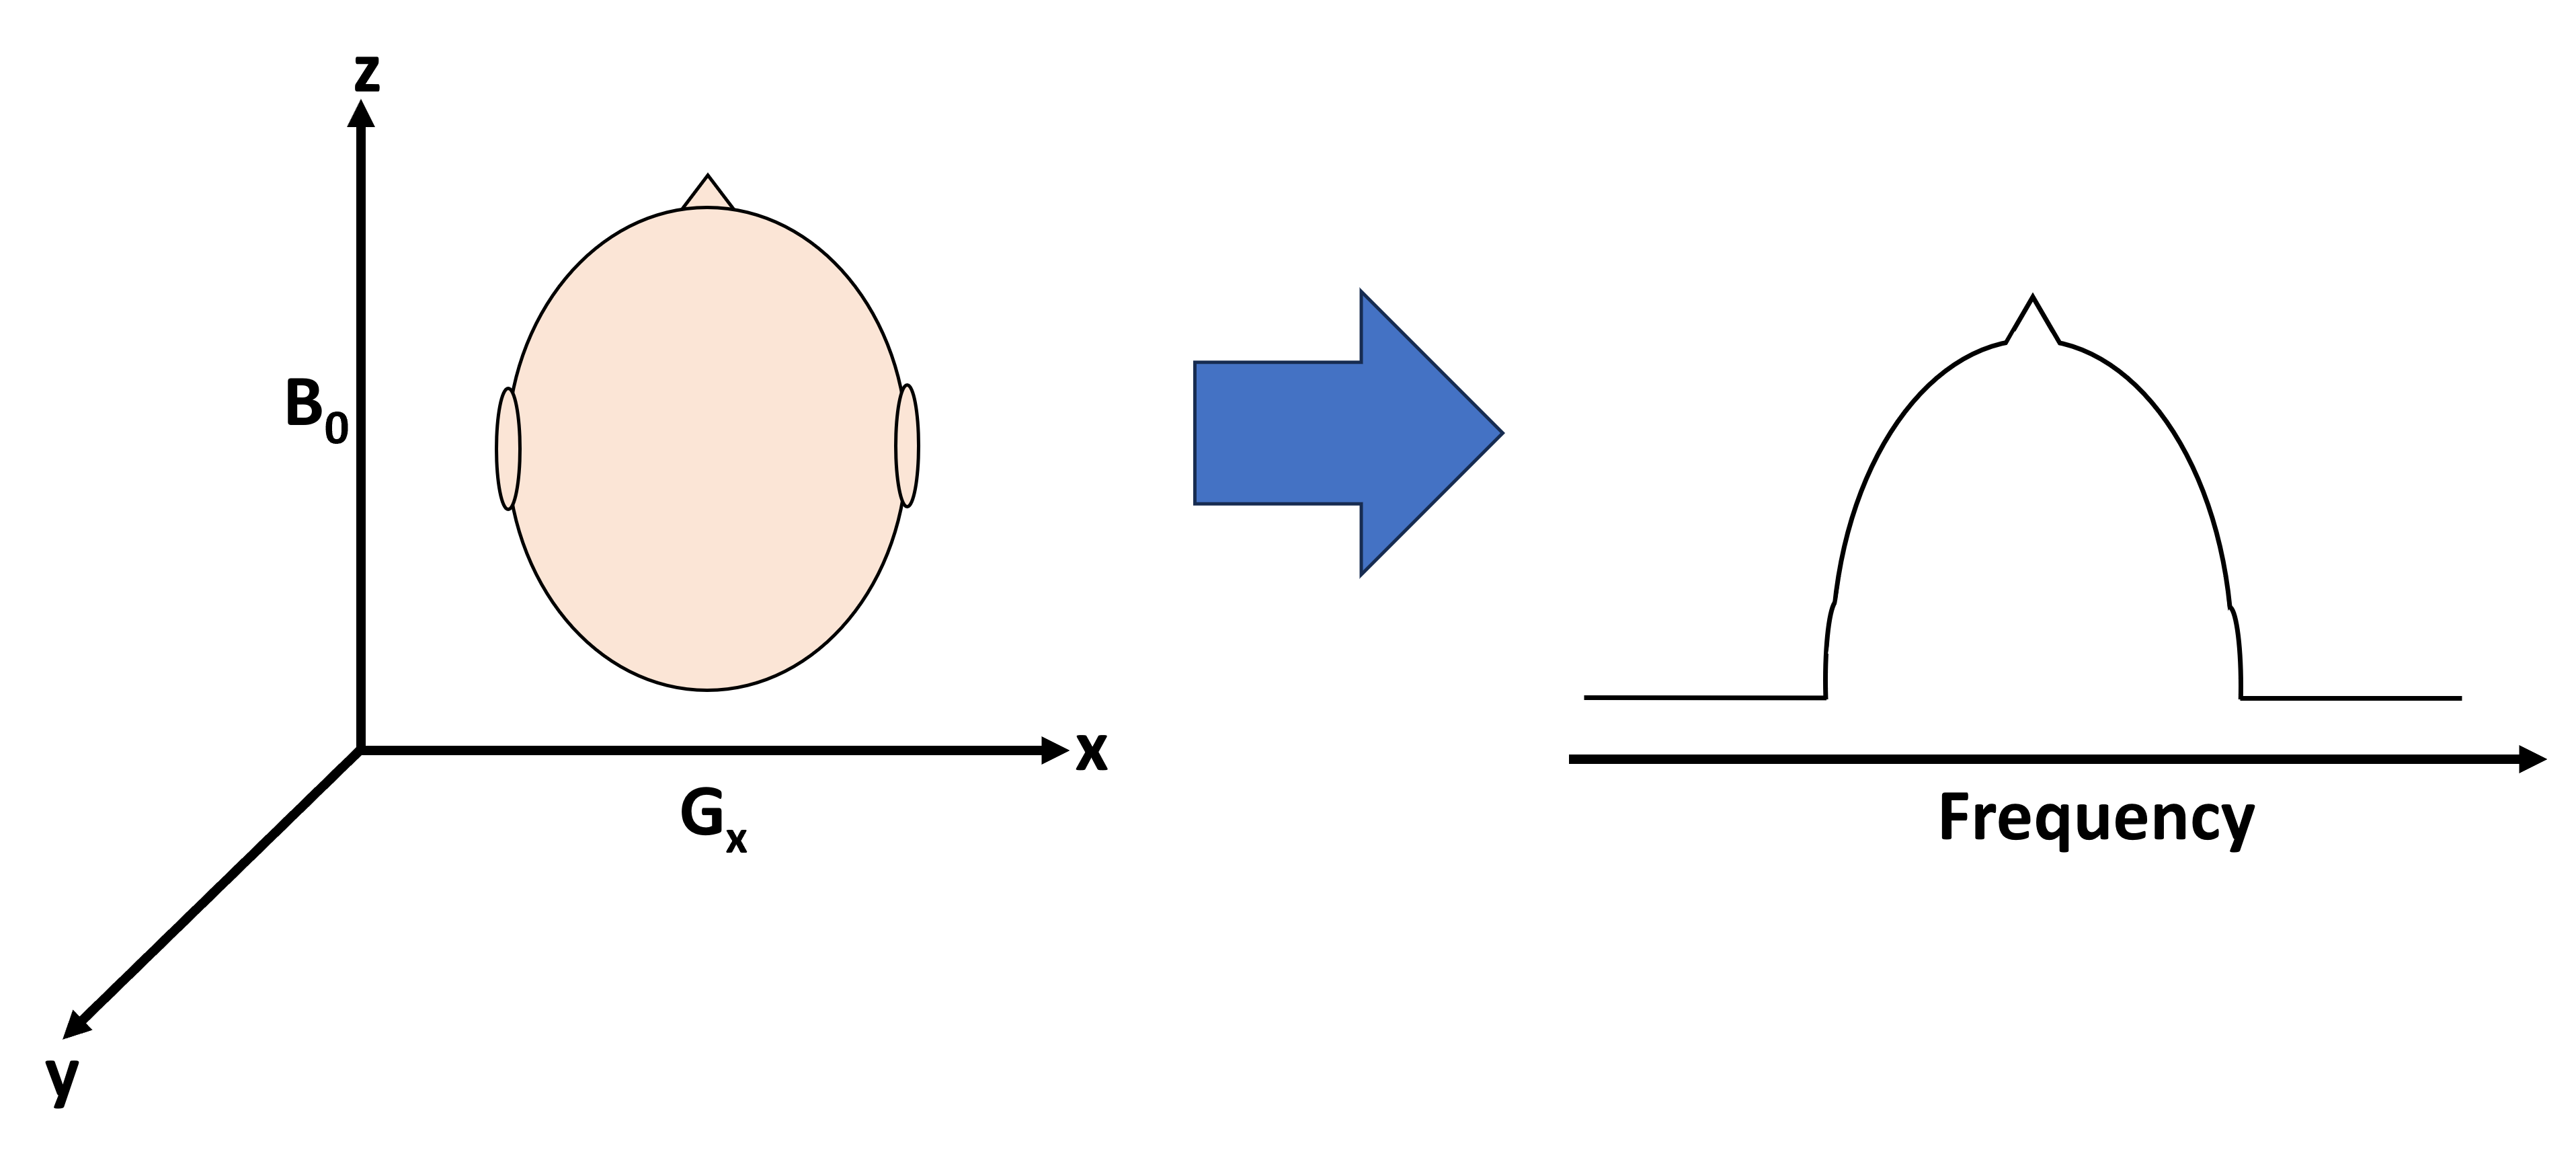
\includegraphics[width=1\textwidth]{Figures/Theory/1D_Projection.png}
    \caption{Diagram showing how a 1D projection of an image is created using a gradient applied in the x direction.}
    \label{fig:theory:1D}
\end{figure}

The use of gradients during \ac{RF} pulse excitation to excite signals selectively within a thin slice of the object, known as slice selection, is the first step in using magnetic fields to obtain images. In addition to slice selection two more directions also need to be encoded. If a gradient is applied immediately after the excitation, the \ac{FID} and corresponding spectrum will contain spatial information, as the frequency shift of peaks will inform on location of the signal in a similar way to the slice selection. The spectrum then represents a 1D projection of the spin density of whatever is being scanned. The spectral width of the obtained signal therefore identifies the width/size of the image which is often linked to the required \ac{FOV} of an image. This method of encoding an additional dimension is known as frequency encoding using a readout/frequency gradient (G$_{\textrm{read}}$/G$_{\textrm{freq}}$), with the obtained 1D spectrum being known as the readout profile.

Whilst frequency encoding does work to obtain an additional dimension, there are real world limitations that can hinder this process. The main limitation is the gradient switching as the turning on/off of the gradient cannot occur instantaneously therefore the first few \ac{FID} points might be acquired during a time-varying gradient which could lead to errors in the data, which will persist into the spectrum after an \ac{FT} is applied. A method of getting around this is to remove first few points from the \ac{FID}, however these contain the highest signal and therefore could reduce the available \ac{SNR}. The realistic method to navigate around this problem is to create an signal at a later time point by taking advantage of dephasing and rephasing, the later signal is referred to as an echo. If the echo is created using a 180$^\circ$ pulse it is referred to as a \ac{SE}, if the echo is created by manipulating gradients it is referred to as a \ac{GE}. When a perfect \ac{FID} is created, the signal starts with a phase of 0 at t=0 and as the magnetisation evolves in the transverse plane it begins to accumulate phase. Therefore by applying a negative G$_{read}$ which encourages the dephasing, followed by a positive G$_{read}$ the phase accumulation reverses in direction during the positive G$_{read}$ and reaches 0 again. Acquiring data at this point allows a full \ac{FID} to be obtained with the maximum signal occurring during the G$_{read}$. The echo occurs at a time referred to as the \ac{TE}. It is important to note that the rephasing only recovers the dephasing caused by the negative G$_{read}$, it does not recover signal lost from T$_2$ or T$_2^*$ relaxation processes. Another type of echo formation exists, called a \ac{SE} or Hahn-echo \cite{Hahn1950SpinEchoes} which involces application of a 180$^\circ$ \ac{RF}pulse after the first set of gradients to rephase the signal, the use of \ac{GE} are often preferred to SE in terms of imaging thanks to the the lower flip angles, shorter \ac{TE} and shorter \ac{TR} that can be achieved. The \ac{TR} is the time from the end of the \ac{RF} pulse until the scan can be repeated. Repeating/averaging the scan allows the \ac{SNR} to be improved.

\begin{figure}
    \centering
    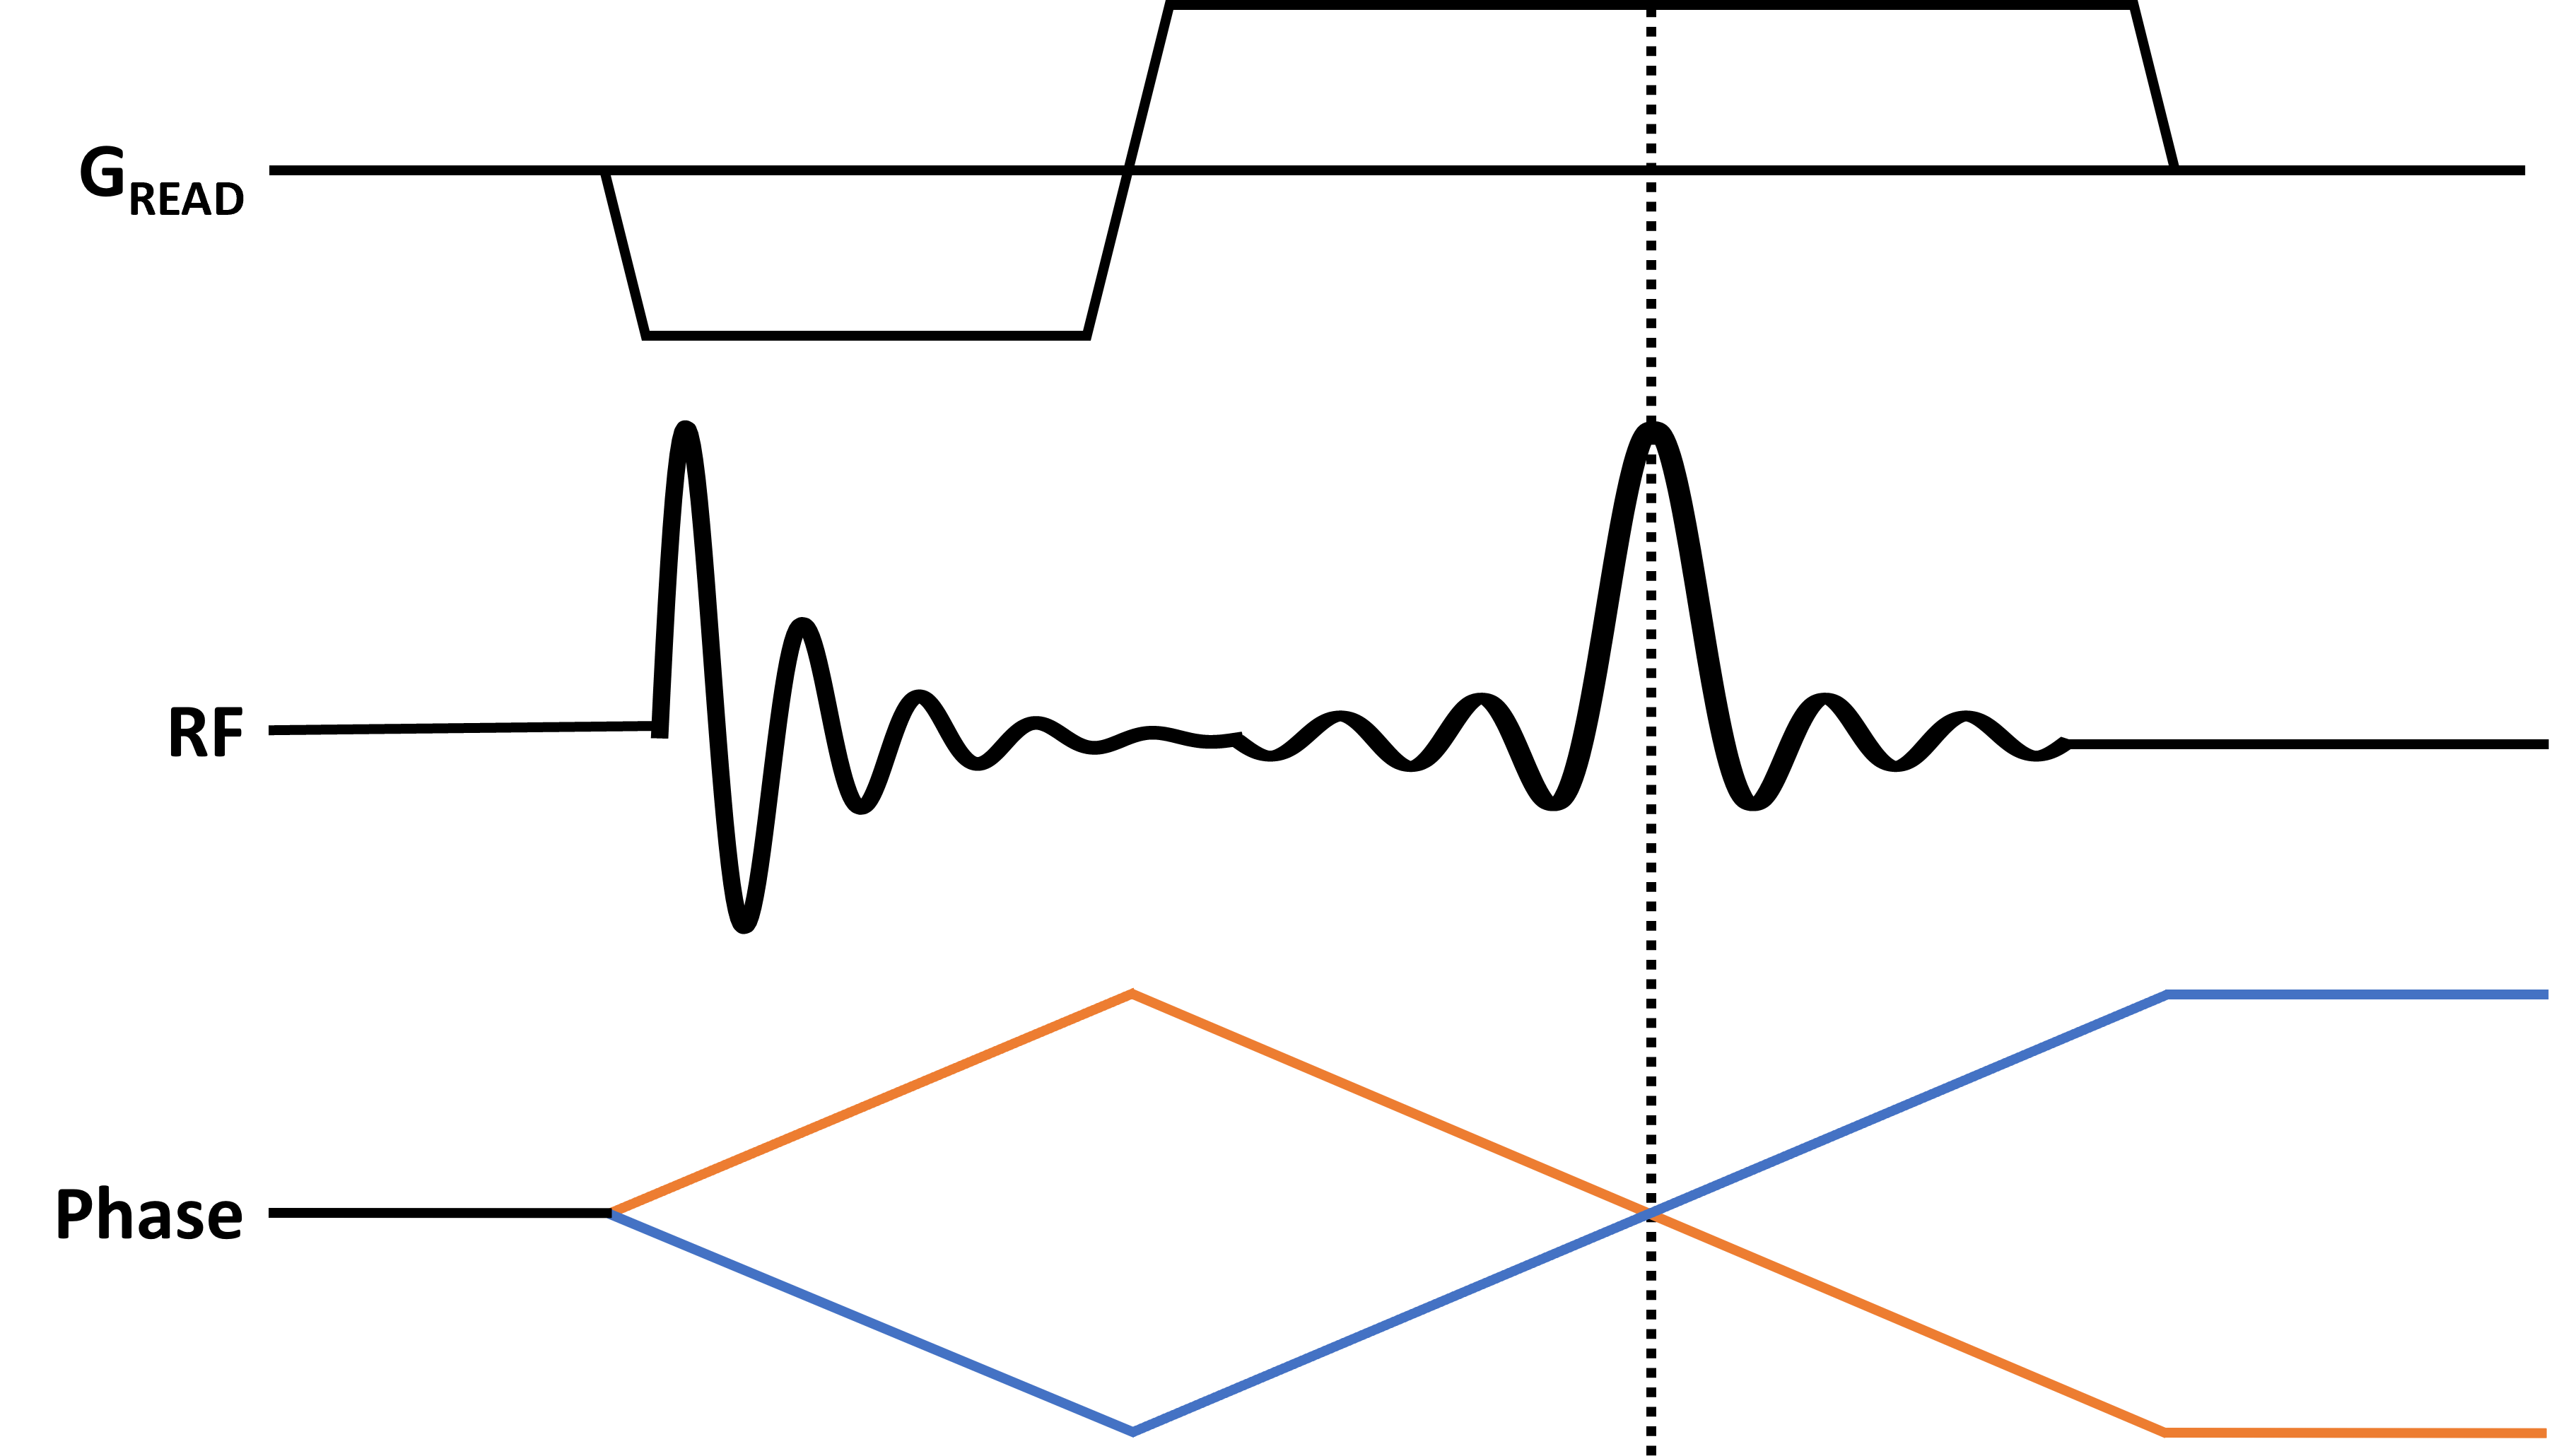
\includegraphics[width=0.9\textwidth]{Figures/Theory/RePhasing.png}
    \caption{Diagram showing how phase accumulation varies with dephasing lobes of the read gradient, along with the received \ac{RF} signal. The blue and orange lines demonstrate the phase changes of two different spins in two different spatial locations. The peak signal during the echo occurs when the phase net phase change for spins is zero, indicated by the dotted line.}
    \label{fig:enter-label}
\end{figure}

The final spatial dimension is often encoded using a phase-encoding gradient (G$_{phase}$) which is applied before the signal is acquired under the read gradient. This gradient only affects the phase of the signal in a way which is dependent on its position in real-space. By linearly changing the magnitude of the applied phase encoding gradient a set of 1D spectra are acquired which can be represented in a 2D matrix. The data in the 2D matrix is therefore a collection of spatial frequencies that are centred on 0. A low spatial frequency describes the general trend of an image whilst the high spatial frequencies define the sharp edges. This frequency space where the data is stored is called k-space, and applying a 2D \ac{FT} to this data produces an image \cite{Lauterbur1973ImageResonance, Mansfield1977Multi-planarEchoes}. The collection of \ac{RF} pulses and gradients is called a pulse sequence, and the pulse sequence described so far is called gradient-echo imaging, and can be viewed in Fig. \ref{fig:theory:GRE}.

\begin{figure}
    \centering
    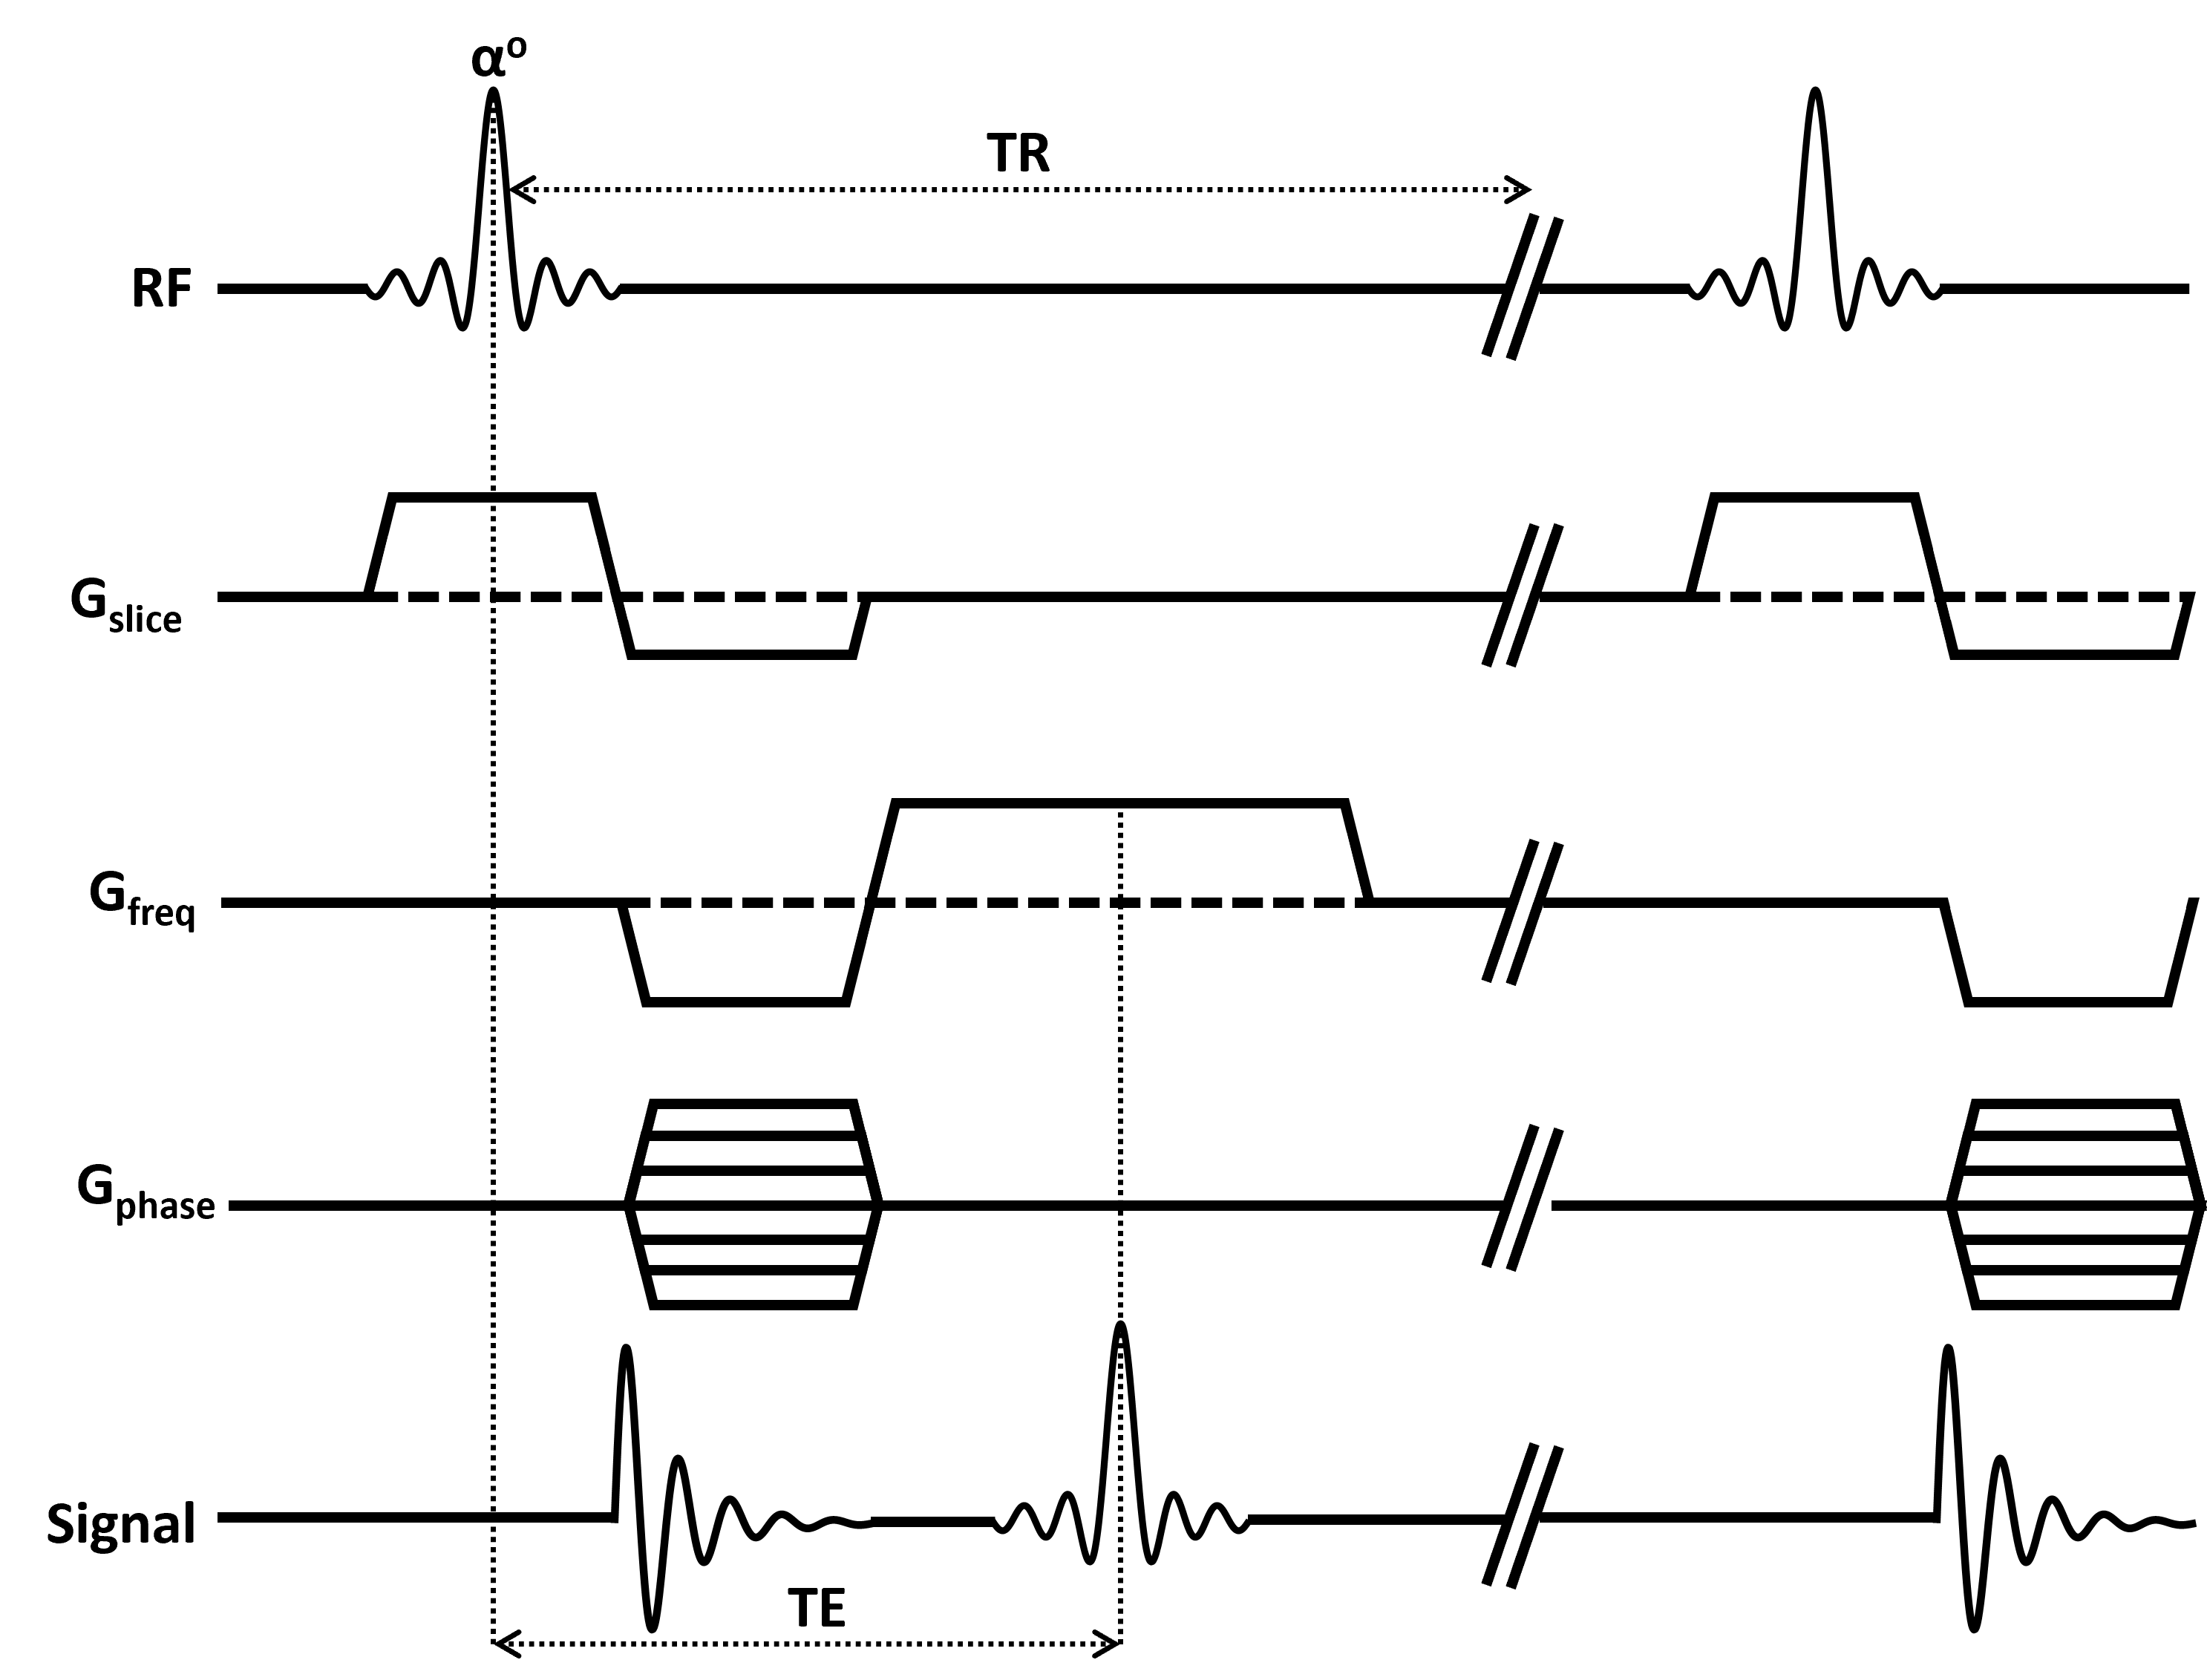
\includegraphics[width=0.8\textwidth]{Figures/Theory/GRE_sequence.png}
    \caption{\textit{Example pulse sequence diagram for a \ac{GE} imaging sequence, with the \ac{TE} indicated.}}
    \label{fig:theory:GRE}
\end{figure}

It has been shown the introduction of gradients can be used to acquire more spatial dimensions of an image. They can also be used to destroy/null signal in a specific region, for example it can be beneficial to null signal at the end of each \ac{TR} period. These gradients are referred to as `spoiler' gradients and work by de-phasing the transverse magnetisation spins. If signal can be nulled outside a 3D volume before imaging this can remove the need for slice selective gradients during imaging. This nulling is usually performed with the use of selective \ac{RF} pulses that excite magnetisation outside of the 3D volume, followed by the use of spoiler gradients. This is often referred to as \ac{OVS} and is commonly used to acquire reduced \ac{FOV} image data \cite{Smith2012ReducedSuppression}.

Longitudinal and transverse relaxation time constants vary depending on the type of tissue. Therefore, when a particular pulse sequence is used the choice of \ac{TR} and \ac{TE} will effect the the contrast in the image. The image signal in a \ac{GE} varies with flip-angle, \ac{TR} and \ac{TE} according to Eq. \ref{eqn:theory:Signal}, which drives the contrast.

\begin{equation}
    S = M_0\sin(\alpha)\exp(-\textrm{TE}/T_2^*)\frac{(1-\exp(\textrm{TR}/T_1)}{(1-\cos(\alpha)\exp(-\textrm{TR}/T_1))}
    \label{eqn:theory:Signal}
\end{equation}

\noindent There are three main types of contrast in an image: T$_1$-weighted, T$_2$-weighted and spin density weighted. The contrast in spin-density images comes from the difference in the density of spins in a particular tissue being emphasised. Remembering that most commonly the spin of interest is $^1$H, it is the $^1$H proton density that gives the contrast. The contrast in T$_2$-weighted images is emphasised by differences in T$_2$ times of different tissues, in order to produce these images long \ac{TR}s and long \ac{TE}s are used which minimises effects from different T$_1$s. Finally in T$_1$ weighted images the contrast is dominated by differences in the T$_1$ times of different tissues. This contrast is produced by choosing short \ac{TR}s and \ac{TE}s which minimise effects from different T$_2$ times. 

The \ac{SNR} obtained from a specific pulse sequence often depends on how quickly data can be acquired. One of the biggest aspects of scanning that affects the time taken is how data in k-space is obtained (k-space traversal). By traversing k-space more efficiently, scan time can be reduced which can make scanning more comfortable or can be used to improve \ac{SNR} by increasing the number of averages in a fixed scan duration. One of the biggest improvements in the traversing of k-space came with the development of \ac{EPI} \cite{Stehling1991Echo-planarSecond}.

\subsection{MRSI}

Acquiring MR spectra allows molecular concentrations to be obtained by comparing the magnitudes of peaks/signals at different chemical shifts, whilst MR images provide good contrast for structural differences. It is possible simultaneously to acquire information on chemical/molecular concentrations as well as structural information using a technique called \ac{MRSI}, which is effectively a combination of \ac{MRS} and MRI. This technique provides individual spectra from small volumes that are packed together into a 2D/3D grid that covers a larger volume/tissue. The voxels are often much larger than what would usually be acquired using \ac{MRI}, but maybe smaller than what would be acquired using \ac{MRS} strategies. By calculating concentrations for the visible molecules in each spectra the spatial distribution of each molecule can therefore be represented as a coarse image. This is often overlaid onto an anatomical image so that the corresponding regions can be easily identifiable. Concentration changes in specific tissues can therefore be used as bio-markers for disease. In order to obtain this type of data different pulse sequences that use different combinations of \ac{RF} pulses and gradients are used. 

\subsubsection{Chemical Shift Imaging}

\begin{figure}[h]
    \centering
    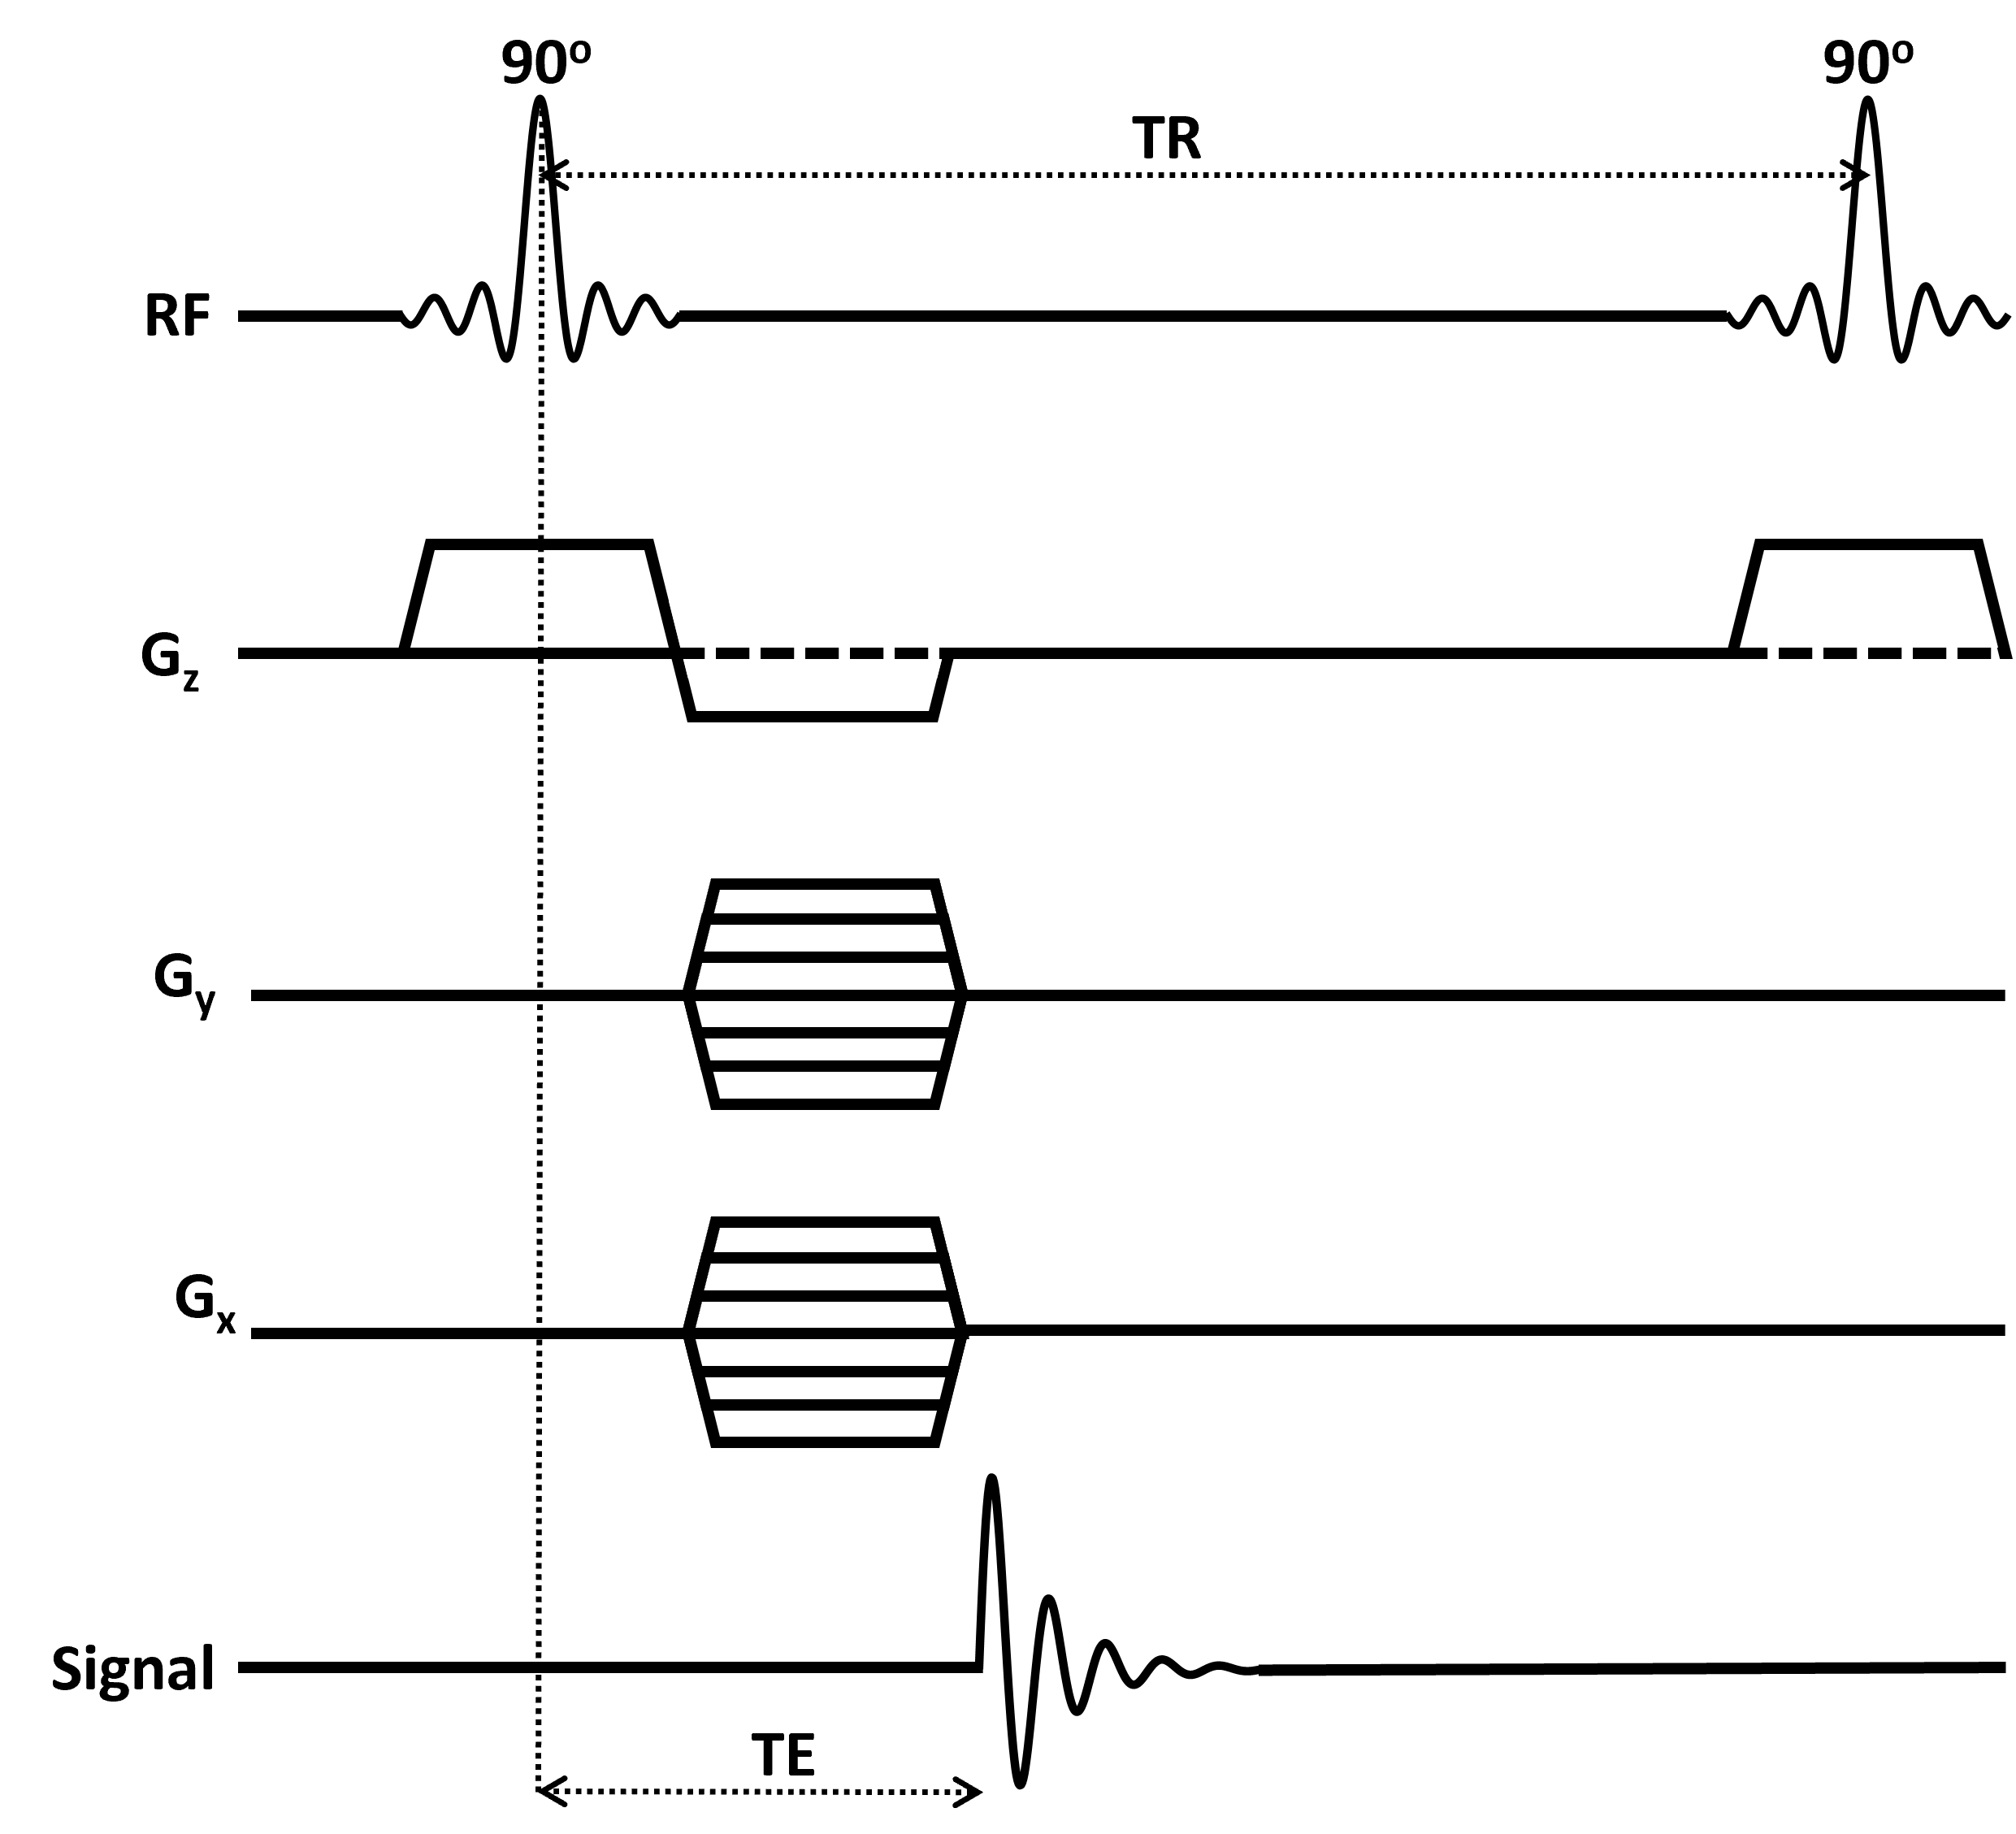
\includegraphics[width=0.9\textwidth]{Figures/Theory/CSI_sequence.png}
    \caption{\textit{Example pulse sequence diagram for a 2D \ac{CSI}, which includes a 90$^\circ$ \ac{RF} pulse applied at the same time as a slice selective G$_z$, which is followed by a rephasing lobe. During rephasing, G$_x$ and G$_y$ gradients are applied to spatially localise the resulting \ac{FID} which is also shown.}}
    \label{fig:theory:CSI}
\end{figure}

The simplest and quickest method to acquire a spectrum is to apply an \ac{RF} pulse in a static magnetic field and acquire data from the FID immediately after the pulse. Application of a gradient during the \ac{RF} excitation will localise the data from a specific slice in the body. Often this gradient is applied in the z-direction to localise the signal from a transverse slice through the body. However any direction of gradient can be used to excite a region. For example a sagittal or a coronal slice can be excited instead. The combination of gradients increases the number of dimensions in which spatial position can be localised, as has been shown with gradient echo imaging in Fig. \ref{fig:theory:GRE}. By applying three phase-encoded gradients in three orthorgonal directions that excite three slabs, their overlap excites a cuboid shape which forms a voxel. By then changing the strength of each gradient for each \ac{TR} a full 3D grid of \ac{FID}s are obtained which can form a 3D grid of spectra. This pulse sequence is called \ac{CSI}, a diagram of the pulse sequence used to acquire a 2D \ac{CSI} is shown in Fig. \ref{fig:theory:CSI}. 

% Therefore, by applying gradients in all three Cartesian directions simultaneously only data from a small voxel is excited, if data is acquired during the full length of an \ac{FID} that will only come from one small voxel. By iteratively changing the strengths of the adjacent voxels are excited eventually a full 2D/3D grid of spectra is obtained, this pulse sequence is called \ac{CSI}. 

\ac{CSI} has been used for different nuclei ($^{13}$C, $^{31}$P and $^2$H) to create maps that show the distribution of different metabolites. Acquiring this type of data takes a long time which can be a problem is functional data was to be acquired, which motivates work to decrease the acquisition time for \ac{MRSI} data.

% \subsubsection{EPSI and SSFP}

% One of the first approaches developed for decreasing the imaging time was the introduction of \ac{EPI}. In usual \ac{GE} imaging the position in k-space returns back to zero, \ac{EPI} takes advantage of the position in k-space after an echo instead of letting it return to zero. By using multiple echoes and the use of small gradients to slightly change the position in k-space an entire 2D image can be obtained. Therefore \ac{EPI} refers to the use of a single \ac{RF} excitation to obtain an entire 2D k-space data-set. This has been implemented in imaging since 1977 \cite{Mansfield1977Multi-planarEchoes}. \ac{EPI} can also be applied to \ac{MRSI} to reduce scan times. This comes in the form of a relatively new pulse sequence called \ac{EPSI} \cite{Mulkern2001EchoImaging}. Unfortunately in \ac{MRI} there are very few situations where a positive benefit comes without associated negatives. This is no different with \ac{EPSI} as there is a reduction in \ac{SNR} that is equivalent to the reduction in scan time. The most common way to recover this \ac{SNR} is to increase the number of averages of the scan, however in order to recover all of the \ac{SNR} the averages needed would make a typical \ac{EPSI} and \ac{CSI} scan take the same amount of time \cite{Mulkern2001EchoImaging}. This may at first seem like a wasted exercise, however in some fields the reduction in \ac{SNR} maybe worth the trade-off as it makes \ac{MRSI} much more clinically viable. Also, since the \ac{EPSI} sequence has much more components than \ac{CSI} such as the gradients and echoes, there is more opportunity for development which can then improve \ac{SNR}, spectral resolution and/or scanning time even further. It has been shown that the use of multiple echoes can increase the spatial resolution without adding extra scan time \cite{Furuyama2011Multi-echo-basedScanner}. This has also been shown (along with an increased temporal resolution) by using acquisition in a single excitation and using parallel imaging (also called \ac{SENSE}) \cite{Posse2009Single-shotImaging}. Because of this and the useful trade-off between scan time and SNR, \ac{EPSI} has been successfully implemented in \ac{HP} metabolic imaging \cite{Topping2020AcquisitionNuclei,Eldirdiri2018DevelopmentScanner} and using $^2$H in the liver \cite{Min2023Deuterium7T}.

% \begin{figure}
    % \centering
    % 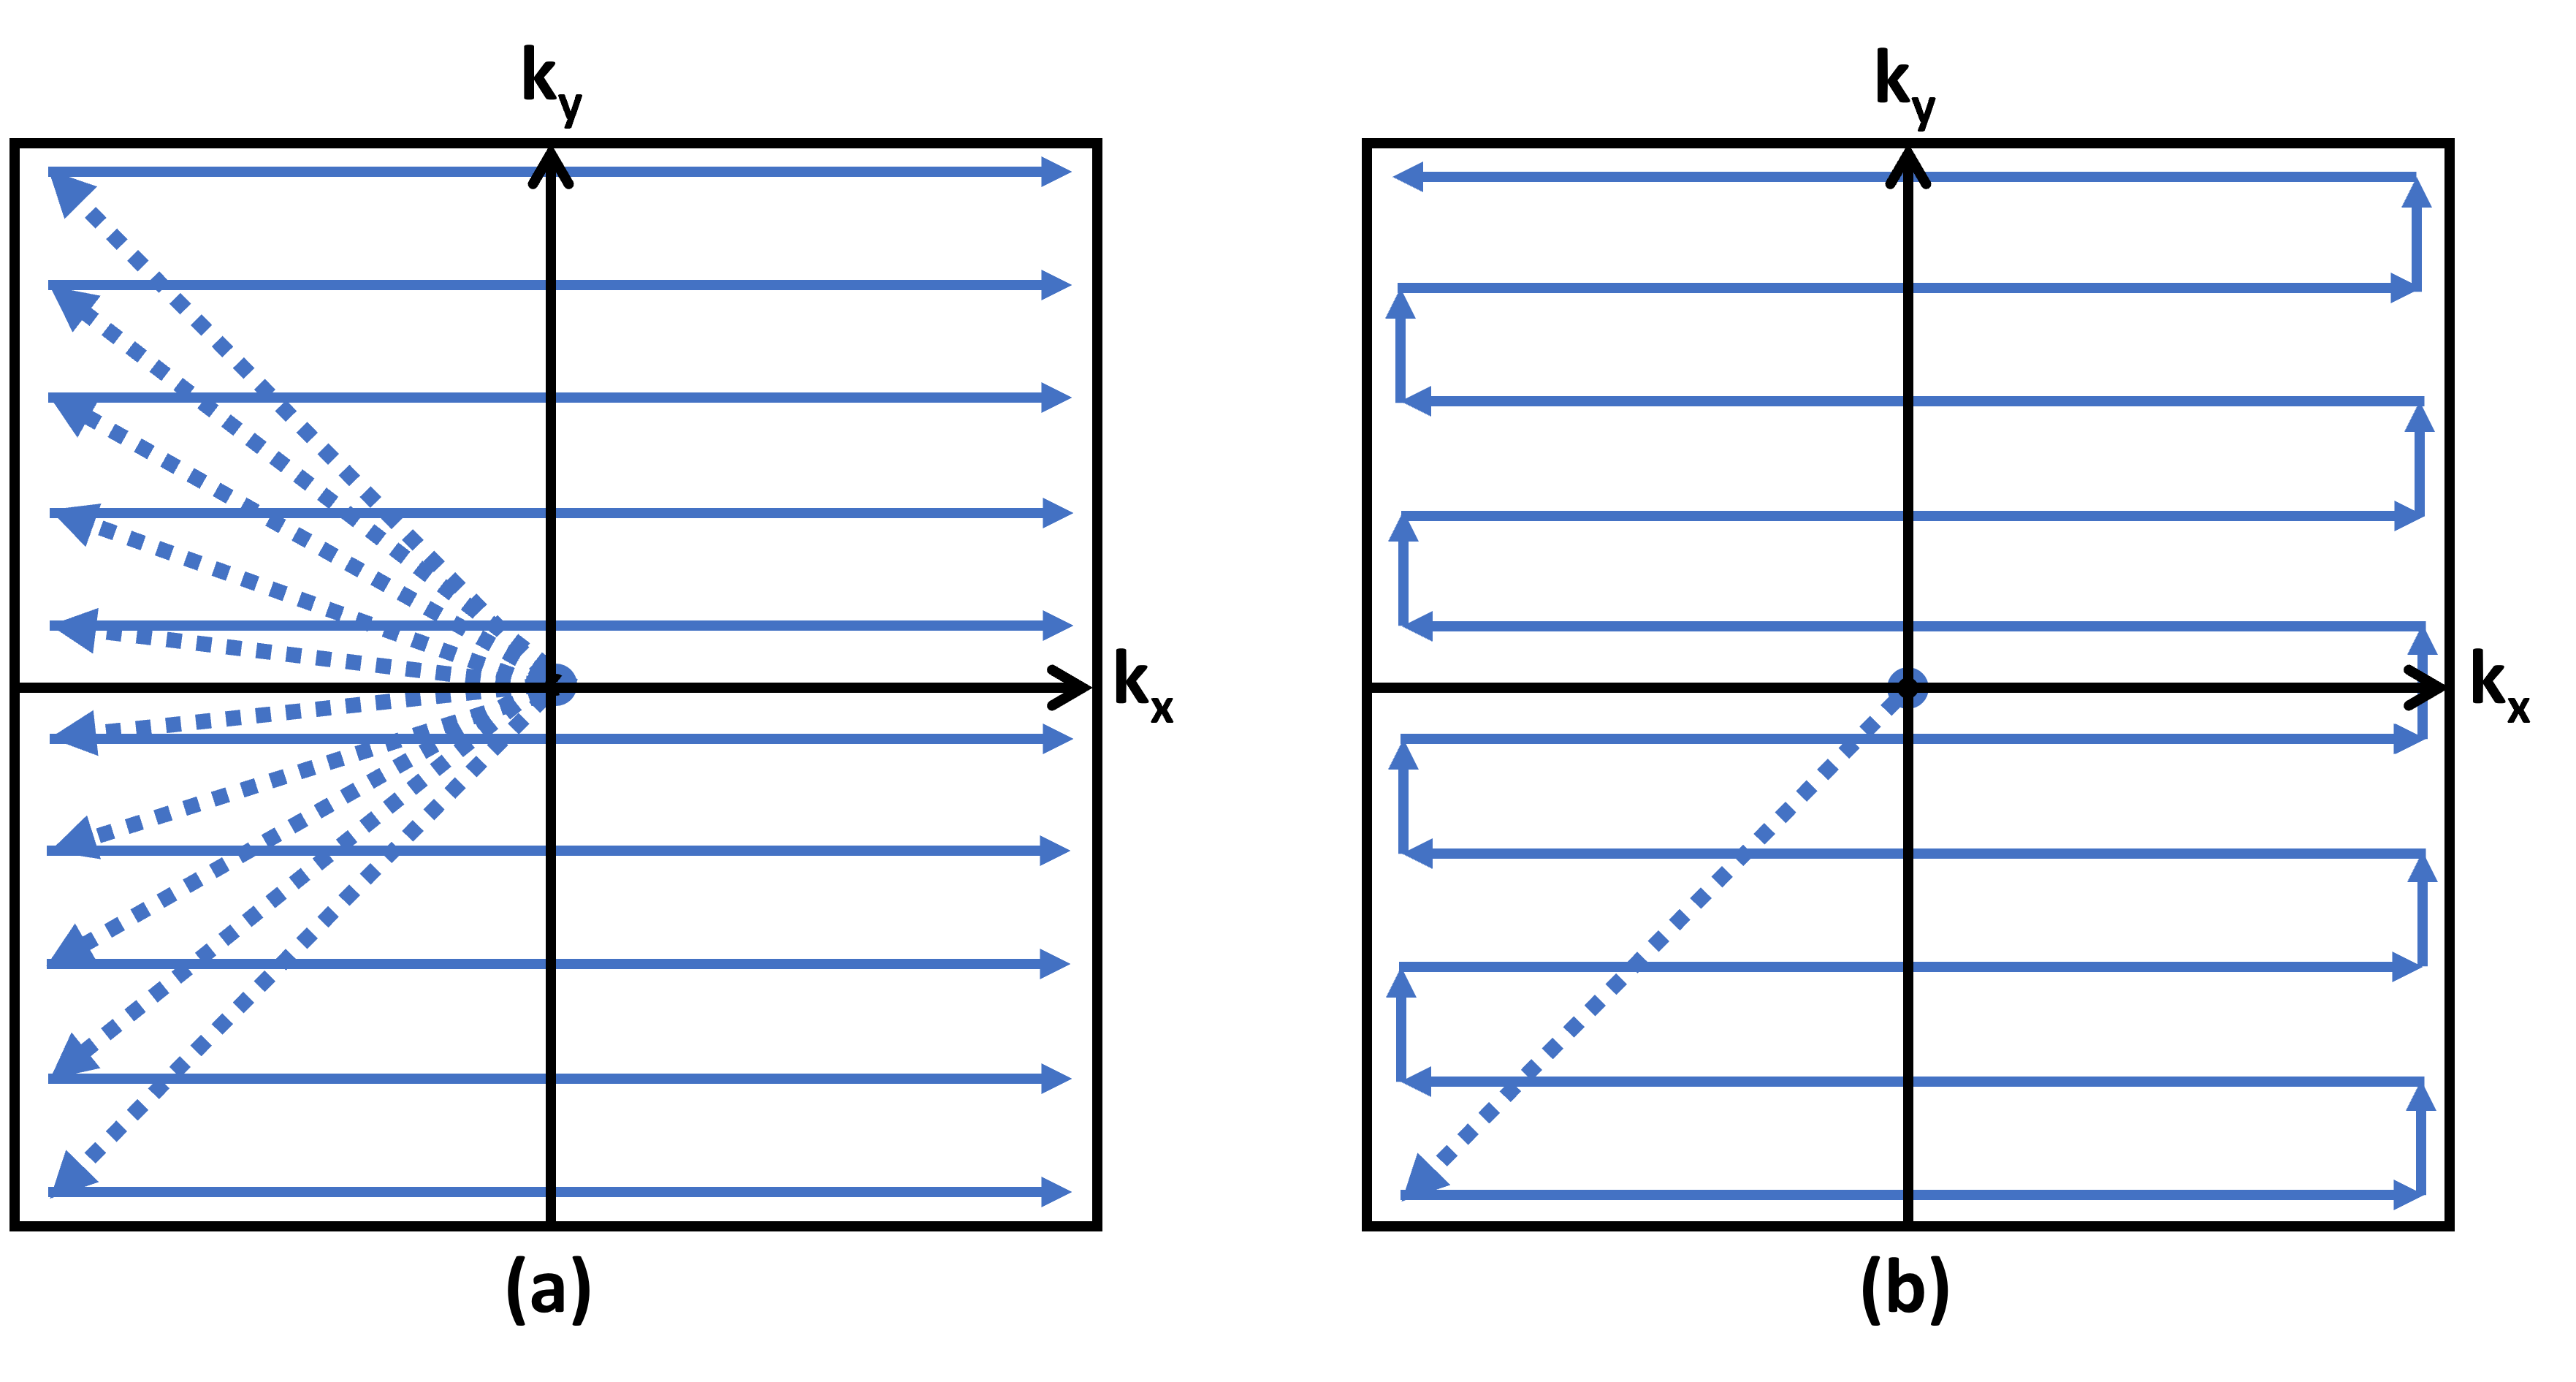
\includegraphics[width=0.9\textwidth]{Figures/Theory/kspace.png}
    % \caption{\textit{2D k-space traversal paths for a gradient-echo acquisition (a) and a echo-planar image acquisition.}}
    % \label{fig:theory:kspace}
% \end{figure}

% Balanced \ac{SSFP} \cite{Carr1954EffectsExperiments} is a special form of \ac{SSFP} where additional gradients are used to reduce off-resonance effects. \ac{SSFP} already known to increase \ac{SNR} compared to \ac{GE} imaging  \cite{Bieri2013FundamentalsMRI}, for situations where the T$_1$ to T$_2$ ratio is high (as \ac{SSFP} images have T$_1$/T$_2$ contrast). By using \ac{ME} \ac{SSFP}, with varying echo-times, it is possible to achieve good spectral separation of signals from the different metabolites, as the phase evolution between the metabolites across echoes will be different. So by combining the images for each echo as a non-linear problem using the IDEAL framework \cite{Reeder2007Water-fatImaging} metabolite maps, that appear similar to those acquired using \ac{CSI}, can be acquired. In doing this the \ac{SNR} enhancement of \ac{SSFP} is still maintained \cite{Peters2021ImprovingInvestigation}. The problem in doing this is the \ac{SNR} of this method will be higher for larger field strengths as the long echo-train needed to achieve phase separation of the different metabolite signals means that \ac{TR} is now too long to achieve sufficient \ac{SNR} gain (\ac{TR} $<<$ T$_1$ and T$_2$), this means the possible \ac{SNR} gain at lower field strengths needs to be explored. This has also only been performed for three different metabolites whereas this realistically needs to be able to analyse more metabolites which becomes much more complex. An alternative way of acquiring/analysing \ac{SSFP} data with spectrally separate metabolites is to alter the phase steps between successive \ac{RF} pulses in scans instead of the echo time, as it is much easier to separate multiple resonances and still keeps the \ac{SNR} increases of \ac{SSFP} which has been done using $^{13}$C \cite{Varma2016SelectiveSSFP}.

\section{Analysis}

\subsection{Quantification of MRS data}

When analysing \ac{MRS} data it is important to be able to accurately track changes for each spectra. The oldest method of doing this is peak integration whereby the spectral points spanning a peak are summed together. An integration range of at least two \ac{FWHM}'s wide is usually enough to obtain accurate quantification \cite{Near2021PreprocessingRecommendations}. The spectral peak integration value can also be obtained from the time-domain signal as the first point in the absorption spectra, as well as from the product of the \ac{FWHM}, $\pi$ and the spectral peak-height in the frequency domain \cite{deGraaf2019InSpectroscopy}. This technique is simple to implement computationally and takes little time, however it requires correctly phased spectra as any incorrect phasing will give the incorrect amplitude. Most biological tissues and processes involve complex chemical environments with many different compounds which will produce different MR signals appearing at different frequencies (also known as chemical shifts). This does not necessarily effect the peak integration method as long as each peak/signal has a large enough frequency offset relative to each other. However this is commonly not the case especially in $^1$H spectroscopy \cite{Alger2010QuantitativeReview}. 

Therefore, a different methodology is needed to overcome this issue, which comes in the form of fitting spectral signals to lineshapes, such as Lorentzian \cite{Lorentz1895TheHeat}, Gaussian and Voigt \cite{Near2021PreprocessingRecommendations} lineshapes. This fitting is often performed through a method called least-squares \cite{Golub1973TheSeparate} fitting whereby the sum ($R^2$) of the squared differences between the experimental data and a model (residuals) is minimised \cite{Vanhamme2001MRMethods}. Mathematically this is demonstrated in Eq. \ref{eqn:theory:LS}.

\begin{equation}
    R^2 = \sum_{i=1}^{n}[y_i - f(x_i,a_1,a_2,...,a_n)]
    \label{eqn:theory:LS}
\end{equation}

\noindent Where $i$ represents each data point with $n$ data points, and the range of values $a_1$ to $a_n$ covers the amount of fitting parameters such as linewidth (similar to \ac{FWHM}), frequency position, phase and most importantly amplitude. $R^2$ is said to be minimised when the following differential relationship for each fitting parameter is met, in Eq. \ref{eqn:theory:Diff} the derivative is referred to as the Jacobian.

\begin{equation}
    \frac{\partial (R^2)}{\partial a_i} = 0
    \label{eqn:theory:Diff}
\end{equation}

\noindent The fitting begins by using initial parameter guesses and finds the sum of squared residuals. An optimisation algorithm is then used to update the parameter values iteratively, until a certain threshold in the $R^2$ value is met or the max number of iterations is reached. The best way to model experimental \ac{MRS} data is in the time domain as a series of exponentially damped sinusoids. 

Since the full spectra comprises the sum of many individual damped sinusoids. The more signals present in the spectra the more difficult computationally this becomes. There is consequently a strong motivation to reduce the number of parameters, reduce the computational load and therefore increase the reliability of the fitting \cite{Near2021PreprocessingRecommendations}. It has been shown that one way to improve the reliability of fitting spectra that suffer from overlapping signals, which is the case for $^{31}$P \ac{MRS} data, is to use prior knowledge \cite{Hamilton2003PriorSpectra}. Some of the overlapping signals while distinctly different can share common ratios between some of their fitted parameter. One of the first fitting algorithms to include prior knowledge was the \ac{VARPRO} method \cite{Golub1973TheSeparate} which has successfully been used to analyse $^{31}$P data \cite{vanderVeen1988AccurateKnowledge,Stubbs199631P-MagneticADP}. Whilst \ac{VARPRO} was successful as an improved fitting methodology, a new technique was recently developed called \ac{AMARES} which fits more reliably and accurately, as well as having increased functionality, including lineshape choice, fitting of echo signals and imposition of upper and lower bounds on fitting parameters \cite{Vanhamme1997ImprovedKnowledge}. \ac{AMARES} is used regularly in \ac{MRS} analysis and is included in software packages such as JMRUI \cite{Stefan2009QuantitationPackage} and OXSA \cite{Purvis2017OXSA:MATLAB}, which have previously been used to analyse $^2$H \ac{MRS} data \cite{Simoes2022GlucoseGlioblastoma,Kreis2020MeasuringMRI,Kaggie2022DeuteriumMetabolism}. The model of summed damped sinusoids that is used in the \ac{AMARES} package is mathematically shown in Eq. \ref{eqn:theory:model}, with the trust region-reflective optimisation algorithm.

\begin{equation}
    y_n = \hat{y_n} + e_n = \sum_{k=1}^{k}a_k\exp(i\phi_k)\exp(-d_k(1-g_k+g_kt_n)t_n)\exp(i2\pi f_kt_n) + e_n
    \label{eqn:theory:model}
\end{equation}

\noindent Here $k$ is the number of sinusoids, $\phi_k$ is the phase, $d_k$ is the damping factor, $g_k$ determines the lineshape (1 for Gaussian, 0 for Lorentzian), $t_n$ is the time for each point, $f_k$ is the frequency offset and $e_n$ describes complex white Gaussian noise. The caret indicates the model as opposed to actual measurement.

Even \ac{AMARES} has its limits and signal fitting can struggle when many peaks are present especially in terms of overlapping signals, which can be a big problem in $^1$H \ac{MRS} data. Therefore, a new methodology was developed to overcome this called linear combination and was made into a toolbox that is called LCModel \cite{Provencher1993EstimationSpectra}. This works by fitting total spectra for each metabolite (called basis sets) instead of individual peaks, this reduces the number of model parameters and leads to increased reliability in fitting. The basis sets can be acquired by either phantom \textit{in vitro} experiments or by numerical simulation \cite{Near2021PreprocessingRecommendations}. Because of this it is more complicated to set up so it is yet to be used commonly for the more simplified and sparse spectra from $^{13}$C, $^{31}$P and $^2$H, although it has been used in analysing data for the indirect detection of $^2$H glucose by looking at the loss in $^1$H signal \cite{Rich20201HVivo,Cember2022IntegratingHumans,Niess2023Reproducibility3T}. 

\subsection{Post-Processing Improvement of SNR}

The low \ac{SNR} of $^2$H is often a problem during scanning and as scanning times have to be kept short for participant/patient comfort this can be a problem in spectroscopy with any nuclei. Whilst fitting in the frequency domain can provide accurate fitting and quantification, it is now common practice to fit data in the time-domain which can have the ability to provide more accurate and reliable fitting \cite{Joliot1991InMethods}. In order to increase the reliability and reproducibility of values obtained from analysis it is important to maximise the \ac{SNR}. A popular method of increasing the \ac{SNR} of spectra is to apply spectral filtering in the form of apodisation. Common lineshapes that are used in the filtering are exponential and Gaussian \cite{Goryawala2020EffectsFitting}. Applying a Gaussian filter can reduce the \ac{FWHM} of MR signals which can improve fitting reliability however this will also change the lineshape of the signal, the best way to do this is to apply an exponential filter along with a Gaussian to negate the previous lineshape such that the new signal shows only a Gaussian linseshape. However, it has been shown that apodisation can reduce accuracy of fitting especially in cases of complex spectra where signals overlap spectrally \cite{Bartha1999FactorsFiltering}. As a result, apodisation is often used sparingly and often only used for visual demonstrations of data. Lots of alternatives exist in terms of denoising including \ac{PCA} \cite{Abdoli2016DenoisingComponents} and low rank approximation \cite{Nguyen2013DenoisingApproximations} that have been shown to provide improved \ac{SNR} without limiting quantification \cite{Clarke2022UncertaintyMethods}. 

\ac{SVD} is a linear algebra technique that breaks down a 2D matrix into its key components, and is used to reduce a matrix without affecting the data. An example would be a 2D matrix $A$ that is $m$ x $n$ in size will have $m$ x $n$ values, if this can be decomposed into two vectors that are orthogonal such that $A$ = $\mathbf{uv}^\textrm{T}$ the total number of values in these vectors is $m+n$. Therefore large data sets can be compressed into sent a smaller storage size without compromising the data itself. The \ac{SVD} starts off originally as an eigenvalue  problem with $\sigma$ representing the eigenvalue while $u$ and $v$ are eigenvectors. The eigenvalue problem only works when $A$ is a square matrix, if $A$ is a rectangular matrix with $m$ x $n$ size the eigenvectors become square matrices with sizes $m$ x $m$, $U$ and $n$ x $n$ $V$. Here each column of $v$ and each row of $u$ diagonalizes the matrix $A$ similar to an eigenvalue problem.

\begin{equation}
    A \mathbf{v}_n = \sigma_r \mathbf{u}_m ,
\end{equation}

\noindent where $r$ is the `rank' of the matrix and contains all the key components of $A$. The eigenvalues then form the diagonal elements of the matrix $\Sigma$ called the `core matrix', the eigenvalues are called the singular values and the size represents the importance for reconstructing $A$. By rearranging the matrices Eq. \ref{eqn:theory:SVD} is created for the matrix $A$.

\begin{equation}
    A = U\Sigma V^\textrm{T} = \sum_{k=1}^{r} u_k\sigma_kv_k^\textrm{T}
    \label{eqn:theory:SVD}
\end{equation}

\noindent However, a full reconstruction does not necessarily need to be performed, if the core matrix is arranged by size and the lower singular values are removed, $A$ can be reconstructed using only the more important features. When this technique is applied to \ac{MRS} data this will de-noise the data as the noise will be represented by the lower singular values \cite{Brender2019DynamicHyperpolarization}. This technique can also be also used to fit \ac{MRS} data, as the results can be converted into the regular fitting parameters \cite{Pijnappel1992SVD-basedSignals}, as well as to remove water signal in post-processing \cite{Cabanes2001OptimizationBrain}.

This approach only works with 2D matrices, which is an issue for \ac{MRSI} data which commonly has up to five dimensions (one spectral, three spatial, and a temporal domain). However, a similar technique can be used when more dimensions are present called \ac{HOSVD}. This is similar to regular \ac{SVD} but has the ability to work with higher dimension data. Here the matrix is decomposed into a collection of tensors $U$ equal to the number of dimensions of $A$ which is $d$, along with a core tensor $S$. The mathematical form of this decomposition is shown in Eq. \ref{eqn:theory:HOSVD}.

\begin{equation}
    A = S \otimes U_1 \otimes U_2 \otimes ... \otimes U_d
    \label{eqn:theory:HOSVD}
\end{equation}

\noindent This gives a core tensor that is the same size in each dimension, which can be truncated in a similar way to \ac{SVD}, so that when the original matrix $A$ is reconstructed the less important components are removed. For \ac{MRSI} data this de-noises the data as the lower singular values again represent the noise. The core tensor here will have the same size in each dimension, which is not optimal for \ac{MRSI} data as often the spectral dimension will be much larger than the spatial or temporal dimensions. To overcome this a Tucker decomposition is used which allows a core tensor of any size to be constructed \cite{Tucker1966SomeAnalysis}, this gives much more control over the level of de-noising that is applied. This whole method is called a Tucker-Tensor decomposition and it has been used previously to de-noise \ac{DMI} data \cite{Kreis2020MeasuringMRI, Assmann2020InCholesterol}. This strategy has been implemented in this work using a MATLAB toolbox \cite{Bader2007EfficientTensors}.

% \subsection{Concentration Calculation} % Potential
% Robins section from glucose paper 

\section{RF Coils}

\ac{RF} coils have two functions: first to apply a B$_1$ field to tip the magnetisation, and second to receive a signal from precessing magnetisation Faraday's law of induction. The profile of the applied B$_1$ field depends on the design/shape of the coil, the sensitivity of the coil also depends on the electronic components used for tuning and matching. The frequency of the applied $B_1$ depends on the applied waveform. The key point in designing/building the \ac{RF} coil is to maximise the $B_1$ per unit voltage by tuning the coil to resonate at the Larmor frequency and matching the coil's impedance to whatever it is connected to. This shows how important design and building of \ac{RF} coils is. Lots of different companies exist from whom it is possible to buy \ac{RF} coils. This can be expensive due to the experience and time that goes into coil building. Therefore it is useful when starting new research with a new nucleus of interest (such as $^2$H) to be able to build home-made coils. 

\subsection{Theory}

% the voltage and current and the relationship with phase can be demonstrated through a phasor diagram which can also represent complex numbers. Therefore, many electrical components can also be represented as complex numbers. The current variation with time ($I(t)$) of an RLC circuit is shown in Eq. \ref{eqn:theory:Current}.

% \begin{equation}
    % I(t) = I_{\mathrm{max}}\sin(\omega t + \phi)
    % \label{eqn:theory:Current}
% \end{equation}

% According to Ohm's law the voltage across a resistor ($\Delta V_R$) can be found, an inductor will oppose the current and will therefore have a corresponding reactance ($X_L$) and will be 90$^\circ$ ahead of the current. The time-varying voltage will cause the capacitor to continuously charge and discharge which resists the change in voltage and will also have a reactance ($X_C$). 

The simplest way to build an \ac{RF} coil is to shape a wire into a loop (inductor) and connect a capacitor in parallel. This forms what is known as an LCR circuit which is often used to create a resonance. The LCR circuit will have a natural resonance frequency ($\omega_0$), therefore when the frequency of the applied voltage is the same as this natural frequency the circuit is considered on resonance ($\omega=\omega_0$). For a circuit to resonate reactance ($X$), needs to be minimised. $X$ is the imaginary component of the impedance given as $Z = R+iX$, and for an LCR circuit is composed of two components the inductive reactance ($X_L$) and the capacitive reactance ($X_C$). The total reactance for a series LCR is the difference between $X_L$ and $X_C$, for a parallel LCR circuit the reciprocal of the total reactance is equal to the sum of the reciprocal of the individual components. The relationship between the reactances and the resonant frequency is shown in Eq. \ref{eqn:theory:X}.

\begin{equation}
\begin{gathered}
    X_L = i\omega L \\
    X_C = \frac{1}{i\omega C}
    \label{eqn:theory:X}
\end{gathered}
\end{equation}

The resonant condition of the LCR circuit is then well demonstrated by calculating the current flow, which is shown in Eq. \ref{eqn:theory:I} as the ratio between the voltage and the impedance.

\begin{equation}
    |I| = \left| \frac{V}{Z} \right| = \left| \frac{V}{R+i(\omega L - \frac{1}{\omega C})} \right| = \left| \frac{V}{\sqrt{R^2+(\omega L - \frac{1}{\omega C})^2}} \right|
    \label{eqn:theory:I}
\end{equation}

The natural resonance of the circuit is therefore given in Eq. \ref{eqn:theory:res}.

\begin{equation}
    \omega_0 = \frac{1}{\sqrt{LC}}
    \label{eqn:theory:res}
\end{equation}

The voltage variations with time for each electrical component are shown below in Eq. \ref{eqn:theory:Voltage}. As an \ac{RF} $B_1$ field is applied to the coil, current will be induced which charges the capacitor. As the $B_1$ is then reduced, the capacitor will then release stored energy which causes current to flow through the rest of the circuit. Energy is dissipated in the resistor and therefore the current decreases exponentially. Graphs of the change in voltage in this case are shown in Fig. \ref{fig:theory:VI}, along with the corresponding absorption and dispersion curves. This behaviour is often referred to as a driven resonance.

\begin{equation}
\begin{gathered}
    \Delta V_R = IR = I_{\mathrm{max}}R\sin(\omega t + \phi) \\
    \Delta V_L = \omega LI_{\mathrm{max}}\cos(\omega t + \phi) =  X_LI_{\mathrm{max}}\cos(\omega t + \phi)\\
    \Delta V_C = -\frac{I_{\mathrm{max}}}{\omega C}\cos(\omega t + \phi) = -X_C\cos(\omega t + \phi)\\
    \label{eqn:theory:Voltage}
\end{gathered}
\end{equation}

If the time in which the driven resonance is applied is short the overall behaviour is the impulse response. The most common cables that are used to connect to \ac{RF} coils are coaxial cables, which usually have a characteristic impedance of 50 $\Omega$. When a coil is constructed and tuned to the Larmor frequency the impedance is most likely different to the impedance of the cable. The difference in impedance will cause some of the power to be reflected at the coil instead of transmitted. Therefore, the impedance of of the coil needs to be changed, which can be done by changing its reactance. The most common ways of doing this are by adding an inductor or a capacitor in parallel with the coil. The method of adding a capacitor will be discussed here and an example circuit can be seen in Fig. \ref{fig:theory:RLC}.

\begin{figure}
    \centering
    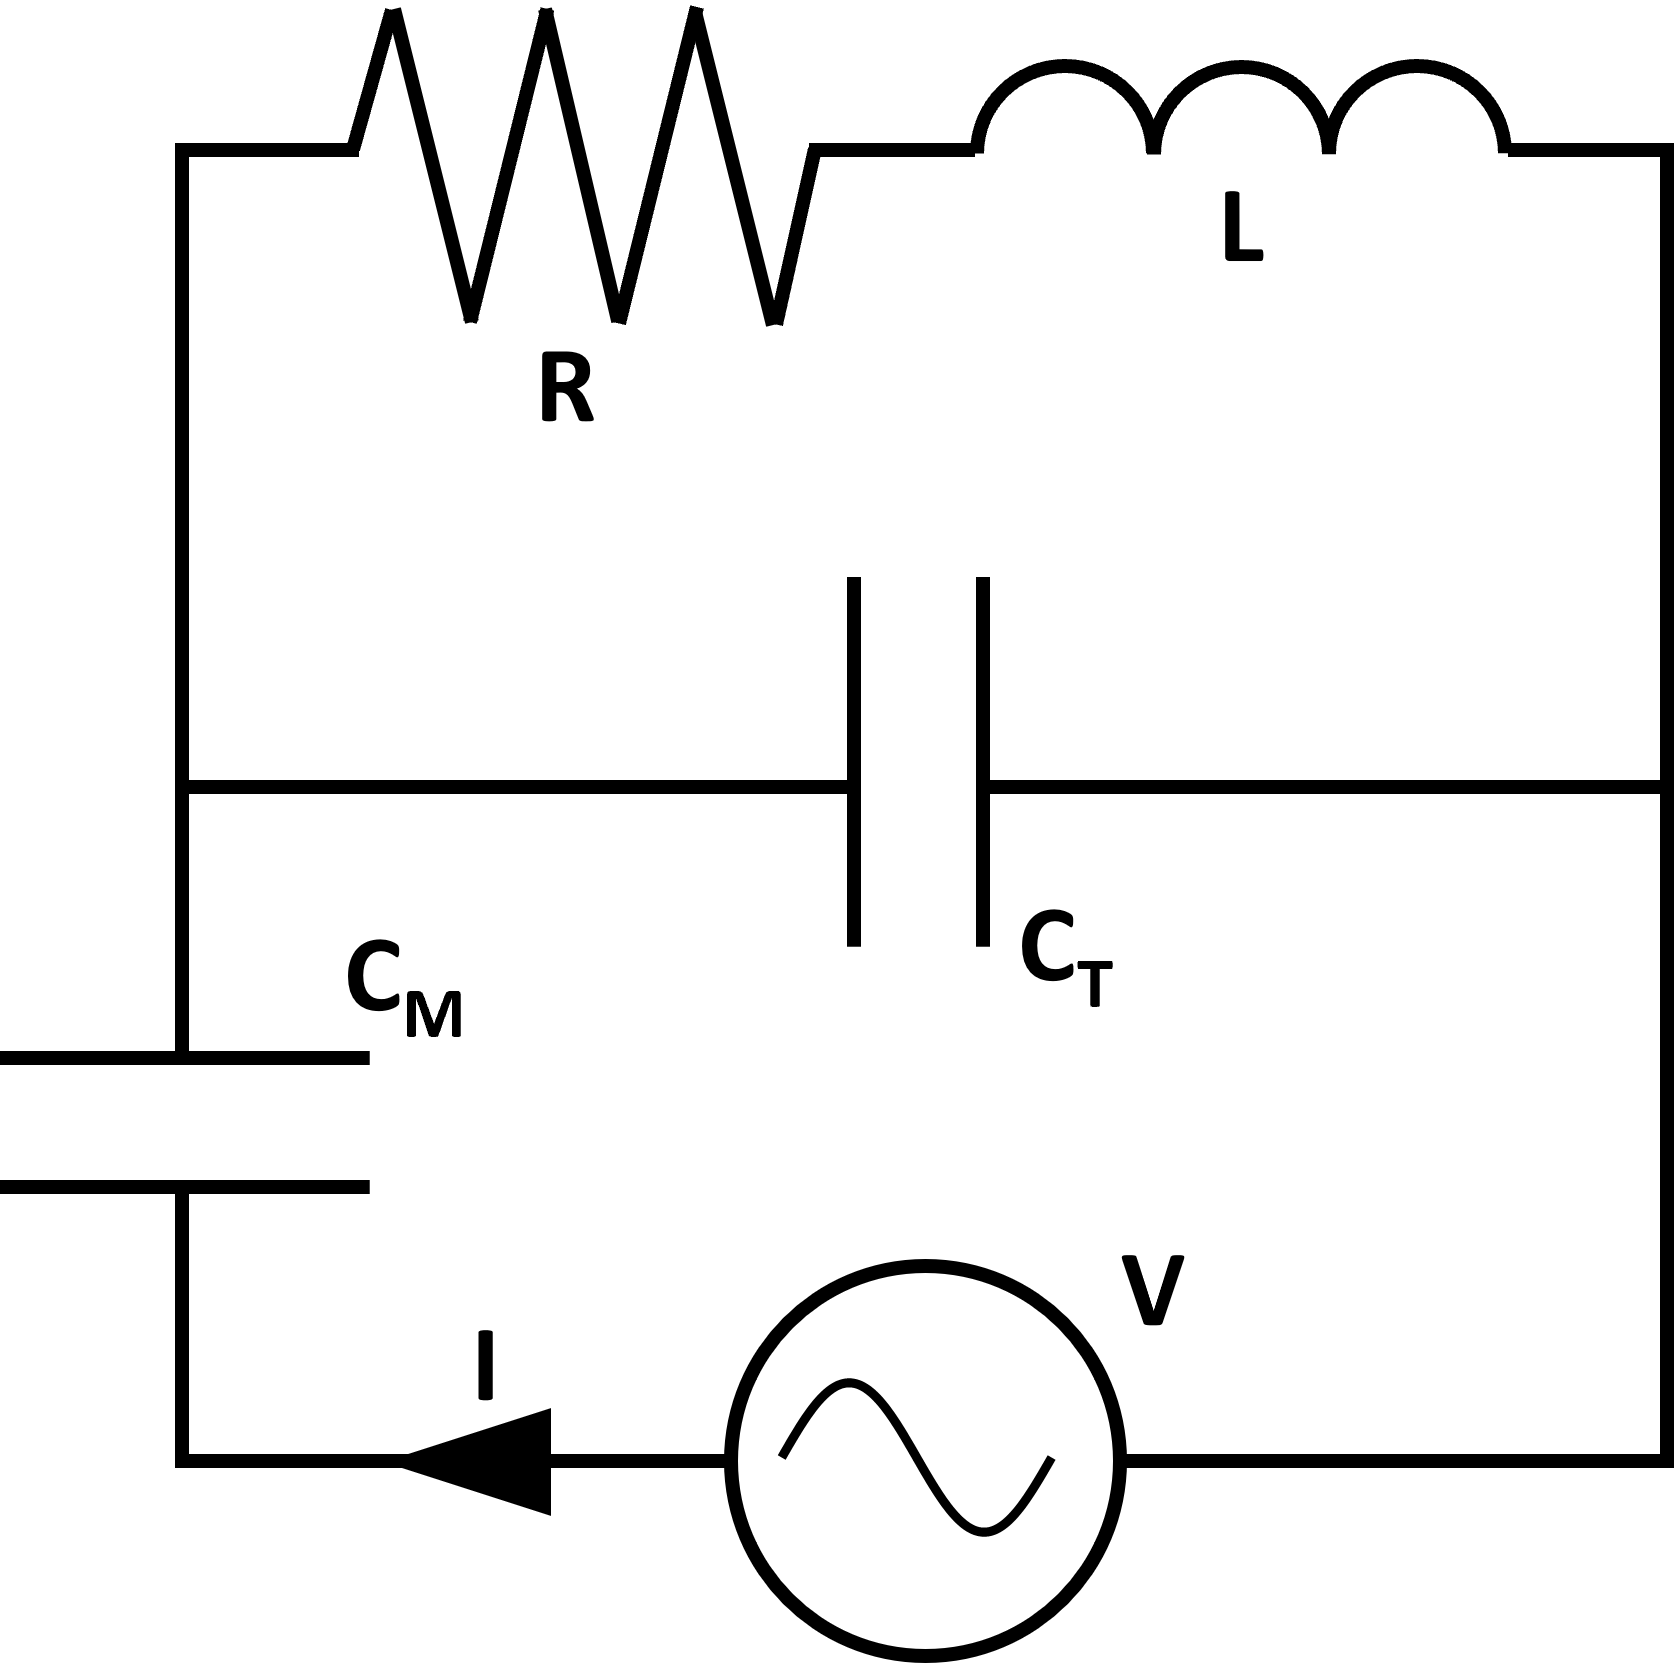
\includegraphics[width=0.6\textwidth]{Figures/Theory/RLC_Circuit.png}
    \caption{\textit{Example diagram of an LCR circuit with both tuning (C$_T$) and matching capacitors (C$_M$), along with an AC signal generator.}}
    \label{fig:theory:RLC}
\end{figure}

The capacitor in series with the coil is referred to as the tuning capacitor (C$_T$) with the other capacitor called the matching capacitor (C$_M$). The total capacitance is C$_M$+C$_T$. A relationship between C$_M$ and C$_T$ can be found that is related to the quality factor (Q) \cite{Chen1989ChapterNoise} which is the resonance frequency divided by the bandwidth of the coil resonance in Fig. \ref{fig:theory:VI}, and is shown in Eq. \ref{eqn:theory:match}. 

\begin{equation}
    C_M = \sqrt{\frac{C_T}{Q\omega_0Z}}
    \label{eqn:theory:match}
\end{equation}

The combination of Eqs. \ref{eqn:theory:res} and \ref{eqn:theory:match} can be used to find the capacitances needed to tune and match the coil \cite{Chen1989ChapterNoise}. To test a fully constructed coil an \ac{AC} is applied to the coil and the reflected power is plotted against frequency as a logarithmic scale measured in decibels (dB), the graph will appear similar to the absorption spectra shown in Fig. \ref{fig:theory:VI}. A level of 20 dB is commonly perceived as a good enough value of reflected power, with the peak appearing at the Larmor frequency. Realistically soldering and adding components will change the circuit and the theoretical components can be wrong so will often need changing based on the measured response.

\begin{figure}
    \centering
    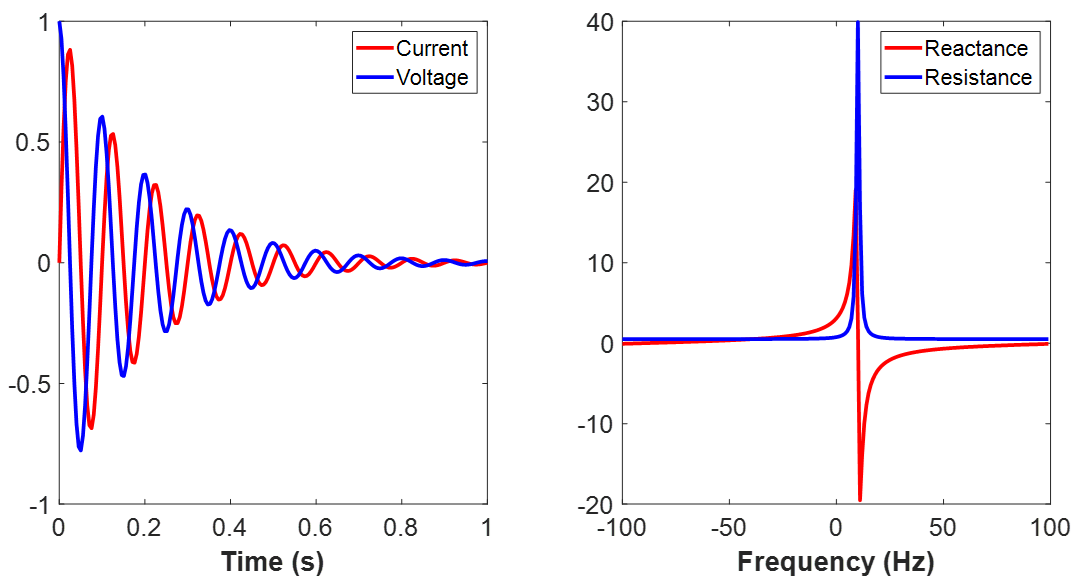
\includegraphics[width=0.9\textwidth]{Figures/Theory/VI.png}
    \caption{\textit{(a) Current and Voltage graphs for a dissipating capacitor in an RLC circuit. (b) Impedance variation with frequency which demonstrate the resistive and reactive components.}}
    \label{fig:theory:VI}
\end{figure}

When a coil is placed over a sample or body tissue coupling occurs which changes the total impedance. This can change the matching condition as well as the resonant frequency of the coil. Therefore it is important to load the coil with a phantom that matches the loading response that will be present during scanning, when designing/building the coil. 

\subsection{Coils Built}

Three different coil types were constructed for use in the experiments reported here and implemented for use on a Philips 3T Achieva system. These were two surface coils, a saddle coil and a Helmholtz coil. All coils were tuned to 19.6 MHz, the Larmor frequency of $^2$H at 3T. A 2 litre salt-water solution was used to load each coil, since each coil was used for scanning on different body parts the loading response changed slightly which was controlled by changing the salt concentration. A birdcage coil dual tuned to the Larmor frequencies of $^1$H and $^2$H at 7T was purchased from Rapid Biomedical for use on a 7T Philips Achieva System. The in-house built coils were used to acquire spectroscopic $^2$H data with anatomical $^1$H images being acquired using the whole-body \ac{RF} coil in the scanner for transmission and reception. The purchased coil is able to acquire $^1$H anatomical images as well as $^2$H spectroscopic data, low resolution $^2$H images were also acquired using this coil.

\subsubsection{Surface Coil}
\label{Chap:Theory:Coils}

A surface coil is the simplest and most basic coil to design, where the coil often forms a simple circular loop. The magnetic field is largest on axis and decreases, with distance from the coil. Therefore the field is spatially inhomogeneous which is why this coil design is often used for non-localised spectroscopy, where the localisation of the signal is down to the placement of the coil. The penetration depth of the magnetic field for a surface coil is approximately equal to the diameter of the coil \cite{Gruber2018RFNonphysicists}, and therefore a surface coil is sensitive to regions closest to the coil. 

\begin{figure}
    \centering
    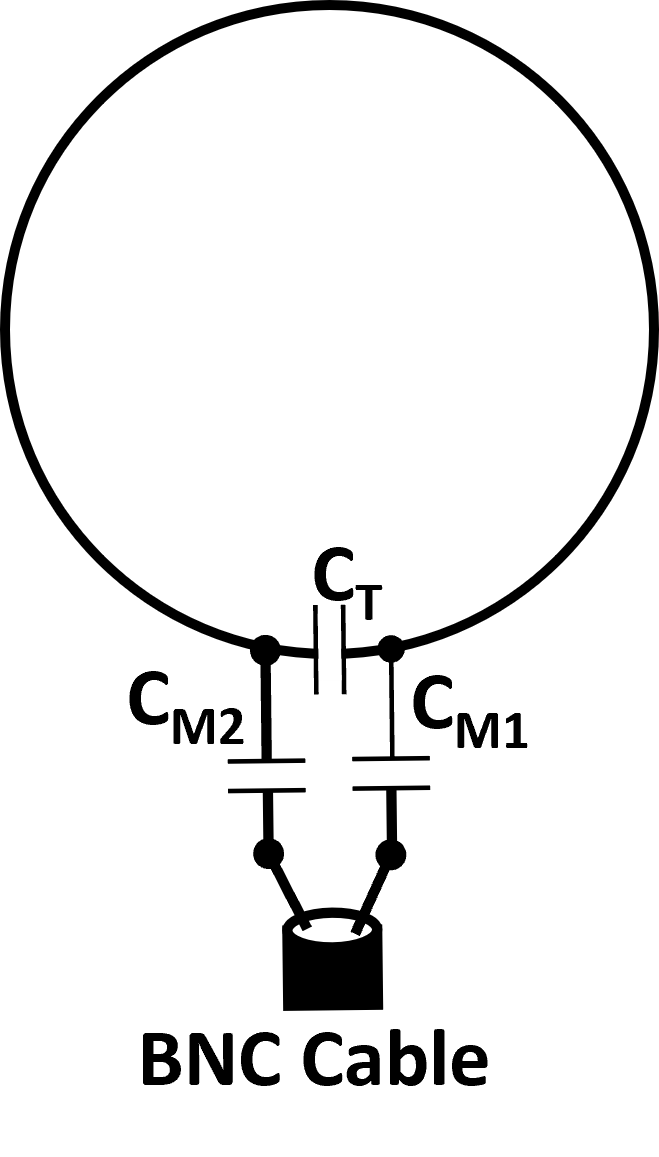
\includegraphics[width=0.3\textwidth]{Figures/Theory/Surface_Coil.png}
    \caption{\textit{Diagram of a typical planar surface coil with circuit elements attached, the coaxial cable attaches to a BNC connector. C$_T$ is the tuning capacitor and C$_{M2}$ and C$_{M1}$ are the matching capacitors.}}
    \label{fig:theory:Surface}
\end{figure}

The surface coils used for data collection were built for use in the study described in Chapter \ref{Chap:Lipid}. The first coil is a small 5 cm coil with two loops of copper wire with a tuning capacitance of 173.4 pF and a matching capacitance of 11 pF which is split over both wires of the loop to keep it balanced. The coil is made small to maximise the sensitivity to signal from subcutaneous fat in the calf.

\begin{figure}
    \centering
    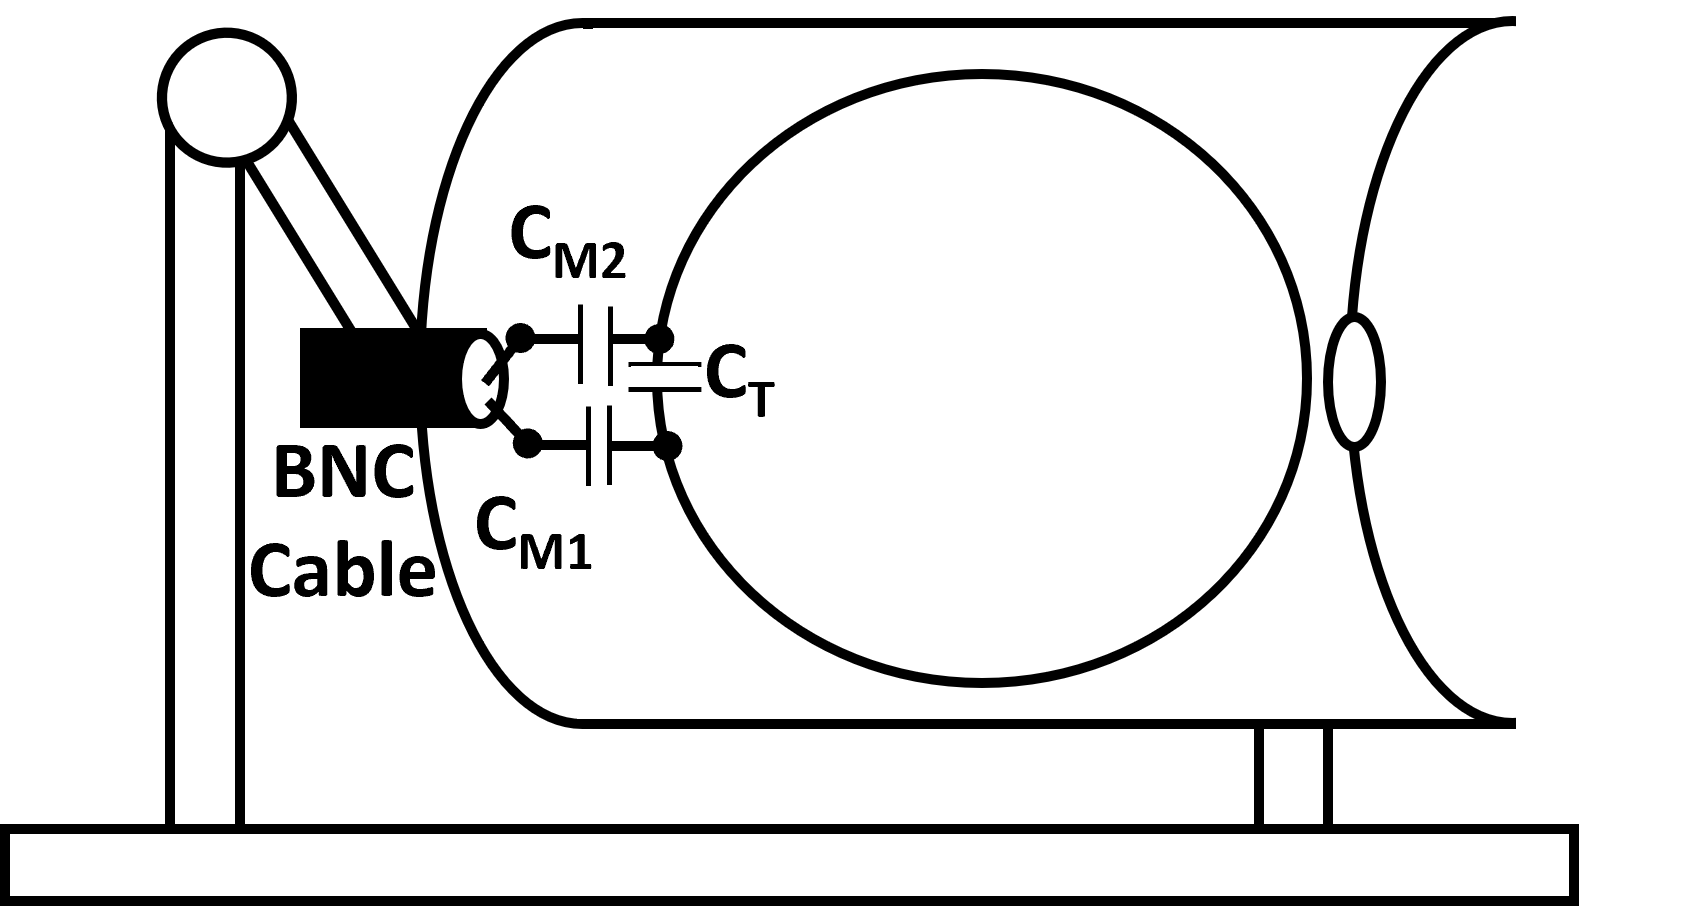
\includegraphics[width=0.7\textwidth]{Figures/Theory/Liver_Coil.png}
    \caption{\textit{Diagram of the circular surface C$_T$ is the tuning capacitor and C$_{M2}$ and C$_{M1}$ are the matching capacitors which are attached to a BNC cable which continues of the diagram. The bottom bar of the diagram is housing which slides into the \ac{MRI} bed, then the two spokes then hold the coil in plastic housing. The circular joint in the top-left of the image allows movement so the coil can be comfortable and close to the participant.}}
    \label{fig:theory:Liver}
\end{figure}

The second coil is 12 cm in diameter and again made out of copper wire, and is designed for imaging the liver. This coil is larger so that the penetration depth is large enough to reach the liver. The coil is slightly curved in plane in order for the coil to sit closer to the liver on one side of the abdomen and is mounted onto a holder so that the coil can be rotated whilst still being attached to the scanner bed.

\begin{figure}
    \centering
    \includegraphics[width=0.9\textwidth]{Figures/Theory/Coil_Pics.png}
    \caption{\textit{Photos of the calf surface coil from two different angles (a \& b) with a photo of the liver surface coil (c), both tuned to the $^2$H Larmor frequency at 3T. The yellow tablets that can be seen in all the photos are vitamin tablets (also known as fiducial markers) used to identify where the coil is in an image.}}
    \label{fig:theory:Pics}
\end{figure}

\subsubsection{Saddle}

\begin{figure}
    \centering
    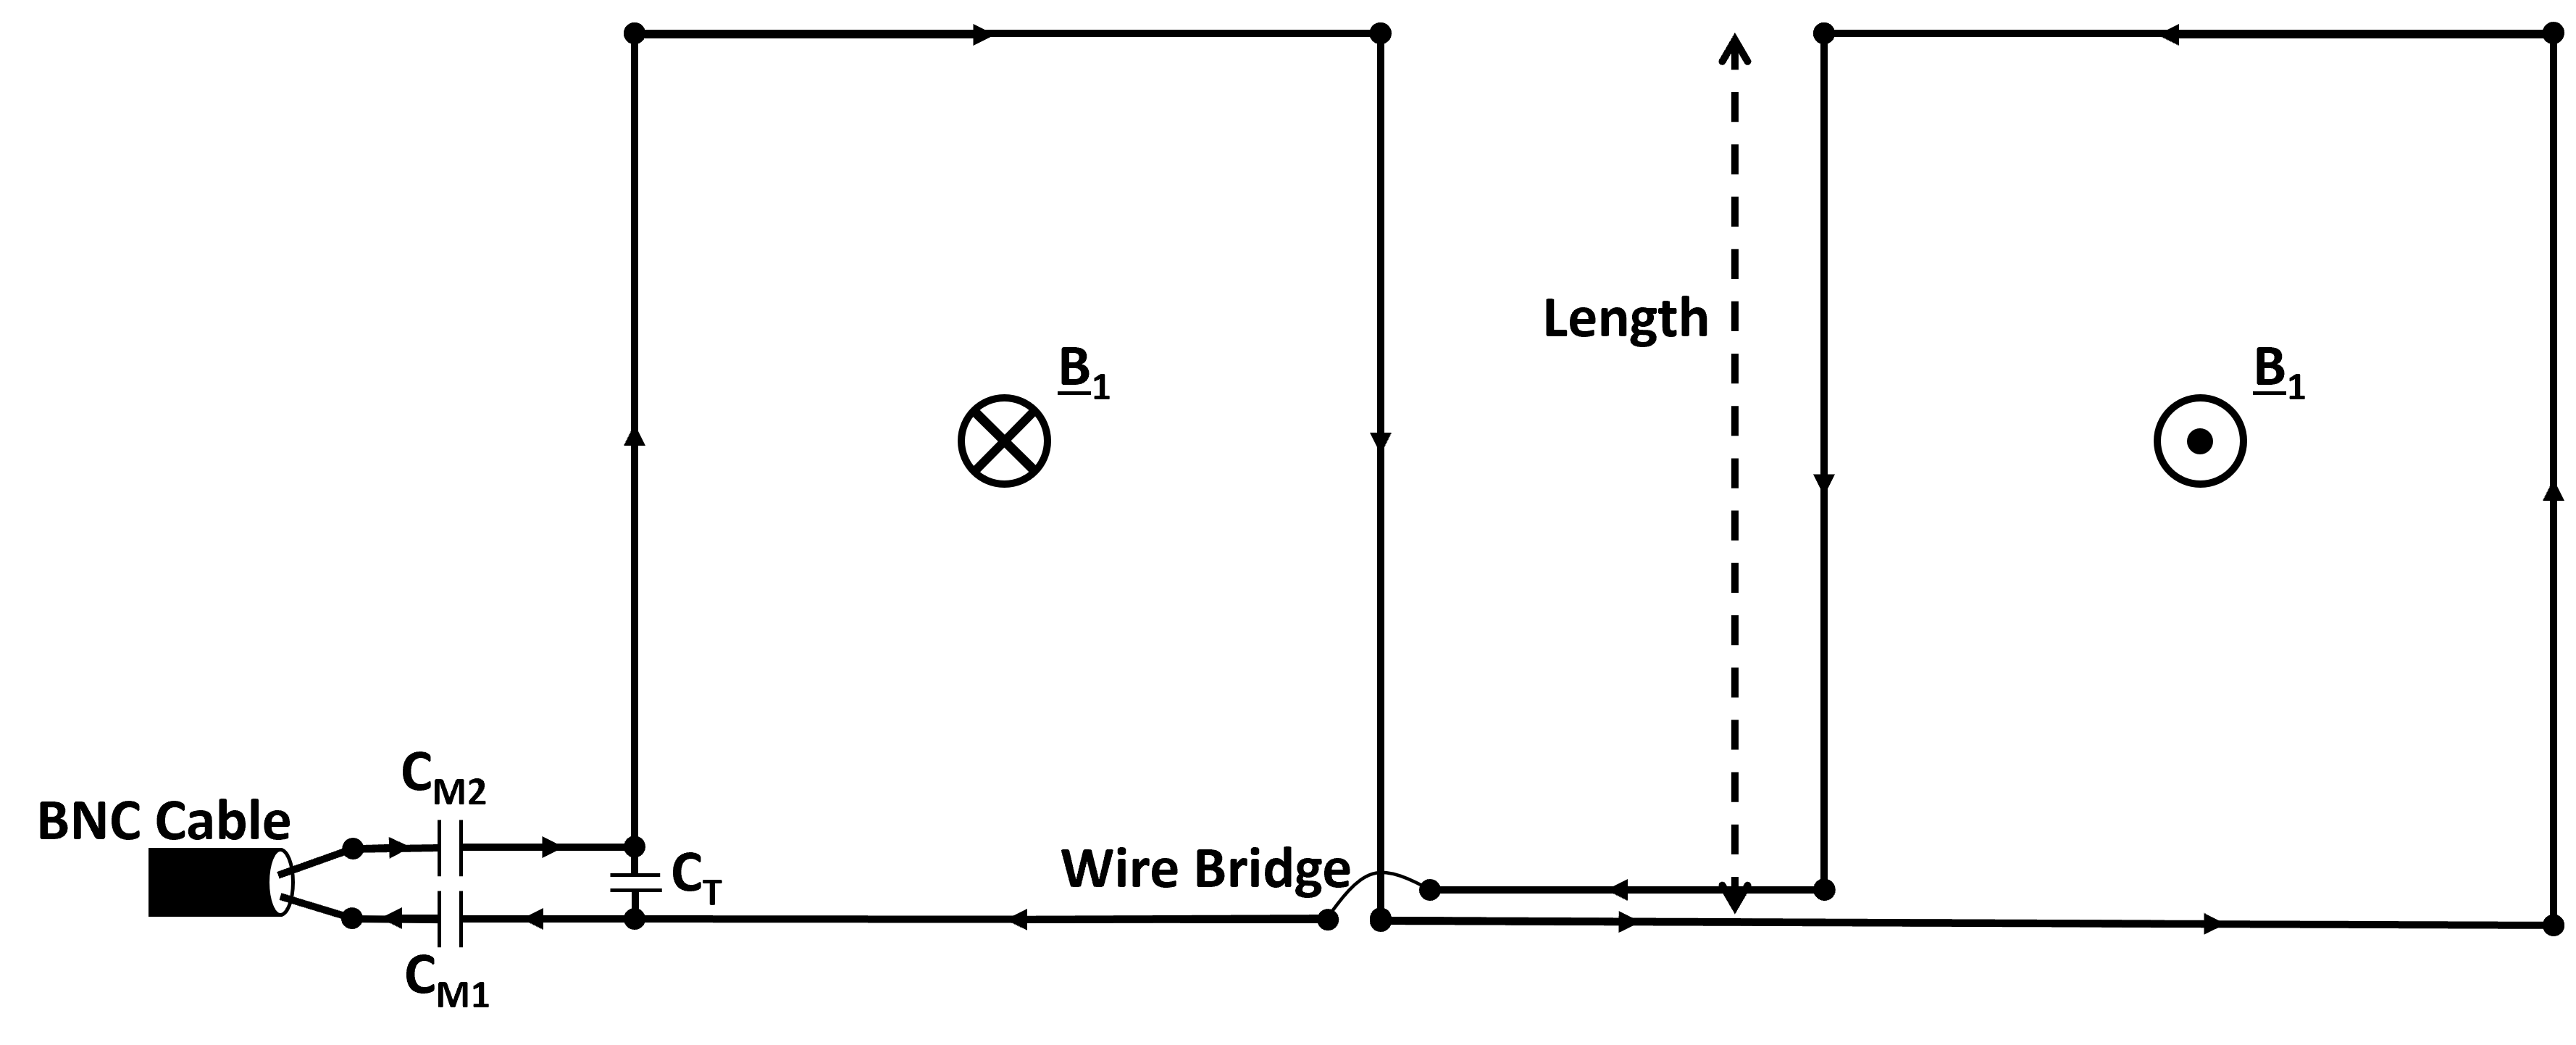
\includegraphics[width=1\textwidth]{Figures/Theory/Planar_Saddle.png}
    \caption{\textit{2D circuit diagram of the saddle coil used for scanning of the calf.}}
    \label{fig:theory:2D_Saddle}
\end{figure}

Volumetric coils such as saddle coils have more homogeneous B$_1$ fields than surface coils and are able to cover a larger volume. A saddle coil derives its name from the fact that the coil elements it uses have a similar appearance to a horse's saddle. Two square loops surround a circular tube with an angular separation of 120$^\circ$ of the wires in each saddle. The saddle coil has optimum geometry that has been previously been found which includes the length/diameter between 1 and 2, and an angular width for each coil of $\approx$120$^\circ$ \cite{Ginsberg1970OptimumField,Salmon2006OptimizationImaging}.

\begin{figure}
    \centering
    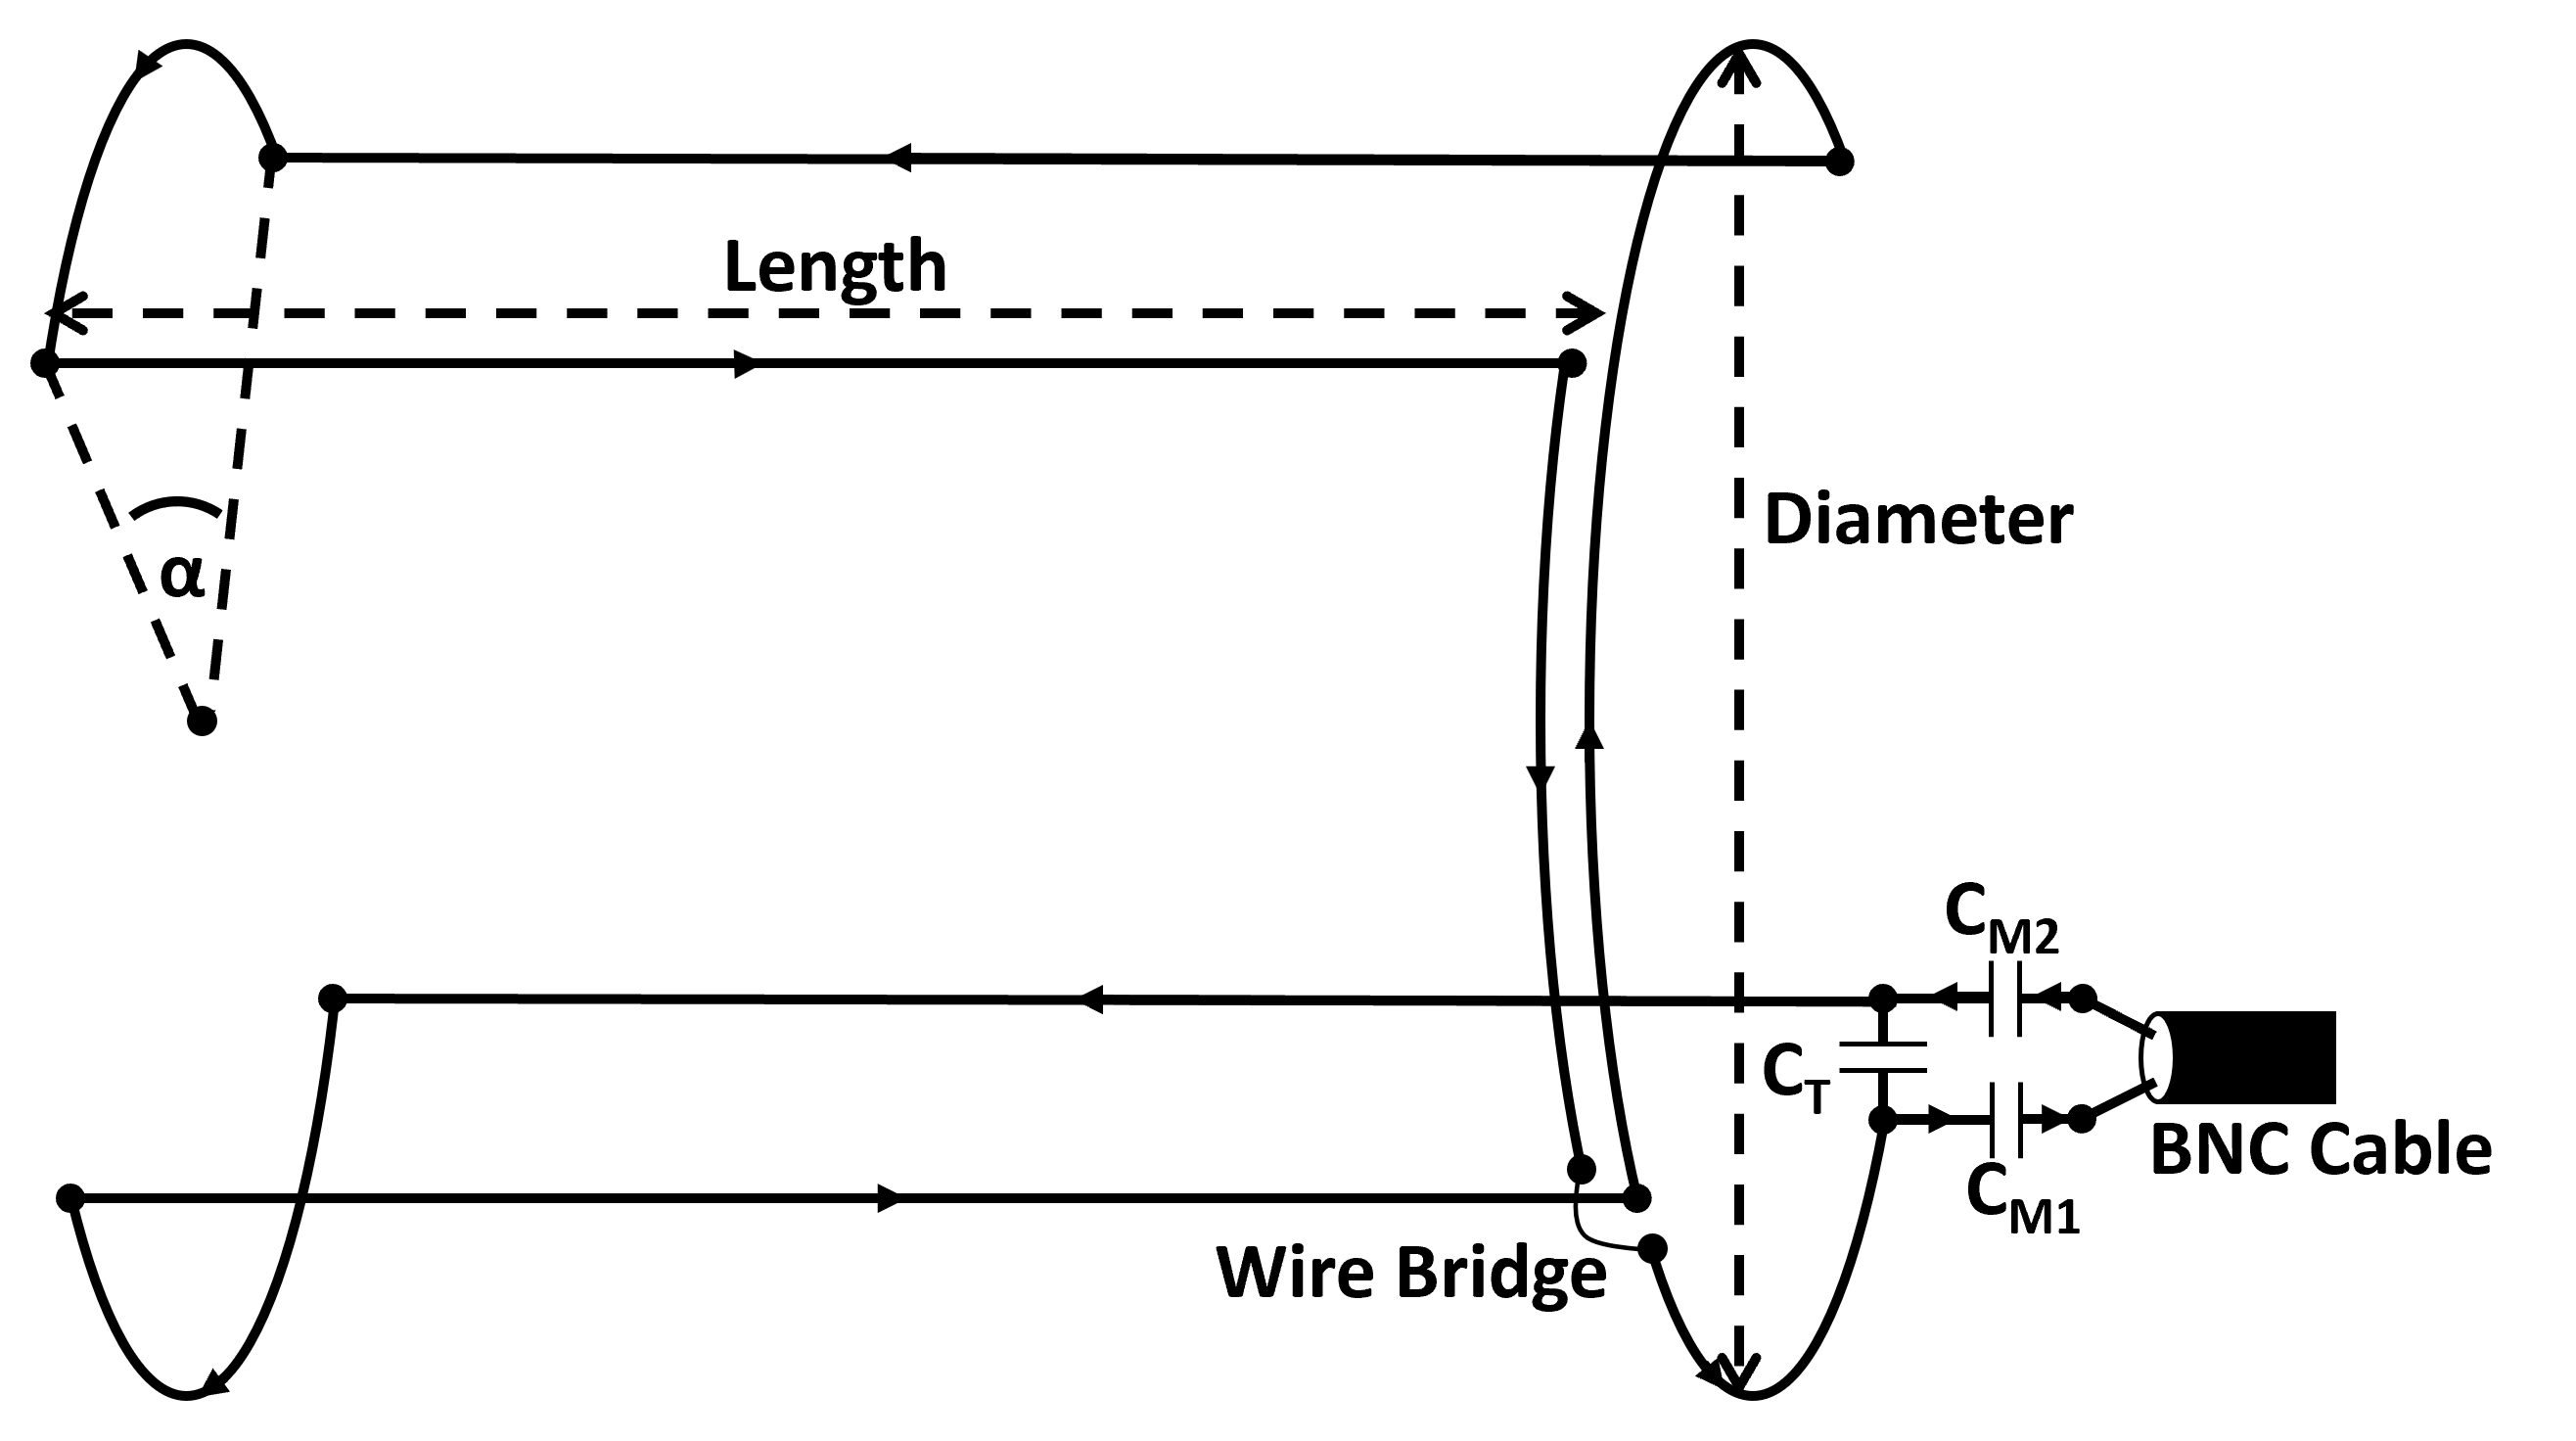
\includegraphics[width=0.8\textwidth]{Figures/Theory/3D_Saddle.png}
    \caption{\textit{3D circuit diagram of the saddle coil used for scanning of the calf.}}
    \label{fig:theory:3D_Saddle}
\end{figure}

The coil built for scanning in Chapter \ref{Chap:Quad} is made from copper tape and has an angular width of 120$^\circ$ a length of 16.8 cm and a diameter of 14.8 cm. Where the copper tape that links the two squares intersects/crosses over, an insulated wire is used to avoid a capacitor being created. Also, the wires here run close side by side so that the fields from the opposing currents will cancel. Diagrams of the circuit for the coil are shown in Figs. \ref{fig:theory:2D_Saddle} and \ref{fig:theory:3D_Saddle} with pictures in Fig. \ref{fig:theory:Saddle_pic}. The tuning capacitance is 47.3 pF, the total matching capcitance 8.8 pF.

\begin{figure}
    \centering
    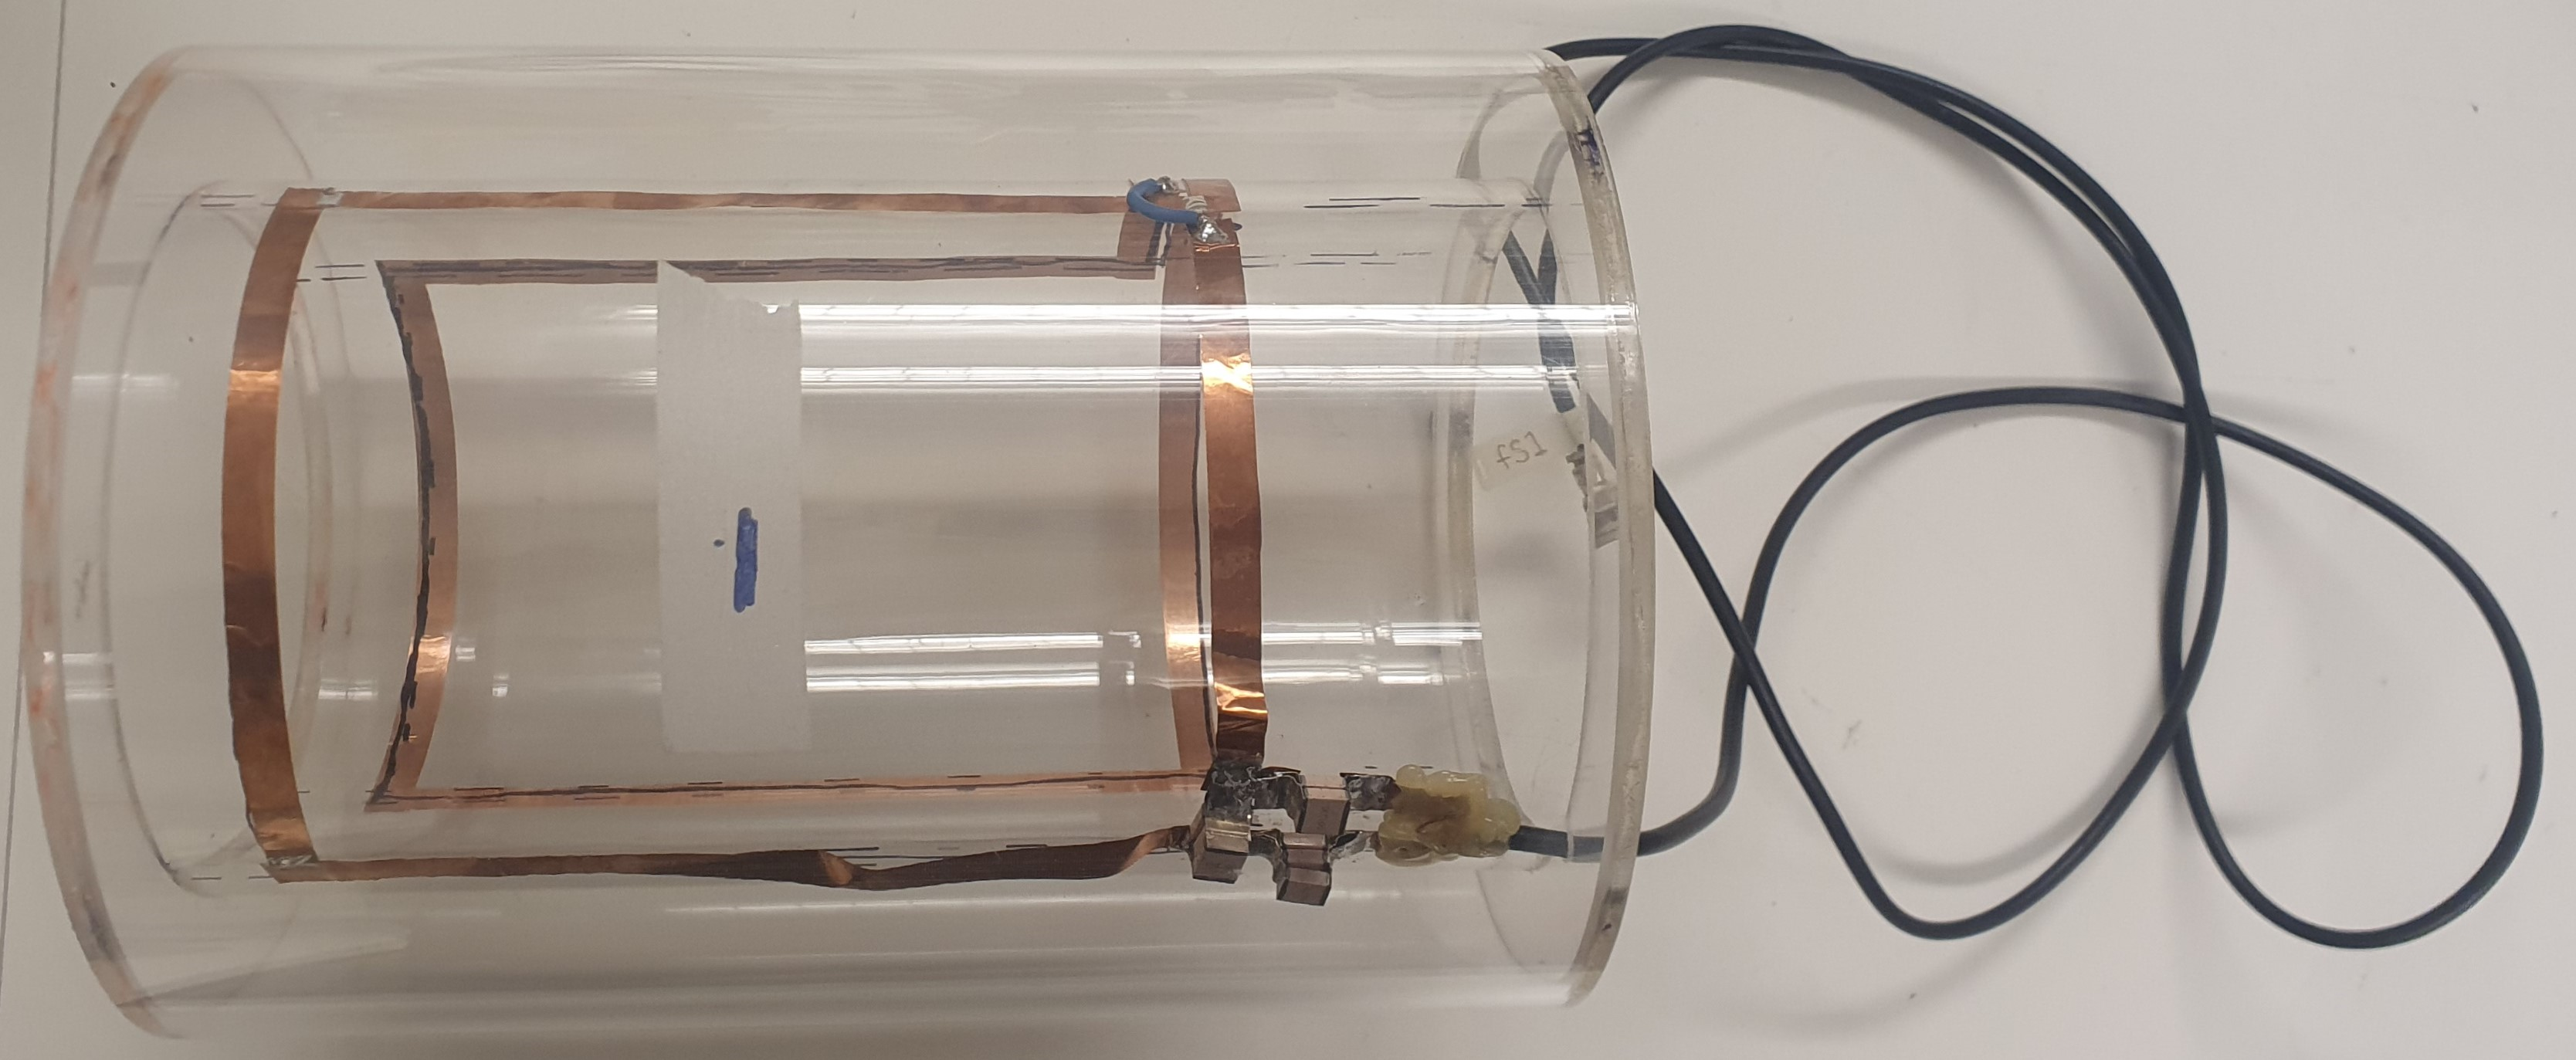
\includegraphics[width=1\textwidth]{Figures/Theory/Saddle_Coil.jpg}
    \caption{\textit{Photo of the saddle coil used to obtain $^2$H data from the calf.}}
    \label{fig:theory:Saddle_pic}
\end{figure}

\subsubsection{Helmholtz coil}

\begin{figure}
    \centering
    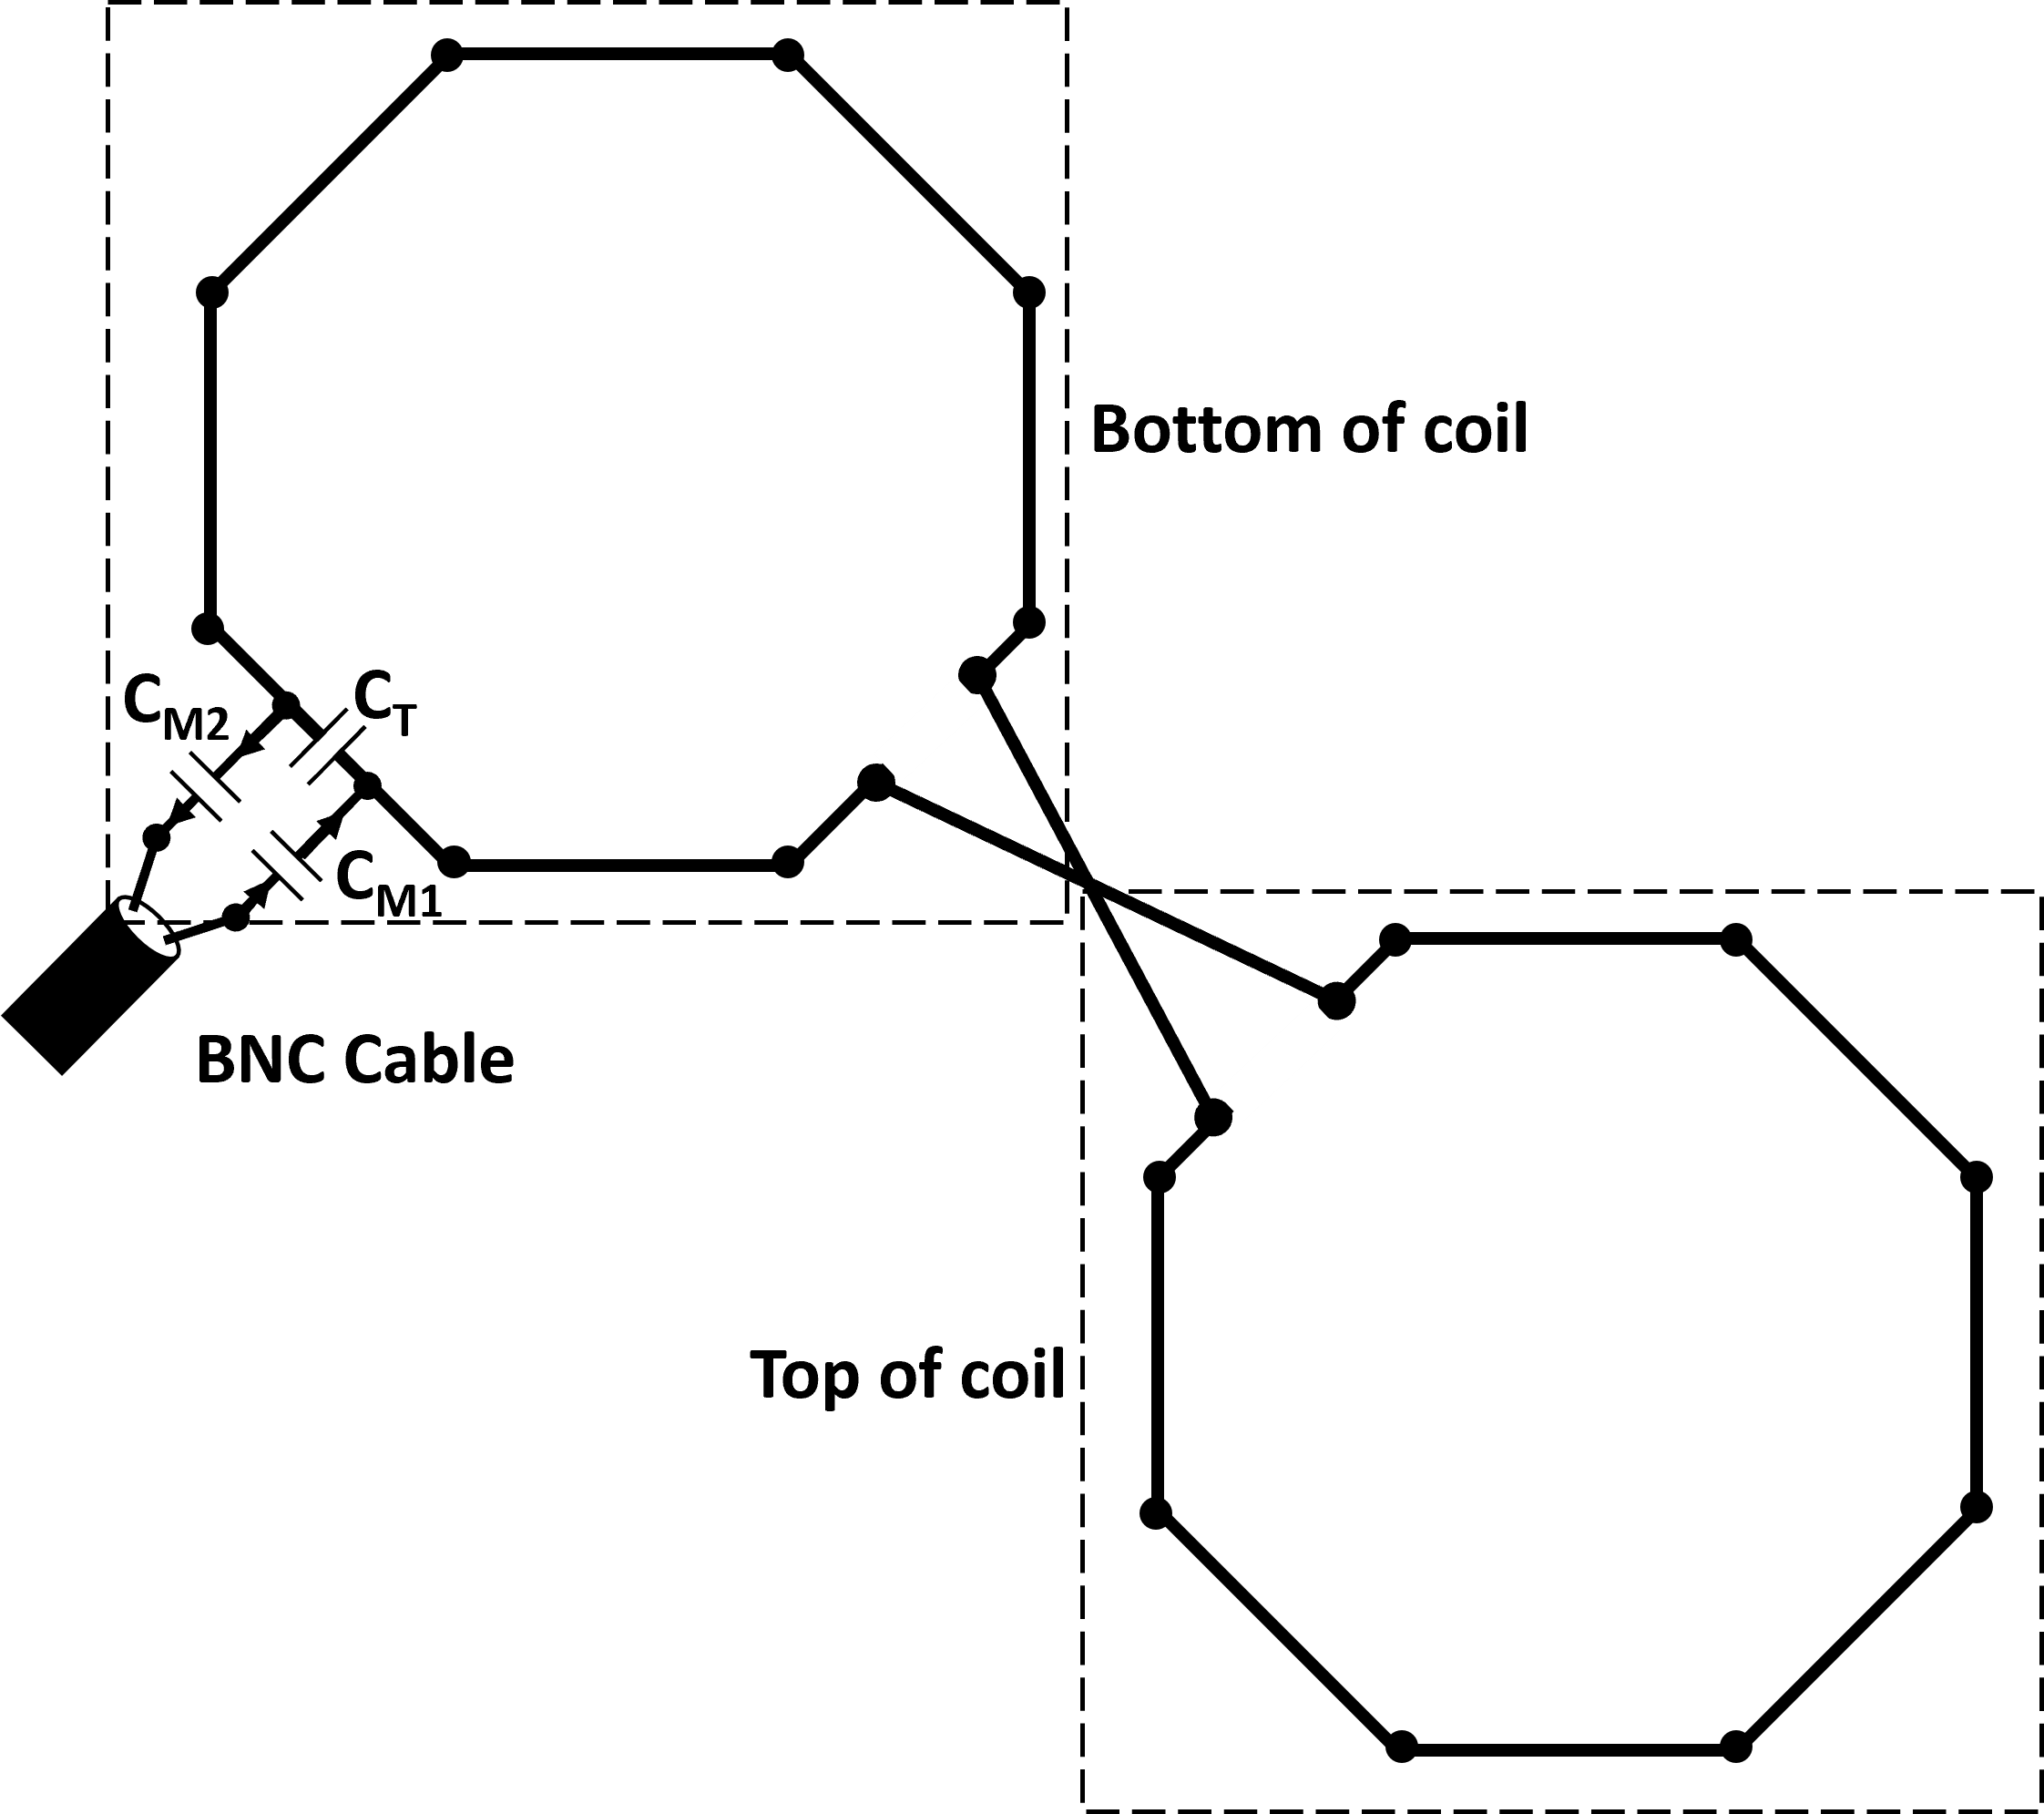
\includegraphics[width=0.8\textwidth]{Figures/Theory/Planar_Helmholtz.png}
    \caption{\textit{2D circuit diagram of the Helmholtz coil used for scanning of the arm.}}
    \label{fig:theory:2D_Helmholtz}
\end{figure}

A Helmholtz coil is similar to to a surface coil in its circuitry. Except a second surface coil is connected to it by two crossing insulated wires, where the current in each flows in opposite directions so that the field flows in the centre of the setup. This creates a homogeneous B$_1$ in between the coils. The Helmholtz coil arrangement was chosen for the scanning the forearm described in Chapter \ref{Chap:Quad} and needs to be easily movable and a saddle coil would roll/move to much and would be difficult to rotate in the magnet bore.

\begin{figure}
    \centering
    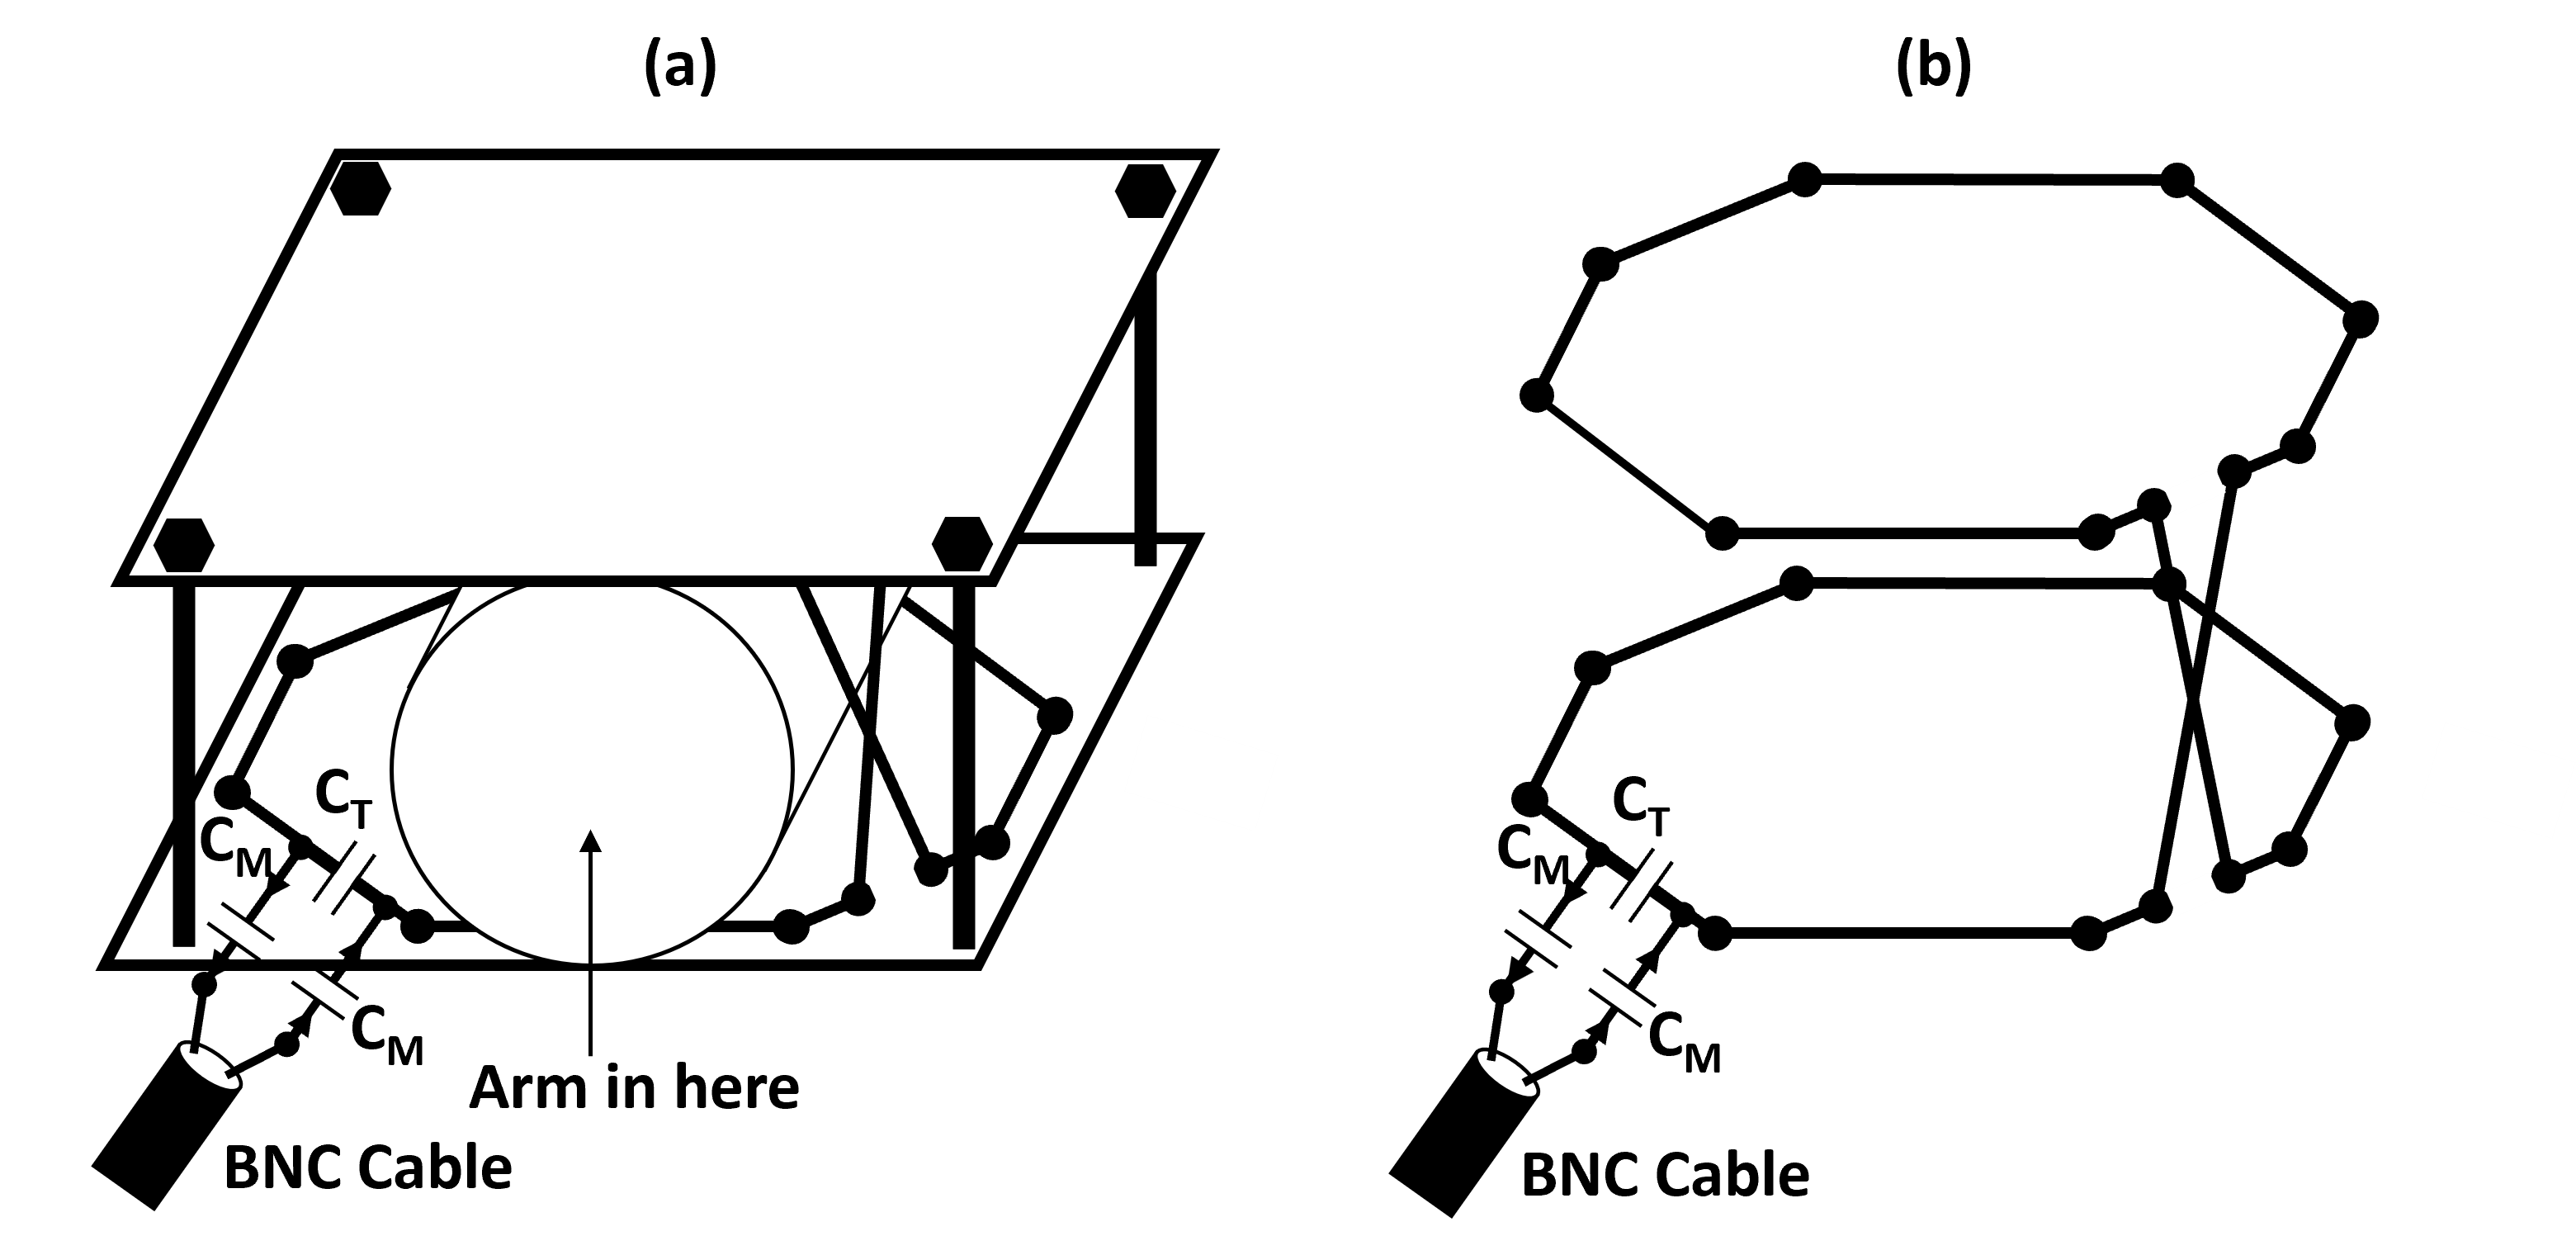
\includegraphics[width=1\textwidth]{Figures/Theory/3D_Helmholtz.png}
    \caption{\textit{3D circuit diagram of the Helmholtz coil used for scanning of the arm with housing (a) and without (b).}}
    \label{fig:theory:3D_Helmholtz}
\end{figure}

The coil setup comprises involves two octagonal loops that are $\approx$14 cm in diameter separated by a 12 cm gap with a tube in the centre to keep the arm still in the same position, away from the circuit elements. The tuning capacitance is 73.3 pF and the total matching capacitance is 8.8 pF.

\begin{figure}
    \centering
    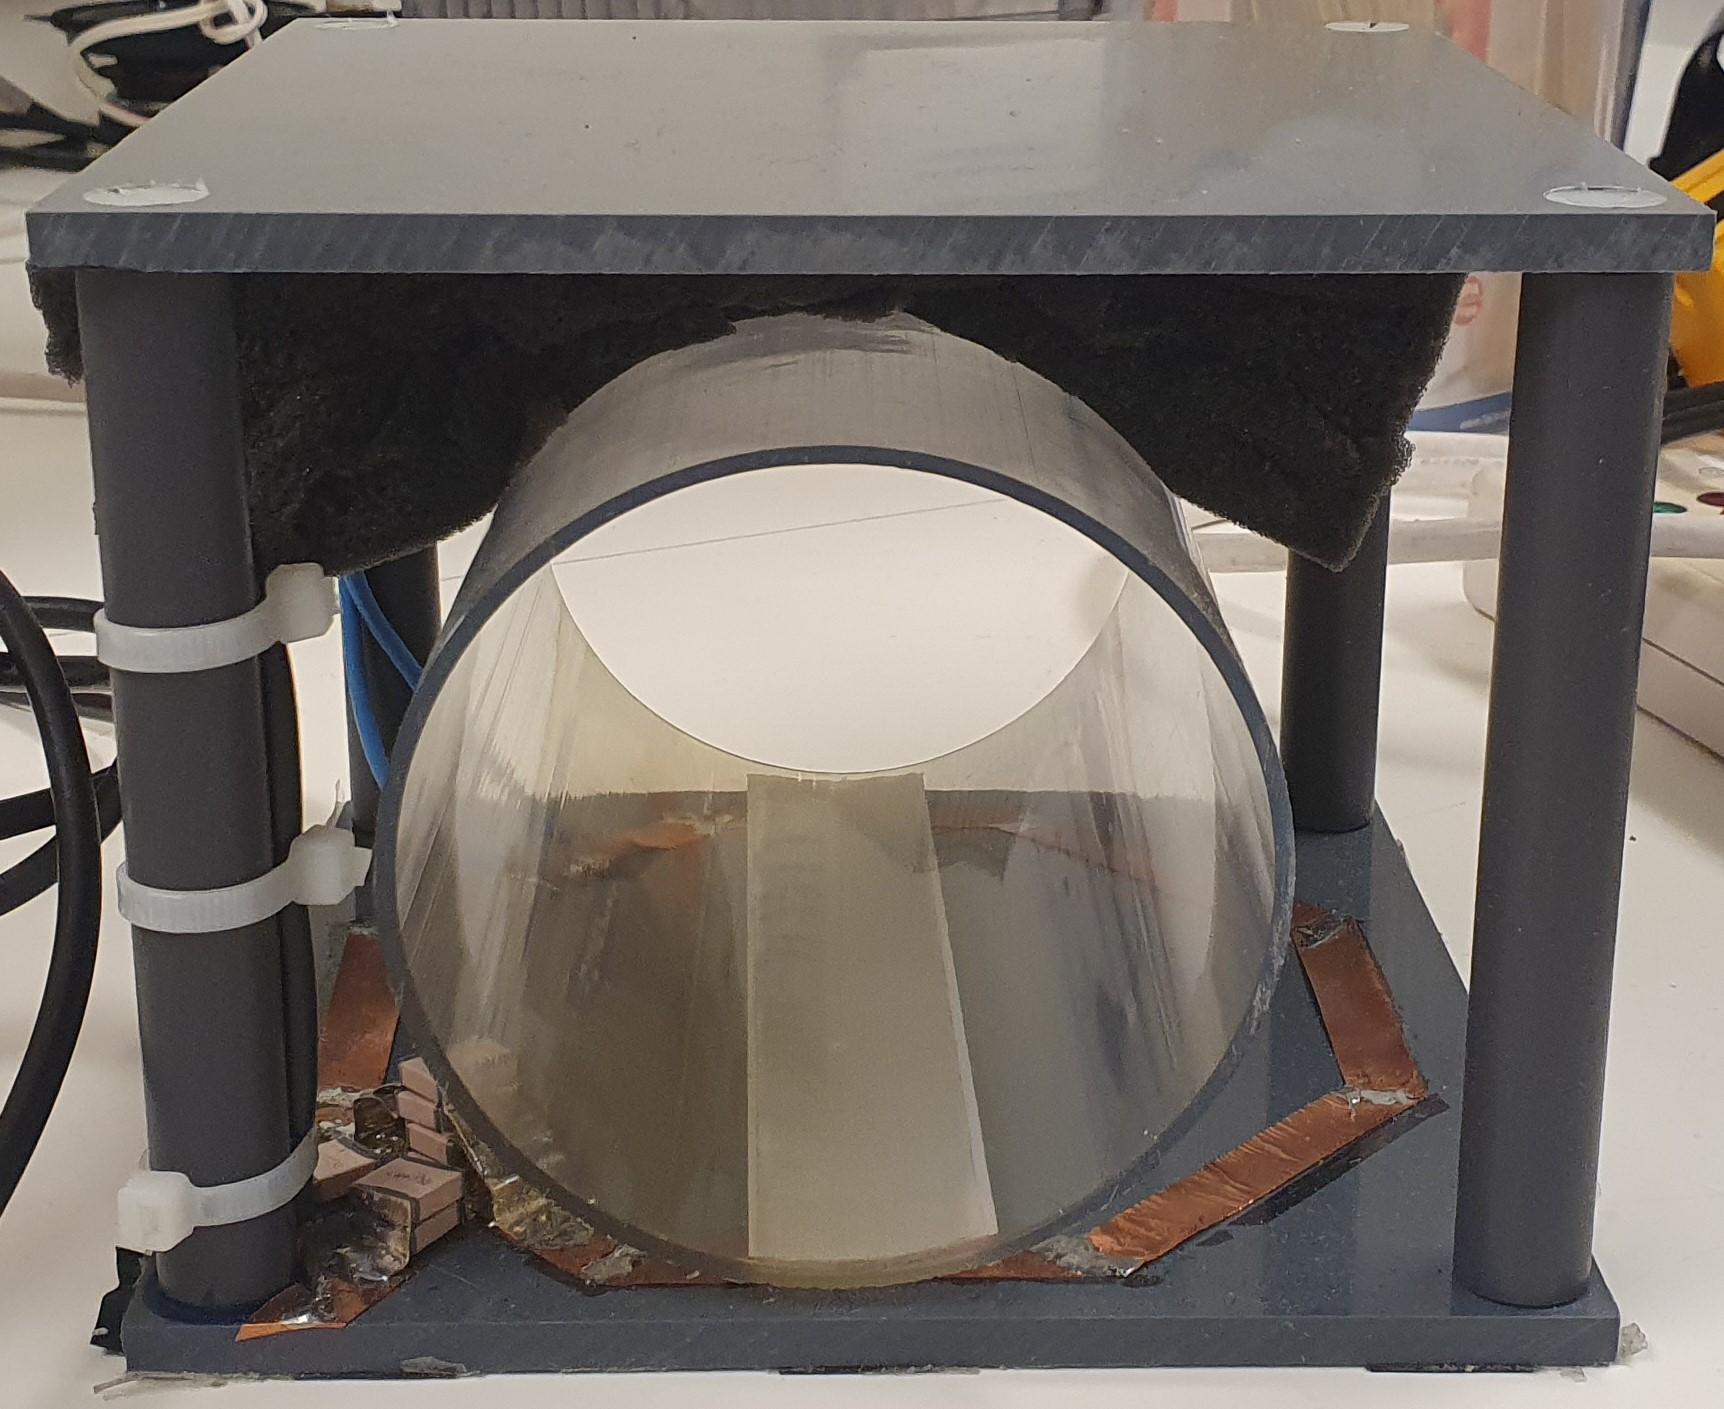
\includegraphics[width=0.8\textwidth]{Figures/Theory/HelmHoltz_Coil.jpg}
    \caption{\textit{Photo of the HelmHoltz coil used to obtain $^2$H data from the arm.}}
    \label{fig:theory:HelmHoltz_pic}
\end{figure}